\documentclass[11pt]{article}

\usepackage[english]{babel}
\usepackage[top=1in,bottom=1.2in,left=1in,right=1in]{geometry}
\usepackage{amssymb,amsmath,amsthm,mathtools}
\usepackage{mathrsfs}
\usepackage{times}
\usepackage{graphicx}
\usepackage{placeins}
\usepackage{hyperref}

\hypersetup{
  colorlinks=true,
  linkcolor=blue,
  citecolor=red,
  urlcolor=blue,
  pdfauthor={}
}

\newtheorem{theorem}{Theorem}[section]
\newtheorem{proposition}[theorem]{Proposition}
\newtheorem{lemma}[theorem]{Lemma}
\newtheorem{corollary}[theorem]{Corollary}
\theoremstyle{definition}
\newtheorem{remark}[theorem]{Remark}

\numberwithin{equation}{section}

\newcommand{\E}{\mathbb{E}}
\newcommand{\Pbb}{\mathbb{P}}
\newcommand{\R}{\mathbb{R}}
\newcommand{\cN}{\mathcal{N}}
\newcommand{\wh}{\widehat}
\newcommand{\eps}{\varepsilon}
\newcommand{\cJ}{\mathcal J}
\newcommand{\cP}{\mathcal P}
\DeclareMathOperator{\Var}{Var}
\DeclareMathOperator{\supp}{supp}

\title{Variance Misspecification and the One-Dimensional Gaussian Mixture NPMLE}
\author{}
\date{}

\begin{document}

\maketitle

\begin{abstract}
Can a one-atom Gaussian mixture NPMLE serve as evidence that a sample comes
from a single population? Without regularization the answer is no: even under
one Gaussian component, the fitted support diverges. We study whether a small
variance inflation prevents this spurious support growth. The observations are i.i.d.\
\(\cN(0,1-\eps_n)\), while the fitted location mixture uses unit-variance
Gaussian components.

If \(\eps_n=n^{-r_n}\) and \(r_n\to r\), the one-atom probability converges to
a phase curve \(p(r)\). The curve is continuous, equals one at \(r=0\), is
strictly decreasing on \((0,1/4)\), and vanishes for \(r\ge1/4\). We identify
its behavior at both endpoints; the upper endpoint is governed by the
persistence exponent of a stationary Gaussian process. The limiting curve is
defined through two independent compensated Poisson edge fields, which arise
from the upper and lower sample extremes. More generally, for \(r<1/4\) the
entire fitted atom count converges to an integer-valued law that depends only
on \(r\) and varies continuously with \(r\). These limiting counts diverge in probability
as \(r\uparrow1/4\), whereas the finite-sample counts are uniformly tight
whenever \(\limsup r_n<1/4\).
\end{abstract}

\medskip
\noindent\textbf{Note.} This draft was produced through an iterative process in which Mark Sellke repeatedly asked GPT-5.6 in OpenAI Codex to prove, refine, and write up further extensions.
\medskip

\setcounter{tocdepth}{1}
\tableofcontents

\section{Introduction}

Can one detect from a finite sample whether the data come from a single
Gaussian by fitting a Gaussian mixture model? For the nonparametric maximum
likelihood estimator, this becomes a question about the fitted mixing
distribution: does maximum likelihood choose one component mean, or does it
introduce additional atoms? Polyanskiy and Wu asked how many atoms the NPMLE
selects even under one Gaussian component
\cite[Section~5.6]{polyanskiy2020self}. Our companion paper shows that, when
the fitted component variance matches the data-generating variance, the
support in fact diverges in probability \cite{supportDivergenceCompanion}.
Thus an unregularized atom count is not by itself a calibrated diagnostic of
latent heterogeneity.

Here we ask whether fitting slightly wider Gaussian components prevents this
spurious growth of the fitted support.
Let \(Z_1,\dots,Z_n\) be i.i.d.\ \(\cN(0,1)\), and observe
\begin{equation}
\label{eq:model-intro}
    X_i=\sqrt{1-\eps_n}\,Z_i,
    \qquad 0\le\eps_n<1.
\end{equation}
We fit location mixtures of unit-variance Gaussians. Thus the fitted kernels
are slightly wider than the data-generating component, and spreading the
mixing distribution incurs a deterministic variance penalty. Our main results
determine the scale at which this penalty first makes a one-atom fit optimal.

For a probability measure \(G\) on \(\R\), write
\[
    q_G(x)=\int_\R\phi(x-u)\,dG(u),
    \qquad
    \ell_n(G)=\sum_{i=1}^n\log q_G(X_i),
\]
where \(\phi\) and \(\Phi\) are the standard normal density and distribution
function, respectively. Let \(\wh G_n\) maximize
\(\ell_n\) over all probability measures on \(\R\). The one-dimensional
Gaussian-mixture NPMLE is almost surely unique
\cite{lindsay1993uniqueness}, so its support size is unambiguous.

The geometry behind the transition is simple to state. Put
\(Y_i=X_i-\bar X_n\) and
\begin{equation}
\label{eq:D-intro}
    D_n(a)=\frac1n\sum_{i=1}^n
       \exp\left(aY_i-\frac{a^2}{2}\right).
\end{equation}
The measure \(\delta_{\bar X_n}\) is an NPMLE if and only if
\(\sup_aD_n(a)\le1\). For the sample with variance defect \(\eps\), denote
this field by \(D_{n,\eps}\). After writing \(t=a\sqrt{1-\eps}\),
\[
    D_{n,\eps}(a)=e^{-\kappa(\eps)t^2}K_n(t),
    \qquad
    \kappa(\eps)=\frac{\eps}{2(1-\eps)},
\]
where \(K_n\) depends only on the standardized sample \(Z_{1:n}\). Increasing
\(\eps\) therefore suppresses every nonzero perturbation and can only favor a
one-atom fit. Lemma~\ref{lem:variance-monotonicity} proves that the one-atom
set is an upper interval in \(\eps\). We may therefore define the samplewise
critical inflation
\[
    \eps_{*,n}
    =\inf\left\{\eps\in[0,1):
       \sqrt{1-\eps}\,Z_1,\dots,\sqrt{1-\eps}\,Z_n
       \text{ have a one-atom NPMLE}\right\},
\]
and its exponent
\[
    R_{*,n}=-\frac{\log\eps_{*,n}}{\log n},
    \qquad -\log0:=\infty.
\]

This monotonicity is the deterministic foundation of the paper, and it is
specific to one atom. Proposition~\ref{prop:full-support-nonmonotonicity}
shows how completely monotonicity fails for larger support counts: for any
\(m\ge2\) and any component variances \(S<T\),
a finite sample can have \(m\) atoms at variance \(T\) and two at variance
\(S\). The value two is optimal, since a path that is one-atomic at \(S\)
remains one-atomic at every larger variance. Thus one-atomicity has a
well-defined critical variance, whereas no larger support threshold is
monotone.

The nontrivial scale is polynomial. Choose \(u_n\) so that
\(n\Pbb\{Z>u_n\}=1\). The rescaled upper-edge points
\(u_n(Z_i-u_n)\) converge to a Poisson point process on \(\R\) with intensity
\(e^{-x}\,dx\). For score locations \(t=\theta u_n\),
\(1/2<\theta<1\), the centered directional field converges to a compensated
Poisson integral. The lower sample edge gives an independent copy.

Let \(N\) be a Poisson point process on \(\R\) with intensity
\(\mu(dx)=e^{-x}\,dx\). For \(1/2<\theta<1\), define
\begin{equation}
\label{eq:S-intro}
    S(\theta)=\int_\R e^{\theta x}\{N-\mu\}(dx).
\end{equation}
The integral on \((-\infty,0)\) is a compensated \(L^2\) limit. On
\([0,\infty)\), the process has only finitely many points almost surely, so
the integral is the ordinary Poisson sum minus its compensator. This split is
important: the positive-tail contribution need not be square-integrable.

Let \(S_+\) and \(S_-\) be independent copies of \(S\). For
\(0<r<1/4\), set \(\theta_r=1-\sqrt r\) and
\begin{equation}
\label{eq:p-intro}
    p(r)=
    \Pbb\left\{
       \max_{\xi\in\{+,-\}}
       \sup_{\theta_r\le\theta<1}S_\xi(\theta)\le0
    \right\}.
\end{equation}
Extend \(p\) to \([0,\infty]\) by \(p(0)=1\) and
\(p(r)=0\) for \(r\ge1/4\).

The first theorem identifies the limiting one-atom probability at every
polynomial exponent and, equivalently, the law of the samplewise critical
inflation.
\begin{theorem}
\label{thm:exponent-phase-diagram}
Assume \(0<\eps_n<1\), and write \(\eps_n=n^{-r_n}\). If
\(r_n\to r\in[0,\infty]\), then
\[
    \Pbb\{|\supp(\wh G_n)|=1\}\longrightarrow p(r).
\]
More generally, if \(\liminf_{n\to\infty}r_n\ge1/4\), then
\(\Pbb\{|\supp(\wh G_n)|=1\}\to0\).
\end{theorem}

Together with the continuity in Proposition~\ref{prop:phase-curve-properties},
this is equivalent to \(R_{*,n}\Rightarrow R_*\), where
\[
    \Pbb\{R_*\ge r\}=p(r),
    \qquad 0<r<1/4.
\]

The limiting curve has no flat pieces in its nontrivial interval. Its two
endpoints are governed by different mechanisms: one large Poisson point near
\(r=0\), and Gaussian persistence near \(r=1/4\).
\begin{proposition}
\label{prop:phase-curve-properties}
The function \(p\) is continuous and nonincreasing on \([0,\infty]\), strictly
decreasing on \((0,1/4)\), and satisfies \(0<p(r)<1\) there. Moreover,
\[
    1-p(r)\sim2\sqrt r
    \qquad(r\downarrow0),
\]
while
\[
    p(r)=\left(\frac14-r\right)^{3/8+o(1)}
    \qquad(r\uparrow1/4).
\]
\end{proposition}

Near the upper endpoint, the small jumps of the Poisson field are coupled to
a stationary Gaussian process with sech covariance. Its one-sided persistence
exponent is \(3/16\)
\cite{DemboPoonenShaoZeitouni2002,FitzGeraldTribeZaboronski2022}; the two
independent sample edges double this to \(3/8\). The transfer from the Poisson
field uses a Koml\'os--Major--Tusn\'ady (KMT) strong approximation and the
small-level persistence estimates
of Feldheim--Feldheim--Mukherjee
\cite{komlos1975approximation,komlos1976approximation,FeldheimFeldheimMukherjee2025}.

Figure~\ref{fig:phase-curve} illustrates the phase curve and the two endpoint
asymptotics.
\begin{figure}[ht]
    \centering
    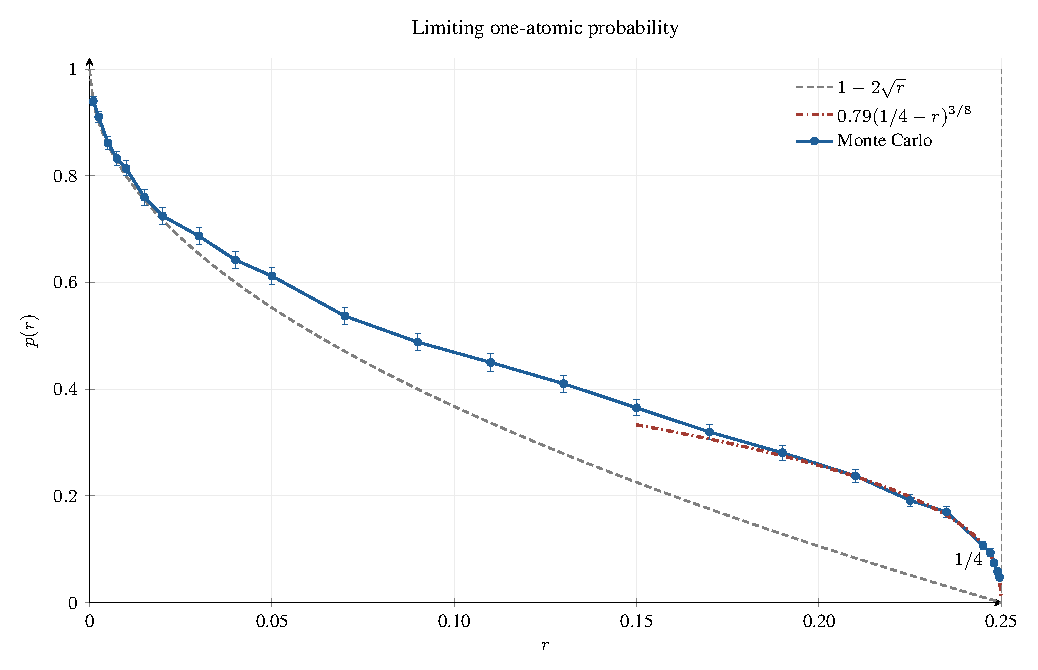
\includegraphics[width=0.82\textwidth]{figures/phase_curve.pdf}
    \caption{Numerical illustration of the limiting one-atom phase curve. The
    blue points are Monte Carlo estimates of \(p(r)\), with
    two-standard-error bars, and the gray dashed line is the lower-endpoint
    asymptotic \(1-2\sqrt r\). Proposition~\ref{prop:phase-curve-properties}
    proves that \(p(r)=(1/4-r)^{3/8+o(1)}\) as \(r\uparrow1/4\); numerically,
    \(0.79(1/4-r)^{3/8}\) appears to match near the endpoint, as shown by the
    red dot-dashed line.}
    \label{fig:phase-curve}
\end{figure}
\FloatBarrier

The Poisson limit also determines the entire support size. For
\(b\in(1/2,1)\), a finite positive measure \(\nu\) compactly supported in
\([b,1)\), and \(h(y)=\log(1+y)-y\), put
\begin{equation}
\label{eq:atom-limit-functional}
    F_\nu(x)=\int e^{\theta x}\,\nu(d\theta),
    \qquad
    \cJ_{N,b}(\nu)
    =\int S(\theta)\,\nu(d\theta)
      +\int_{\mathbb R}h\{F_\nu(x)\}\,N(dx).
\end{equation}
Proposition~\ref{prop:atom-limit-unique} proves that \(\cJ_{N,b}\) has an
almost surely unique optimizer \(\nu_b^*\). Let
\(\nu_b^{*,+}\) and \(\nu_b^{*,-}\) be the optimizers constructed from two
independent copies of \(N\). Define \(\mathsf K_0=1\) and, for
\(0<r<1/4\),
\begin{equation}
\label{eq:atom-count-intro}
    \mathsf K_r
    =1+|\supp(\nu_{1-\sqrt r}^{*,+})|
       +|\supp(\nu_{1-\sqrt r}^{*,-})|.
\end{equation}
The next theorem shows that this explicit Poisson functional gives the unique
limit of the fitted support size.
\begin{theorem}
\label{thm:atom-count-limit}
If \(\eps_n=n^{-r_n}\) and \(r_n\to r<1/4\), then
\[
    |\supp(\wh G_n)|\Rightarrow\mathsf K_r.
\]
For \(0<r<1/4\),
\[
    \Pbb\{\mathsf K_r=1\}=p(r).
\]
The map \(r\mapsto\mathcal L(\mathsf K_r)\) is continuous in total variation
on \([0,1/4)\).
\end{theorem}

Although each interior limiting law is finite, the Poisson optimizer becomes
increasingly complex as its hard wall approaches \(1/2\). The endpoint
likelihood comparison gives a lower bound for its atom count at the scale
\(\log(1/\delta)/\log\log(1/\delta)\).
\begin{proposition}
\label{prop:atom-count-endpoint-divergence}
For \(0<\delta<1/4\), set \(r_\delta=1/4-\delta\). Then
\[
    \lim_{\eta\downarrow0}\limsup_{\delta\downarrow0}
    \Pbb\left\{
       \mathsf K_{r_\delta}
       \le \eta\frac{\log(1/\delta)}{\log\log(1/\delta)}
    \right\}=0.
\]
In particular, \(\mathsf K_r\to\infty\) in probability as
\(r\uparrow1/4\).
\end{proposition}

Proposition~\ref{prop:atom-count-endpoint-divergence} concerns the limiting
variables \(\mathsf K_r\): one first takes the sample-size limit with \(r\)
fixed and then lets \(r\uparrow1/4\). It does not give a uniform
finite-sample approximation for a triangular sequence \(r_n\uparrow1/4\).

The convergence theorem also gives uniform tightness away from the critical
endpoint: if \(\limsup_n r_n<1/4\), then
\(|\supp(\wh G_n)|=O_{\mathbb P}(1)\). Indeed, failure along some sequence
would persist along a subsequence on which \(r_n\) converges to a point of
\([0,1/4)\), contradicting Theorem~\ref{thm:atom-count-limit}.

The one-dimensional mechanism is exceptional. In dimensions at least two,
the angular geometry produces logarithmic radial transitions instead of the
two-sided polynomial persistence curve above; that problem, including growing
dimension, is treated in a companion paper
\cite{varianceMultivariateCompanion}.

\subsection{Preliminaries}

We first settle the deterministic geometry of the variance path. The
directional-derivative criterion reduces one-atom optimality to a scalar
supremum, and increasing the variance defect can only lower this supremum.
This makes the samplewise critical inflation well defined. We then show that
no analogous monotonicity survives for any larger support threshold. The
one-atom monotonicity and the counterexamples for larger support thresholds
form the deterministic foundation for the scaling limits proved later.

\subsubsection{Notation and convergence}

All asymptotic notation is as \(n\to\infty\), unless another limit is
specified. For a deterministic positive sequence \(a_n\), the relation
\(X_n=O_{\mathbb P}(a_n)\) means that \(|X_n|/a_n\) is tight, while
\(X_n=o_{\mathbb P}(a_n)\) means that \(X_n/a_n\to0\) in probability.
Deterministic \(O(\cdot)\) and \(o(\cdot)\) have their usual meanings. We
write \(a_n\sim b_n\) if \(a_n/b_n\to1\), \(a_n\ll b_n\) if
\(a_n/b_n\to0\), and \(a_n\lesssim b_n\) if \(a_n\le Cb_n\) for a constant
independent of \(n\). The reverse relations are \(\gg\) and \(\gtrsim\), and
\(a_n\asymp b_n\) means that both one-sided bounds hold. Constants
\(c,C,c_0,C_0,\dots\) may change from line to line.

We write \(X_n\Rightarrow X\) for weak convergence. Random functions on a
compact set \(K\) are viewed in \(C(K)\) with the supremum norm. Point
processes carry the vague topology. For a measure \(G\), \(\supp(G)\) is its
support and \(\delta_x\) is the unit point mass at \(x\). Finally,
\(J\Subset I\) means that the interval \(J\) is compactly contained in
\(I\).
For a measurable function \(f\), we use the empirical-measure notation
\(P_nf=n^{-1}\sum_{i=1}^nf(Z_i)\) and \(Pf=\E f(Z)\), where
\(Z\sim\cN(0,1)\).

We use bracketing only in the support-tightness argument. If \(\mathcal F\)
is a class of measurable functions and \(P\) is a probability measure, an
\(L^1(P)\)-bracket of width \(\eta\) is a pair \([l,u]\) with \(l\le u\),
\(\|u-l\|_{L^1(P)}\le\eta\), and all functions between \(l\) and \(u\).
The bracketing number \(N_{[]}\{\eta,\mathcal F,L^1(P)\}\) is the least
number of such brackets needed to cover \(\mathcal F\).

\subsubsection{One-atom optimality and uniqueness}

The following criterion turns the infinite-dimensional likelihood problem
into a scalar supremum. Its monotonicity outside the sample range will later
exclude score locations beyond the extreme observations.
\begin{lemma}
\label{lem:one-atom-D}
For arbitrary observations \(X_1,\dots,X_n\in\R\), the measure
\(\delta_{\bar X_n}\) is an NPMLE if and only if
\[
    \sup_{a\in\R}D_n(a)\le1,
\]
where \(D_n\) is defined in \eqref{eq:D-intro}. Moreover, \(D_n(0)=1\),
\(D_n\) is strictly decreasing on \((\max_iY_i,\infty)\), and it is strictly
increasing on \((-\infty,\min_iY_i)\).
\end{lemma}

\begin{proof}
For \(a\in\R\) and \(0\le t\le1\), perturb the one-atom measure in the
direction of a second atom:

\[
    G_t=(1-t)\delta_{\bar X_n}+t\delta_{\bar X_n+a}.
\]
Since

\[
 \frac{q_{G_t}(X_i)}{q_{\delta_{\bar X_n}}(X_i)}
 =1-t+t\exp\left(aY_i-\frac{a^2}{2}\right),
\]
the right derivative at \(t=0\) is

\[
 \left.\frac{d}{dt}\ell_n(G_t)\right|_{t=0+}
 =n\{D_n(a)-1\}.
\]
Among point masses, \(\delta_{\bar X_n}\) uniquely maximizes the likelihood.
Concavity of \(G\mapsto\ell_n(G)\), together with Lindsay's
directional-derivative criterion \cite{lindsay1983geometryA}, therefore shows
that it is globally optimal exactly when \(D_n(a)\le1\) for every \(a\).

The identity \(D_n(0)=1\) is immediate. Differentiating gives

\[
    D_n'(a)=\frac1n\sum_{i=1}^n
      (Y_i-a)\exp\left(aY_i-\frac{a^2}{2}\right).
\]
Every summand is negative when \(a>\max_iY_i\), and every summand is positive
when \(a<\min_iY_i\), proving the final assertions.
\end{proof}

The NPMLE is known to be unique in one dimension. For the one-atom event we
will use the following narrower consequence.
\begin{proposition}
\label{prop:one-atom-unique}
Let \(n\ge2\) and let \(X_1,\dots,X_n\) be i.i.d.\ from a nondegenerate
Gaussian distribution. Almost surely, if a one-atom NPMLE exists, then it is
the unique NPMLE.
\end{proposition}

\begin{proof}
The only possible one-atom maximizer is \(G_0=\delta_{\bar X_n}\). Suppose
that \(G_0\) and a different mixing measure \(G\) both maximize the
likelihood. Strict concavity of
\((q_1,\dots,q_n)\mapsto\sum_i\log q_i\) implies

\[
    q_G(X_i)=q_{G_0}(X_i),\qquad 1\le i\le n;
\]
otherwise their midpoint would have larger likelihood. Lemma
\ref{lem:one-atom-D} gives \(D_n(a)\le1\) for every \(a\), while

\[
    \int D_n(u-\bar X_n)\,dG(u)
    =\frac1n\sum_{i=1}^n\frac{q_G(X_i)}{q_{G_0}(X_i)}=1.
\]
Thus \(D_n(u-\bar X_n)=1\) for \(G\)-almost every \(u\). Since
\(G\ne G_0\), there is a nonzero \(a\) with \(D_n(a)=1\).

It remains to show that such a contact has probability zero on the one-atom
event. Regard the centered sample \(Y=(Y_1,\dots,Y_n)\) as a Gaussian vector
in the hyperplane \(\mathcal H=\{y\in\R^n:\sum_i y_i=0\}\). Its law is
spherical and nondegenerate on \(\mathcal H\), so \(Y=RU\), where \(R>0\)
is independent of \(U\) and has a density. For a centered sample \(rU\), set

\[
    \mathcal D_{r,U}(t)
    =D_{r,U}(t/r)
    =\frac1n\sum_{i=1}^n
      \exp\left(tU_i-\frac{t^2}{2r^2}\right).
\]
For fixed \(U\) and \(t\ne0\), this quantity is strictly increasing in \(r\).
If two radii \(r_1<r_2\) both admitted a second maximizer tied with the
one-atom fit, the KKT equality for that second maximizer would give
\(t_1\ne0\) with \(\mathcal D_{r_1,U}(t_1)=1\). Then

\[
 \mathcal D_{r_2,U}(t_1)
 =\exp\left\{\frac{t_1^2}{2}
       \left(\frac1{r_1^2}-\frac1{r_2^2}\right)\right\}>1,
\]
contradicting Lemma~\ref{lem:one-atom-D} at radius \(r_2\). Hence for each
fixed \(U\), at most one radius can produce a tie. Conditional on \(U\), the
radius \(R\) has a density, so it hits this at-most-singleton set with
probability zero. Integrating over \(U\) proves the claim.
\end{proof}

\subsubsection{Deterministic variance paths}

We now determine which support properties are monotone along a fixed-sample
variance path. A larger variance defect damps every nonzero likelihood
perturbation, so the one-atom set is an upper interval in \(\eps\).
\begin{lemma}
\label{lem:variance-monotonicity}
Fix \(z_1,\dots,z_n\in\R\), and for \(0\le\eps<1\) set
\(x_i^{(\eps)}=\sqrt{1-\eps}\,z_i\). Let \(D_{n,\eps}\) be the field
\eqref{eq:D-intro} formed from this sample. If
\(0\le\eps_1\le\eps_2<1\), then
\[
    \sup_{a\in\R}D_{n,\eps_2}(a)
    \le
    \sup_{a\in\R}D_{n,\eps_1}(a).
\]
\end{lemma}

\begin{proof}
Let \(\bar z=n^{-1}\sum_i z_i\) and define

\[
    K_n(t)=\frac1n\sum_{i=1}^n
       \exp\left(t(z_i-\bar z)-\frac{t^2}{2}\right).
\]
For \(x_i^{(\eps)}=\sqrt{1-\eps}\,z_i\), the change of variables
\(t=a\sqrt{1-\eps}\) gives

\[
    D_{n,\eps}(a)=e^{-\kappa(\eps)t^2}K_n(t),
    \qquad \kappa(\eps)=\frac{\eps}{2(1-\eps)}.
\]
The map \(\eps\mapsto\kappa(\eps)\) is increasing, and \(t\) ranges over all
of \(\R\) for every \(\eps<1\). Taking suprema proves the displayed
inequality; Lemma~\ref{lem:one-atom-D} gives the corresponding monotonicity of
the one-atom event.
\end{proof}

This monotonicity is special to one atom. To state the sharp obstruction, fix
a finite sample \(X\), let \(\widehat G_{X,t}\) denote its Gaussian
location-mixture NPMLE with component variance \(t\). The NPMLE is unique in
one dimension, so we may write \(K_X(t)\) for its number of atoms. After
rescaling to unit component variance, Lemma~\ref{lem:variance-monotonicity}
shows that
\[
    K_X(S)=1\quad\Longrightarrow\quad K_X(t)=1
    \quad\text{for every }t>S.
\]
Thus two is the smallest possible value at \(S\) in any example with
\(K_X(T)>1\) for some \(T>S\). The next proposition reaches this minimum
while making \(K_X(T)\) arbitrarily large.
The construction, proved in
Appendix~\ref{app:full-support-nonmonotonicity}, crucially uses that the
Gaussian kernel decays faster than exponentially; it does not directly
extend to Laplace mixtures.
\begin{proposition}
\label{prop:full-support-nonmonotonicity}
Fix \(0<S<T\) and an integer \(m\ge2\). There is a finite sample \(X\subset
\mathbb R\) for which the NPMLE is unique at variances \(S\) and \(T\), and
\[
    K_X(T)=m,
    \qquad
    K_X(S)=2.
\]
Finally, the sample \(X\) may be chosen to consist of exactly \(m\) distinct
values.
\end{proposition}

\subsection{Related literature}

The mixture NPMLE originates in Robbins and Kiefer--Wolfowitz
\cite{robbins1950generalization,kiefer1956consistency}. In the normal-means
empirical Bayes model, the fitted mixing distribution estimates the latent
prior and the induced Bayes rule is used for inference; see, for example,
Jiang--Zhang \cite{jiang2009general}, Koenker--Mizera
\cite{koenker2014convex}, and Dicker--Zhao \cite{dicker2016high}. A point-mass
prior describes a homogeneous population of signals, so whether the fitted
prior has one atom is a simple, deliberately stringent structural diagnostic.

The geometry of exact mixture likelihood maximizers was developed by Lindsay
\cite{lindsay1983geometryA}. Koenker and Gu documented sparse NPMLE fits in
\emph{Minimalist $g$-Modeling} \cite{koenker2019minimalist}; Polyanskiy and Wu
proved an \(O_{\mathbb P}(\log n)\) support upper bound under subgaussian
sampling \cite{polyanskiy2020self}. Our support-divergence companion shows
that the support nevertheless diverges under any fixed finitely supported
mixing distribution \cite{supportDivergenceCompanion}. These results concern
a well-specified component variance. Here the fitted variance is deliberately
inflated, and the object is the threshold at which this perturbation collapses
the optimizer to one atom.

Mixture homogeneity tests provide the closest inferential comparison.
Gu--Koenker--Volgushev compare the point-mass likelihood with the likelihood
at the Kiefer--Wolfowitz NPMLE \cite{guKoenkerVolgushev2018}; related
likelihood-ratio statistics have nonstandard null behavior
\cite{hartigan1985failure,azais2009likelihood,jiangZhang2019rate}.
Our statistic is different: it records whether the unrestricted maximizer
itself has one atom after a prescribed variance inflation. A useful analogue
is Silverman's critical bandwidth, the smallest amount of kernel smoothing
needed to reduce a density estimate to a prescribed number of modes
\cite{silverman1981multimodality,hallYork2001calibration}.

The fixed-sample path \(t\mapsto\widehat G_{X,t}\) also appears in scalar
quadratic rate--distortion theory, with reciprocal variance acting as inverse
temperature. In his analysis of deterministic annealing, Rose conjectured
that the optimizer's support size grows monotonically as inverse temperature
increases \cite[Section~IV-C, p.~1946]{rose1994mapping}.
While Lemma~\ref{lem:variance-monotonicity} confirms the corresponding
monotonicity for one-atomicity,
Proposition~\ref{prop:full-support-nonmonotonicity} disproves every
higher-support analogue in a strong form.

A complementary line of NPMLE theory studies density or decision risk
\cite{zhang2009generalized,saha2020nonparametric,doss2020optimal}.
Kim and Sen's smooth NPMLE is particularly close in spirit: their Gaussian
smoothing layer also inflates the marginal component variance, but their goal
is estimation and inference in a smoothed mixing model
\cite{KimSen2026SmoothNPMLE}. We instead let the inflation vanish and study
the exact support selected by maximum likelihood.

\section{The One-Dimensional Edge Field}
\label{sec:one-dimensional-edge-field}

This section supplies the probabilistic input shared by
Theorems~\ref{thm:exponent-phase-diagram} and \ref{thm:atom-count-limit}. We
resolve the Karush--Kuhn--Tucker (KKT) field at score locations
\(t=\theta u_n\): each sample tail produces a Poisson cloud of extreme
observations, and the centered exponential sum converges on compact
subintervals of \((1/2,1)\) to the compensated field in
\eqref{eq:S-intro}. The remaining estimates restore empirical centering,
combine the two tails, and exclude score ranges outside this compact limit.

We use the unit-intensity extreme-value normalization: for
\(Z\sim\cN(0,1)\), choose \(u_n\) by \(n\mathbb P\{Z>u_n\}=1\).
Throughout this section, assume \(0\le\eps_n<1\) and write
\[
    X_i=\sigma_n Z_i,\qquad
    \sigma_n=\sqrt{1-\eps_n},\qquad
    Z_i\stackrel{\mathrm{i.i.d.}}{\sim}\cN(0,1).
\]
For a candidate shift \(a\), put \(t=a\sigma_n\). The exact KKT field contains
an empirical-centering factor, which we restore below. Without that factor,
the field is
\[
    e^{-\lambda_n(t/u_n)^2}
    \frac1n\sum_{i=1}^n
    \exp\!\Bigl(tZ_i-\frac{t^2}{2}\Bigr),
    \qquad
    \lambda_n=\frac{\eps_nu_n^2}{2(1-\eps_n)}.
\]
The exponential sum is the correctly specified field; the factor
\(e^{-\lambda_n(t/u_n)^2}\) is the deterministic penalty caused by variance
misspecification. Since $u_n^2/2=\log n+o(\log n)$, $\lambda_n$ and
$\eps_n$ have the same polynomial exponent whenever $\eps_n\to0$. The
one-atom question is whether the penalized field can exceed the KKT level one.

We write \(t=\theta u_n\). After division by the scale
\(c_n(\theta)\) defined below, only observations within distance
\(O(1/u_n)\) of the sample maximum contribute at order one. These
observations need not lie near the score location \(\theta u_n\). Writing an
extreme observation as \(Z_i=u_n+x/u_n\), its contribution is
\[
    \frac1n
    \exp\!\Bigl(\theta u_n^2-\frac{\theta^2u_n^2}{2}\Bigr)e^{\theta x}
    =
    c_n(\theta)e^{\theta x}
\]
to the exponential sum, where
\[
    c_n(\theta)
    :=
    \frac1n
    \exp\!\Bigl(\theta u_n^2-\frac{\theta^2u_n^2}{2}\Bigr)
    =
    n^{-(1-\theta)^2+o(1)}.
\]
For $\theta>1/2$, the centered fluctuation of the correctly specified field is
of order $c_n(\theta)$ and is governed by the Poisson process of extreme
points. Proposition~\ref{prop:poisson-edge-field} proves this convergence
uniformly for $\theta$ in any fixed compact interval
$J\Subset(1/2,1)$.

If \(\lambda_n=n^{-\alpha+o(1)}\), balancing the damping against
\(c_n(\theta)\) gives \(\theta_\alpha=1-\sqrt\alpha\). To pass from compact
convergence to the phase theorem, we must also combine the two sample tails
and exclude crossings below \(1/2\) and near \(1\). The estimates below do so
and establish the needed regularity of the limiting supremum.

\subsection{Compact edge process}

The first input to the polynomial sandwich in
Theorem~\ref{thm:polynomial-stable-regime} is compact convergence of the
normalized empirical exponential sum to the compensated Poisson field.
\begin{proposition}
\label{prop:poisson-edge-field}
Let $Z_1,\dots,Z_n$ be i.i.d.\ $\cN(0,1)$, and let $u_n$ be defined by
\[
    n\mathbb P\{Z_1>u_n\}=1.
\]
For $\theta\in(0,1)$ set
\[
    H_n(\theta)
    =
    \frac1n\sum_{i=1}^n
    \exp\!\Bigl(\theta u_nZ_i-\frac{\theta^2u_n^2}{2}\Bigr),
    \qquad
    c_n(\theta)
    =
    \frac1n
    \exp\!\Bigl(\theta u_n^2-\frac{\theta^2u_n^2}{2}\Bigr).
\]
If $J=[\theta_0,\theta_1]\Subset(1/2,1)$, then
\[
    \left\{
    \frac{H_n(\theta)-1}{c_n(\theta)}
    :
    \theta\in J
    \right\}
    \Rightarrow
    \{S(\theta):\theta\in J\}
    \qquad\text{in }C(J),
\]
where \(N\) is a Poisson point process on \(\R\) with intensity
\(\mu(dx)=e^{-x}\,dx\), and
\[
\begin{aligned}
    S(\theta)&=S^{\rm neg}(\theta)+S^{\rm pos}(\theta),\\
    S^{\rm neg}(\theta)
    &=\lim_{M\to\infty}
      \int_{-M}^0 e^{\theta x}\{N-\mu\}(dx),\\
    S^{\rm pos}(\theta)
    &=\sum_{X\in N\cap[0,\infty)}e^{\theta X}
      -\int_0^\infty e^{\theta x}\mu(dx).
\end{aligned}
\]
The first limit holds in \(L^2(\Omega;C(J))\). The second sum is almost surely
finite because \(\mu([0,\infty))=1\), and its compensator equals
\((1-\theta)^{-1}\). Thus \(S^{\rm pos}(\theta)\) is integrable, though not
square-integrable when \(\theta\ge1/2\).
The process has an almost surely real-analytic version on \((1/2,1)\).
Moreover
\[
    c_n(\theta)
    =
    n^{-(1-\theta)^2+o(1)}
\]
uniformly for $\theta$ in compact subintervals of $(0,1)$.

Let \(X_i=\sigma_n Z_i\), where \(\sigma_n=\sqrt{1-\eps_n}\), and let \(D_n\)
be the centered directional derivative from \eqref{eq:D-intro}. Put
\[
    a_n(\theta)=\frac{\theta u_n}{\sigma_n},
    \qquad
    \lambda_n=\frac{\eps_nu_n^2}{2(1-\eps_n)}.
\]
Then, uniformly on every $J\Subset(1/2,1)$,
\[
    \frac{D_n(a_n(\theta))-1}{c_n(\theta)}
    =
    e^{-\lambda_n\theta^2}
    \frac{H_n(\theta)-1}{c_n(\theta)}
    +
    \frac{e^{-\lambda_n\theta^2}-1}{c_n(\theta)}
    +
    o_{\mathbb P}(1).
\]
\end{proposition}

\begin{proof}
Define the edge point process
\[
    N_n=\sum_{i=1}^n\delta_{u_n(Z_i-u_n)},
    \qquad
    \mu_n=\E N_n.
\]
Its intensity has density
\[
    \mu_n(dx)
    =
    n\frac{\phi(u_n+x/u_n)}{u_n}\,dx
    =
    \frac{n\phi(u_n)}{u_n}
    \exp\!\Bigl(-x-\frac{x^2}{2u_n^2}\Bigr)\,dx.
\]
Since $n\phi(u_n)/u_n\to1$, the standard Poisson convergence theorem for extremes \cite{kallenberg2017random} gives vague convergence of $N_n$ on compact intervals to a Poisson point process $N$ with intensity $e^{-x}dx$. Also
\[
    \frac{H_n(\theta)-1}{c_n(\theta)}
    =
    \int_\R e^{\theta x}\{N_n-\mu_n\}(dx).
\]

Fix \(M<\infty\). Because the limiting intensity is diffuse, the Poisson
process almost surely has no atom at either endpoint of \([-M,M]\). On this
interval, vague convergence, the continuous mapping theorem for the
equicontinuous family $\{e^{\theta x}:\theta\in J\}$, and the uniform
convergence $\mu_n\to\mu$ imply convergence in $C(J)$ of the truncated
centered integrals. We now show that the portions with $x<-M$ and $x>M$
vanish uniformly in \(\theta\) as \(M\to\infty\).

For the upper tail, monotonicity in $\theta$ gives
\[
    \E\sup_{\theta\in J}
    \int_M^\infty e^{\theta x}\{N_n+\mu_n\}(dx)
    \le
    2\int_M^\infty e^{\theta_1x}\mu_n(dx)
    \le
    C_J e^{-(1-\theta_1)M}.
\]
Replacing $N_n,\mu_n$ by their limits $N,\mu$ gives the identical upper-tail
bound.
For the lower tail, write
\[
    R_n(\theta)
    =
    \int_{-\infty}^{-M} e^{\theta x}\{N_n-\mu_n\}(dx).
\]
Since $2\theta_0>1$,
\[
    \E |R_n(\theta_0)|^2
    \le
    \int_{-\infty}^{-M}e^{2\theta_0x}\mu_n(dx)
    \le
    C_J e^{-(2\theta_0-1)M}.
\]
Differentiating in \(\theta\) inserts a factor \(x\); the corresponding
second-moment estimate is
\[
    \sup_{\theta\in J}
    \E |R_n'(\theta)|^2
    \le
    C_J(1+M^2)e^{-(2\theta_0-1)M}.
\]
The squared Sobolev bound
\[
    \|f\|_\infty^2
    \le
    C_J\{|f(\theta_0)|^2+\|f'\|_{L^2(J)}^2\}
\]
on the interval $J$ therefore gives
\[
    \E\sup_{\theta\in J}|R_n(\theta)|^2
    \le
    C_J(1+M^2)e^{-c_JM}\to0
    \qquad(M\to\infty),
\]
uniformly in $n$. The identical estimate with \(N_n,\mu_n\) replaced by
\(N,\mu\) proves the asserted \(L^2(\Omega;C(J))\) construction of
\(S^{\rm neg}\). Together with the upper-tail \(L^1\) bound, this proves the
functional convergence. Repeating the negative-tail estimate after any fixed
number of \(\theta\)-derivatives gives locally uniform convergence of the
derivative series. The positive part is a finite exponential sum minus
\((1-\theta)^{-1}\), so the resulting version of \(S\) is real analytic on
\((1/2,1)\).

Mills' ratio gives
\[
    n
    =
    u_n\sqrt{2\pi}\,e^{u_n^2/2}(1+o(1)).
\]
Hence
\[
    c_n(\theta)
    =
    (u_n\sqrt{2\pi})^{-1}
    \exp\!\Bigl(-\frac{(1-\theta)^2u_n^2}{2}\Bigr)(1+o(1))
    =
    n^{-(1-\theta)^2+o(1)}
\]
uniformly on compact $\theta$-intervals.

It remains to restore the damping and empirical centering in the KKT field.
For $a_n(\theta)=\theta u_n/\sigma_n$,
\[
    D_n(a_n(\theta))
    =
    e^{-\theta u_n\bar Z_n}
    e^{-\lambda_n\theta^2}
    H_n(\theta),
    \qquad
    \bar Z_n=\frac1n\sum_{i=1}^n Z_i.
\]
On $J=[\theta_0,\theta_1]\Subset(1/2,1)$,
\[
    \inf_{\theta\in J}c_n(\theta)
    \ge
    n^{-(1-\theta_0)^2+o(1)}
    \gg n^{-1/2}\sqrt{\log n},
\]
because $(1-\theta_0)^2<1/4$. Since $u_n\bar Z_n=O_{\mathbb P}(\sqrt{\log n/n})$ and
\[
    \sup_{\theta\in J}
    \frac{|H_n(\theta)-1|}{c_n(\theta)}
    =
    O_{\mathbb P}(1),
\]
the empirical-centering factor contributes $o_{\mathbb P}(c_n(\theta))$ uniformly. Dividing by $c_n(\theta)$ gives the stated expansion.
\end{proof}

\subsection{Two tails and empirical centering}

Proposition~\ref{prop:poisson-edge-field} treats positive candidate shifts and
therefore uses the right tail of the sample. Applying it to the reflected
sample $-Z_1,\ldots,-Z_n$ treats negative shifts and the left tail. We now
introduce both signs explicitly.
For $\xi\in\{-1,1\}$ and $\theta\ge0$, set
\[
    a_n(\theta)=\frac{\theta u_n}{\sqrt{1-\eps_n}},
    \qquad
    \lambda_n=\frac{\eps_nu_n^2}{2(1-\eps_n)},
\]
\[
    H_{n,\xi}(\theta)
    =
    \frac1n\sum_{i=1}^n
    \exp\!\Bigl(\theta u_n\xi Z_i-\frac{\theta^2u_n^2}{2}\Bigr),
    \qquad
    \overline D_{n,\xi}(\theta)
    =
    e^{-\lambda_n\theta^2}H_{n,\xi}(\theta),
\]
and
\[
    D_{n,\xi}(\theta)
    =
    D_n\bigl(\xi a_n(\theta)\bigr).
\]
Thus
\[
    D_{n,\xi}(\theta)
    =
    e^{-\xi\theta u_n\bar Z_n}\overline D_{n,\xi}(\theta),
    \qquad
    \bar Z_n=\frac1n\sum_{i=1}^n Z_i.
\]

The exact KKT field $D_{n,\xi}$ differs from $\overline D_{n,\xi}$ only by
the sample-mean factor. Uniformly over both signs and \(0\le\theta\le1\),
this factor changes the field by \(o_{\mathbb P}(\lambda_n)\).

\begin{lemma}
\label{lem:uniform-centering}
Assume $\lambda_n=n^{-\alpha+o(1)}$ for some $\alpha\in(0,1/4)$. Then
\[
    \sup_{\xi=\pm1}\sup_{0\le\theta\le1}
    \bigl|D_{n,\xi}(\theta)-\overline D_{n,\xi}(\theta)\bigr|
    =
    o_{\mathbb P}(\lambda_n).
\]
\end{lemma}

\begin{proof}
From
\[
    D_{n,\xi}(\theta)
    =
    e^{-\xi\theta u_n\bar Z_n}\overline D_{n,\xi}(\theta)
\]
and $u_n|\bar Z_n|=O_{\mathbb P}(\sqrt{\log n/n})=o_{\mathbb P}(1)$, we have
\[
    \sup_{\xi,\theta}
    \bigl|D_{n,\xi}(\theta)-\overline D_{n,\xi}(\theta)\bigr|
    \le
    O_{\mathbb P}(u_n|\bar Z_n|)
    \sup_{\xi,\theta}\overline D_{n,\xi}(\theta).
\]
Thus it is enough to prove
\[
    \sup_{\xi=\pm1}\sup_{0\le\theta\le1}\overline D_{n,\xi}(\theta)
    =
    O_{\mathbb P}(\sqrt{\log n}).
\]
For fixed data, each summand $\exp(\theta u_n\xi Z_i-\theta^2u_n^2/2)$ is maximized over $0\le\theta\le1$ either at $\theta=0$, at $\theta=1$, or at $\theta=\xi Z_i/u_n$ when $0\le\xi Z_i\le u_n$. Hence
\[
    \sup_{0\le\theta\le1}H_{n,\xi}(\theta)
    \le
    1+
    \frac1n\sum_{i=1}^n
    \exp\!\Bigl(\frac{(\xi Z_i)_+^2}{2}\Bigr)
    \mathbf 1_{\{0\le \xi Z_i\le u_n\}}
    +
    H_{n,\xi}(1).
\]
The middle term has expectation $\E[e^{Z^2/2}\mathbf 1_{\{0\le Z\le u_n\}}]=u_n/\sqrt{2\pi}$, so Markov's inequality gives an \(O_{\mathbb P}(u_n)\) bound for the average. The endpoint term $H_{n,\xi}(1)$ is $O_{\mathbb P}(1)$. Indeed, for
\[
    A_n=
    \frac1n\sum_{i=1}^n
    e^{u_n\xi Z_i-u_n^2/2}
    \mathbf 1_{\{\xi Z_i\le u_n\}},
\]
exponential tilting gives $\E A_n=1/2$ and
\[
    \Var(A_n)
    \le
    n^{-1}e^{u_n^2}\Phi(-u_n)
    =
    O(u_n^{-2}).
\]
If \(u_n<\xi Z_i\le u_n+L/u_n\), then the corresponding term in the average, including the factor \(1/n\), is at most \(C_L/u_n\). The number of observations in this window is tight. The probability of any observation above \(u_n+L/u_n\) is \(O(e^{-L})\). Letting \(L\to\infty\) gives \(H_{n,\xi}(1)=O_{\mathbb P}(1)\). Since $e^{-\lambda_n\theta^2}\le1$, the desired $O_{\mathbb P}(\sqrt{\log n})$ bound follows. Multiplying by $u_n|\bar Z_n|$ gives $O_{\mathbb P}(\log n/\sqrt n)=o_{\mathbb P}(\lambda_n)$ because $\alpha<1/4$.
\end{proof}

\subsection{Uniform exclusion and regularity}

Compact convergence does not by itself control the full KKT supremum. The
lemmas in this subsection supply the exclusion and regularity estimates used
to pass from Proposition~\ref{prop:poisson-edge-field} to the polynomial
sandwich in Theorem~\ref{thm:polynomial-stable-regime}. The Poisson
normalization is sharp only for \(\theta>1/2\); below this point,
ordinary fluctuations of the full sample dominate the extreme-tail scale. A
direct second-moment argument controls the larger range
\(\theta\le\theta_*<1/\sqrt2\) at order
\(n^{-1/2+\theta_*^2+o(1)}\). The two methods therefore overlap on
\((1/2,1/\sqrt2)\): the Poisson limit is sharper there, while the cruder
second-moment bound is sufficient for excluding subthreshold crossings.

\begin{lemma}
\label{lem:gaussian-regime-centered}
Fix $0<\theta_*<1/\sqrt2$ and define
\[
    K_{n,\xi}(\theta)
    =
    \frac1n\sum_{i=1}^n
    \exp\!\Bigl(
        \theta u_n\xi(Z_i-\bar Z_n)-\frac{\theta^2u_n^2}{2}
    \Bigr),
    \qquad
    0\le\theta\le\theta_*.
\]
Then
\[
    \sup_{\xi=\pm1}\sup_{0<\theta\le\theta_*}
    \frac{|K_{n,\xi}(\theta)-1|}{\theta^2}
    =
    O_{\mathbb P}\bigl(n^{-1/2+\theta_*^2+o(1)}\bigr).
\]
\end{lemma}

\begin{proof}
We give the proof for $\xi=1$; the other sign is identical. Let
\[
    H_n(\theta)
    =
    \frac1n\sum_{i=1}^n
    \exp\!\Bigl(\theta u_nZ_i-\frac{\theta^2u_n^2}{2}\Bigr).
\]
For $r=1,2,3$, Gaussian integration gives, uniformly for $0\le\theta\le\theta_*$,
\[
    \E\left[
        \left|
        \partial_\theta^r
        \exp\!\Bigl(\theta u_nZ-\frac{\theta^2u_n^2}{2}\Bigr)
        \right|^2
    \right]
    \le
    u_n^{C_r}e^{\theta^2u_n^2}.
\]
Since $\E H_n^{(r)}(\theta)=0$ for $r\ge1$, independence and the displayed
derivative bound imply
\[
    \sup_{0\le\theta\le\theta_*}
    \|H_n^{(r)}(\theta)\|_2
    \le
    u_n^{C_r}n^{-1/2+\theta_*^2+o(1)}.
\]
Applying the elementary Sobolev bound
\[
    \sup_{0\le\theta\le\theta_*}|f(\theta)|
    \le
    |f(0)|+\int_0^{\theta_*}|f'(\theta)|\,d\theta
\]
to $H_n'$ and $H_n''$ gives
\[
    \sup_{0\le\theta\le\theta_*}
    \bigl(|H_n'(\theta)|+|H_n''(\theta)|\bigr)
    =
    O_{\mathbb P}\bigl(n^{-1/2+\theta_*^2+o(1)}\bigr).
\]
Applying the derivative argument once more to $H_n-1$, and using
$H_n(0)=1$, gives
\[
    \sup_{0\le\theta\le\theta_*}|H_n(\theta)-1|
    =
    O_{\mathbb P}\bigl(n^{-1/2+\theta_*^2+o(1)}\bigr).
\]

Write $b_n=u_n\bar Z_n=O_{\mathbb P}(\sqrt{\log n/n})$. Then
\[
    K_{n,1}(\theta)=e^{-b_n\theta}H_n(\theta),
\]
so
\[
    K_{n,1}''(\theta)
    =
    e^{-b_n\theta}
    \{H_n''(\theta)-2b_nH_n'(\theta)+b_n^2H_n(\theta)\}.
\]
The displayed bounds and $b_n=o_{\mathbb P}(1)$ give
\[
    \sup_{0\le\theta\le\theta_*}|K_{n,1}''(\theta)|
    =
    O_{\mathbb P}\bigl(n^{-1/2+\theta_*^2+o(1)}\bigr).
\]
Finally $K_{n,1}(0)=1$ and $K_{n,1}'(0)=0$, hence
\[
    K_{n,1}(\theta)-1
    =
    \int_0^\theta(\theta-s)K_{n,1}''(s)\,ds,
\]
and the asserted bound follows.
\end{proof}

Below \(\theta_\alpha\) by a fixed margin, the deterministic damping
\(\lambda_n\theta^2\) dominates the fluctuations. Gaussian estimates handle
the range up to a fixed $\theta_*>1/2$, and the compact Poisson estimate
handles the remainder.

\begin{lemma}
\label{lem:subthreshold-envelope}
Fix $\alpha\in(0,1/4)$, let
\[
    \theta_\alpha=1-\sqrt\alpha,
\]
and assume $\lambda_n=n^{-\alpha+o(1)}$. For every
\[
    0<\eta<\theta_\alpha-\frac12
\]
we have
\[
    \mathbb P\Bigl\{
        \sup_{\xi=\pm1}
        \sup_{0\le\theta\le\theta_\alpha-\eta}
        D_{n,\xi}(\theta)>1
    \Bigr\}\to0.
\]
\end{lemma}

\begin{proof}
Put $\theta_0=\theta_\alpha-\eta$. Choose
\[
    \theta_* \in
    \Bigl(\frac12,\theta_0\Bigr)
    \quad\text{so that}\quad
    \theta_*^2<\frac12-\alpha;
\]
this is possible because $\theta_0>1/2$ and $\sqrt{1/2-\alpha}>1/2$.

On $[0,\theta_*]$ we use the Gaussian-regime bound for the centered null field. Write
\[
    D_{n,\xi}(\theta)
    =
    e^{-\lambda_n\theta^2}K_{n,\xi}(\theta),
\]
where $K_{n,\xi}$ is the centered null field from Lemma~\ref{lem:gaussian-regime-centered}. Since $\theta_*^2<1/2-\alpha$,
\[
    \sup_{\xi=\pm1}\sup_{0<\theta\le\theta_*}
    \frac{|K_{n,\xi}(\theta)-1|}{\theta^2}
    =
    o_{\mathbb P}(\lambda_n).
\]
Consequently,
\[
    \sup_{\xi=\pm1}\sup_{0<\theta\le\theta_*}
    \frac{D_{n,\xi}(\theta)-1}{\theta^2}
    \le
    -\lambda_n+o_{\mathbb P}(\lambda_n),
\]
because $(1-e^{-\lambda_n\theta^2})/\theta^2=\lambda_n+O(\lambda_n^2)$ uniformly for $0\le\theta\le1$. Therefore $\sup_{\xi=\pm1}\sup_{0\le\theta\le\theta_*}D_{n,\xi}(\theta)\le1$ with probability tending to one.

On the compact interval $[\theta_*,\theta_0]\Subset(1/2,1)$, Lemma~\ref{lem:uniform-centering} lets us replace $D_{n,\xi}$ by $\overline D_{n,\xi}$ at an $o_{\mathbb P}(\lambda_n)$ cost. Proposition~\ref{prop:poisson-edge-field} controls the null edge field uniformly on this compact interval: \(H_{n,\xi}(\theta)-1=O_{\mathbb P}(c_n(\theta))\), uniformly in \(\theta\) and \(\xi\). Moreover,
\[
    \sup_{\theta\le\theta_0}c_n(\theta)
    =
    n^{-(1-\theta_0)^2+o(1)}
    =
    o(\lambda_n),
    \qquad
    1-e^{-\lambda_n\theta^2}
    \ge c_{\theta_*}\lambda_n
\]
for $\theta_*\le\theta\le\theta_0$. We therefore also have
\[
    \sup_{\xi=\pm1}\sup_{\theta_*\le\theta\le\theta_0}
    \overline D_{n,\xi}(\theta)
    \le
    1-c\lambda_n+o_{\mathbb P}(\lambda_n)
    \qquad\text{with probability tending to one}.
\]
Lemma~\ref{lem:uniform-centering} shows that replacing
\(\overline D_{n,\xi}\) by the empirically centered field
\(D_{n,\xi}\) changes the supremum over
\(\xi=\pm1\) and \(\theta_*\le\theta\le\theta_0\) by
\(o_{\mathbb P}(\lambda_n)\). Thus the supremum remains strictly below one
with probability tending to one. \qedhere
\end{proof}

We also need to exclude crossings near \(\theta=1\), where compact
convergence does not apply and the limiting compensator diverges. The next
lemma controls this endpoint uniformly for the finite-sample field. It also
covers the score window of width \(O(u_n^{-2})\) immediately to the right of
\(\theta=1\), beyond the edge score \(t=u_n\).

\begin{lemma}
\label{lem:endpoint-exclusion}
Assume $\lambda_n=n^{-\alpha+o(1)}$ for some $\alpha\in(0,1/4)$. For every fixed $R\in[0,\infty)$,
\[
    \lim_{\rho\downarrow0}\limsup_{n\to\infty}
    \mathbb P\Bigl\{
        \sup_{\xi=\pm1}
        \sup_{1-\rho\le\theta\le1+R/u_n^2}
        D_{n,\xi}(\theta)>1
    \Bigr\}
    =
    0.
\]
\end{lemma}

\begin{proof}
We give the argument for $\xi=1$; the other tail is identical.

We first record the endpoint behavior of the limiting field. Its compensated
negative-half-line part extends continuously to \(\theta=1\). Indeed, for any
\(b>1/2\), the stochastic integrals
\[
 T(\theta)=\int_{-\infty}^0e^{\theta x}\{N-\mu\}(dx),
 \qquad
 T'(\theta)=\int_{-\infty}^0xe^{\theta x}\{N-\mu\}(dx)
\]
have uniformly bounded second moments on \([b,1]\). Stochastic Fubini and the
one-dimensional Sobolev inequality therefore give a continuous version of
\(T\) on \([b,1]\). The positive half-line contains only finitely many
Poisson points, so its random sum has a finite limit as \(\theta\uparrow1\),
whereas its compensator is \((1-\theta)^{-1}\). Consequently,
\begin{equation}
\label{eq:poisson-field-right-endpoint}
 S(\theta)\longrightarrow-\infty
 \qquad\text{almost surely as }\theta\uparrow1.
\end{equation}

We now treat $1-\rho\le\theta<1$, taking \(\rho<1/4\) and
\(\rho^2<\alpha\). The Mills-ratio formula in the proof of
Proposition~\ref{prop:poisson-edge-field} is uniform for
$1-\rho\le\theta\le1$ and gives
\[
    c_n(\theta)
    =
    (u_n\sqrt{2\pi})^{-1}
    \exp\!\left\{
        -\frac{(1-\theta)^2u_n^2}{2}
    \right\}(1+o(1)).
\]
Thus
\[
    \inf_{1-\rho\le\theta<1}c_n(\theta)
    =
    n^{-\rho^2+o(1)}
    \gg \lambda_n.
\]
Since \(c_n(\theta)\ge n^{-\rho^2+o(1)}\) and \(\rho^2<\alpha\),
    \(\lambda_n=o(c_n(\theta))\) uniformly on this interval. Lemma
    \ref{lem:uniform-centering} and the fact that the damping factor is at most
one show that, for every fixed \(\eta>0\), a crossing of \(D_{n,1}\) implies,
with probability tending to one, a crossing above level \(-\eta\) by
\[
    X_n(\theta)
    :=
    \frac{H_{n,1}(\theta)-1}{c_n(\theta)}
    =
    \int_\R e^{\theta x}\{N_n-\mu_n\}(dx).
\]

It remains to control \(X_n\) on a noncompact parameter interval. Split
\([1-\rho,1)\) into
\[
 [1-\rho,1-\rho/2]\quad\text{and}\quad[1-\rho/2,1).
\]
The first interval is compactly contained in \((1/2,1)\), so
Proposition~\ref{prop:poisson-edge-field} and the portmanteau theorem give
\[
 \limsup_{n\to\infty}
 \mathbb P\left\{
   \sup_{1-\rho\le\theta\le1-\rho/2}X_n(\theta)>-\eta
 \right\}
 \le
 \mathbb P\left\{
   \sup_{1-\rho\le\theta\le1-\rho/2}S(\theta)\ge-\eta
 \right\}.
\]
By \eqref{eq:poisson-field-right-endpoint}, the probability on the right
tends to zero as \(\rho\downarrow0\).

For the remaining interval, fix \(M>0\) and write
\[
 A_{n,M}(\theta)
 =
 \int_{-\infty}^M e^{\theta x}\{N_n-\mu_n\}(dx),
 \qquad
 C_{n,M}(\theta)
 =
 \int_M^\infty e^{\theta x}\mu_n(dx).
\]
For \(3/4\le\theta\le1\), the Poisson isometry and the intensity formula in
Proposition~\ref{prop:poisson-edge-field} give
\[
 \sup_{n,\theta}\mathbb E\{|A_{n,M}(\theta)|^2
       +|A_{n,M}'(\theta)|^2\}
 \le C_M.
\]
The Sobolev inequality therefore makes
\(\{\|A_{n,M}\|_\infty:n\ge1\}\) tight. Given
\(\beta>0\), choose \(K=K(M,\beta)\) so that
\[
 \sup_n\mathbb P\{\|A_{n,M}\|_\infty>K\}<\beta.
\]
On \(\{N_n(M,\infty)=0\}\), we have
\(X_n=A_{n,M}-C_{n,M}\). Since \(C_{n,M}\) is increasing in \(\theta\),
\[
 \inf_{1-\rho/2\le\theta<1}C_{n,M}(\theta)
 =
 C_{n,M}(1-\rho/2)
 \longrightarrow
 \frac{2e^{-\rho M/2}}{\rho}
\]
for each fixed \(M,\rho\). This limit exceeds \(K+\eta\) once \(\rho\) is
small enough. Moreover,
\(\limsup_n\mathbb P\{N_n(M,\infty)>0\}\le e^{-M}\). Hence
\[
 \lim_{\rho\downarrow0}\limsup_{n\to\infty}
 \mathbb P\left\{
  \sup_{1-\rho/2\le\theta<1}X_n(\theta)>-\eta
 \right\}
 \le \beta+e^{-M}.
\]
Send first \(\beta\downarrow0\) and then \(M\to\infty\). Together with the
compact interval, this proves the exclusion on \(1-\rho\le\theta<1\).

We now treat the window immediately to the right of one. For each fixed
$R$, we claim that
\[
    \sup_{0\le s\le R}
    H_{n,1}\Bigl(1+\frac{s}{u_n^2}\Bigr)
    \le
    \frac34
    \qquad\text{with probability tending to one}.
\]
Put $t_n(s)=u_n+s/u_n$, and split the average defining $H_{n,1}(1+s/u_n^2)$ at $u_n$. For the bulk term
\[
    B_n(s)
    =
    \frac1n\sum_{i=1}^n
    e^{t_n(s)Z_i-t_n(s)^2/2}
    \mathbf 1_{\{Z_i\le u_n\}},
\]
exponential tilting gives, uniformly for $0\le s\le R$,
\[
    \E B_n(s)
    =
    \mathbb P\{Z\le u_n-t_n(s)\}
    =
    \Phi(-s/u_n)
    \le
    \frac12+o(1),
\]
and
\[
    \Var(B_n(s))
    \le
    \frac1n e^{t_n(s)^2}\Phi(u_n-2t_n(s))
    \le
    \frac{C_R}{u_n^2}.
\]
Differentiating the summand in $s$ gives a factor $(Z_i-t_n(s))/u_n$, and the same tilted calculation yields
\[
    \sup_{0\le s\le R}\Var(B_n'(s))
    \le
    \frac{C_R}{u_n^2}.
\]
Since both \(\sup_s\Var(B_n(s))\) and \(\sup_s\Var(B_n'(s))\) are \(O(u_n^{-2})\), the Sobolev inequality on \([0,R]\) gives \(\sup_{0\le s\le R}|B_n(s)-\E B_n(s)|\to0\) in probability.

For the edge part, first restrict to $u_n<Z_i\le u_n+L/u_n$. On this event each averaged summand is at most $C_{R,L}/u_n$, using $n e^{-u_n^2/2}\asymp u_n$, while the number of such observations is tight; hence this contribution is $o_{\mathbb P}(1)$ for fixed $L$. The probability of any observation above $u_n+L/u_n$ has limit at most $e^{-L}$, so
\[
    \limsup_{n\to\infty}
    \mathbb P\left\{
        \sup_{0\le s\le R}
        \text{edge part}>\varepsilon
    \right\}
    \le
    e^{-L}
\]
for every $\varepsilon>0$. Letting $L\to\infty$ proves the claim.

The damping factor is at most one, and
$e^{-\theta u_n\bar Z_n}=1+o_{\mathbb P}(1)$ uniformly on this window.
Thus the bound for $H_{n,1}$ implies, for example,
$\sup_{1\le\theta\le1+R/u_n^2}D_{n,1}(\theta)\le0.9$ with probability
tending to one. This proves the right-endpoint exclusion. Combining the two
endpoint ranges and then sending $\rho\downarrow0$ completes the proof.
\end{proof}

The phase theorem compares crossing probabilities with events determined by
\(\sup S\). To pass between strict and weak inequalities, we need this
supremum to have no atom at zero. We prove that fact by conditioning on all
but one Poisson point: moving the remaining point changes the supremum
strictly monotonically.

\begin{lemma}
\label{lem:poisson-sup-no-atom}
For every $b\in(1/2,1)$, define
\[
    M_b=\sup_{b\le\theta<1}S(\theta).
\]
Then
\[
    \mathbb P\{M_b=0\}=0.
\]
The same holds for the maximum of two independent copies of $M_b$.
\end{lemma}

\begin{proof}
Use the version of \(S\) that is continuous on compact subintervals of
\([b,1)\) and satisfies \(S(\theta)\to-\infty\) as \(\theta\uparrow1\), as
constructed in the proof of Lemma~\ref{lem:endpoint-exclusion}. For each
bounded interval \(I\), this version can be chosen jointly for every possible
location of a labeled Poisson point in \(I\). Hence \(M_b\) is finite, and its supremum is
attained on a compact subinterval \([b,1-\delta]\).

For $m\ge1$, let
\[
    I_m=[-m-1,-m].
\]
Condition on the Poisson configuration outside $I_m$ and on the number of points inside $I_m$. On the event $N(I_m)=k\ge1$, use the standard labeled representation of the $k$ points in $I_m$ \cite{kallenberg2017random}: after conditioning on $k-1$ labels, the remaining location, call it $Y$, has a continuous density on $I_m$ proportional to $e^{-y}$.

For any conditioned configuration for which the supremum is finite and attained, write the resulting supremum as a function of $Y$:
\[
    \Psi(Y)
    =
    \sup_{b\le\theta<1}
    \{R(\theta)+e^{\theta Y}\},
\]
where $R$ includes all contributions independent of $Y$, including the compensator. If $Y_2>Y_1$ and $\theta_1$ attains the supremum for $Y_1$, then $\theta_1\ge b>0$ and
\[
    \Psi(Y_2)
    \ge
    R(\theta_1)+e^{\theta_1Y_2}
    >
    R(\theta_1)+e^{\theta_1Y_1}
    =
    \Psi(Y_1).
\]
Thus $\Psi$ is strictly increasing, so the equation $\Psi(Y)=0$ has at most one solution. Since $Y$ has a continuous conditional density,
\[
    \mathbb P\{M_b=0\mid N(I_m)=k,\ \text{the conditioned data}\}=0
    \qquad(k\ge1).
\]
After averaging over the conditioning, $\mathbb P\{M_b=0,\ N(I_m)\ge1\}=0$.
Therefore
\[
    \mathbb P\{M_b=0\}
    \le
    \mathbb P\{N(I_m)=0\}
    =
    \exp\{-\mu(I_m)\}.
\]
But $\mu(I_m)=\int_{-m-1}^{-m}e^{-x}\,dx\to\infty$, so $\mathbb P\{M_b=0\}=0$.

If $M_b^+$ and $M_b^-$ are independent copies, then $\mathbb P\{\max(M_b^+,M_b^-)=0\}\le \mathbb P\{M_b^+=0\}+\mathbb P\{M_b^-=0\}=0$.
\end{proof}

It remains to control \(M_b=\sup_{b\le\theta<1}S(\theta)\) as
\(b\downarrow1/2\). The compensated integral over the negative half-line then
accumulates variance of order \((\theta-1/2)^{-1}\). On a sparse geometric
grid, its normalized values approach nearly independent centered Gaussians;
consequently, the probability that every grid value is nonpositive tends to
zero.

\begin{lemma}
\label{lem:poisson-left-endpoint}
For
\[
    M_b=\sup_{b\le\theta<1}S(\theta),
    \qquad
    b\in(1/2,1),
\]
we have
\[
    \mathbb P\{M_b>0\}\to1
    \qquad\text{as }b\downarrow\frac12.
\]
\end{lemma}

\begin{proof}
Split $S(\theta)$ into its negative and positive half-line contributions. On the negative half-line put $r=e^{-x}$. Then the intensity $e^{-x}dx$ becomes Lebesgue measure $dr$ on $[1,\infty)$, and the negative contribution is
\[
    T(\theta)
    =
    \int_1^\infty r^{-\theta}\{N(dr)-dr\},
    \qquad \theta>\frac12,
\]
where $N$ is a unit-rate Poisson process on $[1,\infty)$. The positive half-line contribution is finite and continuous on compact subintervals of $[1/2,1)$, and hence is negligible after multiplication by $\sqrt{\theta-1/2}$. For the finite grid of \(\theta\)-values introduced below, this positive half-line contribution is almost surely bounded and vanishes after multiplication by \(\sqrt{\theta-1/2}\).

We first record the finite-dimensional limit of $T$ near $1/2$. Fix $m\ge1$ and positive constants $a_1,\dots,a_m$. As $\beta\downarrow0$,
\[
    \left\{
        \sqrt{2a_j\beta}\,
        T\Bigl(\frac12+a_j\beta\Bigr)
    \right\}_{j=1}^m
    \Rightarrow
    (G_1,\dots,G_m),
\]
where $(G_1,\dots,G_m)$ is centered Gaussian with covariance
\[
    \E G_iG_j
    =
    \frac{2\sqrt{a_ia_j}}{a_i+a_j}.
\]
Indeed, for any $c_1,\dots,c_m$, write
\[
 g_\beta(r)=
 \sum_{j=1}^m c_j\sqrt{2a_j\beta}\,
 r^{-1/2-a_j\beta}.
\]
Then \(\sup_{r\ge1}|g_\beta(r)|=O(\sqrt\beta)\), while
\[
 \int_1^\infty g_\beta(r)^2\,dr
\]
converges to the quadratic form determined by the displayed covariance.
Expanding the compensated Poisson characteristic exponent gives
\[
 \int_1^\infty
 \{e^{it g_\beta(r)}-1-itg_\beta(r)\}\,dr
 =
 -\frac{t^2}{2}\int_1^\infty g_\beta(r)^2\,dr+o(1),
\]
because the remainder is bounded by
\(C_t\|g_\beta\|_\infty\int g_\beta^2=o(1)\). This proves the stated
Gaussian finite-dimensional limit.

Fix $m$ and $q\in(0,1)$. For $b>1/2$ set
\[
    \beta_b=b-\frac12,
    \qquad
    \theta_j(b)=\frac12+\beta_b q^{-j},
    \qquad
    0\le j\le m-1.
\]
For $b$ close enough to $1/2$, all these points lie in $[b,1)$. Applying the
Gaussian finite-dimensional limit just proved with $a_j=q^{-j}$ gives
\[
    \left\{
        \sqrt{2\beta_b q^{-j}}\,
        S(\theta_j(b))
    \right\}_{j=0}^{m-1}
    \Rightarrow
    (G_0,\dots,G_{m-1}),
\]
where
\[
    \E G_iG_j
    =
    \frac{2q^{|i-j|/2}}{1+q^{|i-j|}}.
\]
Thus
\[
    \limsup_{b\downarrow1/2}\mathbb P\{M_b\le0\}
    \le
    \mathbb P\{G_0\le0,\dots,G_{m-1}\le0\}.
\]
For fixed $m$, the covariance matrix above converges to the identity as $q\downarrow0$. Hence the right-hand side tends to $2^{-m}$ as $q\downarrow0$. Letting first $q\downarrow0$ and then $m\to\infty$ proves the lemma.
\end{proof}


\section{The Phase Diagram}
\label{sec:phase-diagram}

This section proves Theorem~\ref{thm:exponent-phase-diagram} and the interior
continuity and strict monotonicity assertions in
Proposition~\ref{prop:phase-curve-properties}. The compact process limit and
the exclusion estimates first give an \(\eta\)-sandwich between two Poisson
no-crossing events; the no-atom theorem for the limiting supremum then closes
the sandwich. Section~\ref{sec:endpoints} proves the two remaining assertions
of Proposition~\ref{prop:phase-curve-properties}.

\subsection{The polynomial sandwich}

The compact limit and the two exclusion estimates sandwich the full KKT event
between Poisson events whose score intervals differ by \(2\eta\).
\begin{theorem}
\label{thm:polynomial-stable-regime}
Fix $\alpha\in(0,1/4)$ and assume
\[
    \eps_n=n^{-\alpha+o(1)}.
\]
Let
\[
    \theta_\alpha=1-\sqrt\alpha.
\]
Let $S_+$ and $S_-$ be independent copies of the compensated Poisson process
\[
    S(\theta)
    =
    \int_\R e^{\theta x}\{N-\mu\}(dx),
    \qquad
    \mu(dx)=e^{-x}\,dx.
\]
Here \(S\) is interpreted using the half-line construction in
Proposition~\ref{prop:poisson-edge-field}.
For
\[
    0<\eta<\min\Bigl\{\theta_\alpha-\frac12,\sqrt\alpha\Bigr\},
\]
define
\[
    p_-(\alpha,\eta)
    =
    \mathbb P\Bigl\{
        \max_{\xi\in\{+,-\}}
        \sup_{\theta_\alpha-\eta\le\theta<1}
        S_\xi(\theta)<0
    \Bigr\},
\]
and
\[
    p_+(\alpha,\eta)
    =
    \mathbb P\Bigl\{
        \max_{\xi\in\{+,-\}}
        \sup_{\theta_\alpha+\eta\le\theta<1}
        S_\xi(\theta)\le0
    \Bigr\}.
\]
Then
\[
    p_-(\alpha,\eta)
    \le
    \liminf_{n\to\infty}
    \mathbb P\bigl\{|\supp(\wh G_n)|=1\bigr\}
    \le
    \limsup_{n\to\infty}
    \mathbb P\bigl\{|\supp(\wh G_n)|=1\bigr\}
    \le
    p_+(\alpha,\eta).
\]
Moreover
\[
    p_-(\alpha,\eta)>0,
    \qquad
    p_+(\alpha,\eta)<1.
\]
\end{theorem}

\begin{proof}
Put
\[
    \lambda_n
    =
    \frac{\eps_nu_n^2}{2(1-\eps_n)}.
\]
Then $\lambda_n=n^{-\alpha+o(1)}$, since $u_n^2/2=\log n+o(\log n)$ and $\eps_n\to0$.

The Poisson argument in Proposition~\ref{prop:poisson-edge-field} applies
jointly to both tails. After truncation to compact edge windows, the
multinomial rare-event formula gives independent Poisson limits; the
positive- and negative-edge truncation bounds in that proposition remove both
cutoffs. Thus the two compact fields converge
jointly to \((S_+,S_-)\).

Let
\[
    E_n=\{\sup_aD_n(a)>1\}.
\]
By Lemma~\ref{lem:one-atom-D}, the one-atom event is $E_n^c$.

For the upper bound on the one-atom probability, fix $\rho>0$ so small that
\[
    \theta_\alpha+\eta<1-\rho.
\]
On the compact interval $[\theta_\alpha+\eta,1-\rho]$ we have
\[
    (1-\theta)^2<\alpha
\]
uniformly. Hence
\[
    \lambda_n\theta^2/c_n(\theta)\to0
\]
uniformly there, and Proposition~\ref{prop:poisson-edge-field} plus Lemma~\ref{lem:uniform-centering} gives
\[
    \left\{
    \frac{D_{n,\xi}(\theta)-1}{c_n(\theta)}
    :
    \xi=\pm1,\ \theta\in[\theta_\alpha+\eta,1-\rho]
    \right\}
    \Rightarrow
    \{S_\xi(\theta):\xi=\pm1,\ \theta\in[\theta_\alpha+\eta,1-\rho]\}.
\]
Therefore
\[
    \liminf_n
    \mathbb P(E_n)
    \ge
    \mathbb P\Bigl\{
        \max_{\xi\in\{+,-\}}
        \sup_{\theta_\alpha+\eta\le\theta\le1-\rho}
        S_\xi(\theta)>0
    \Bigr\}.
\]
Letting $\rho\downarrow0$ and using $S_\xi(\theta)\to-\infty$ as $\theta\uparrow1$ gives
\[
    \limsup_n
    \mathbb P\bigl\{|\supp(\wh G_n)|=1\bigr\}
    \le
    p_+(\alpha,\eta).
\]

For the lower bound, Lemma~\ref{lem:subthreshold-envelope} excludes crossings
\(D_{n,\xi}(\theta)>1\) for
\[
    0\le\theta\le\theta_\alpha-\eta
\]
with high probability. Fix $R<\infty$. Lemma~\ref{lem:endpoint-exclusion} lets us discard
\[
    1-\rho\le\theta\le1+R/u_n^2
\]
at a cost that vanishes as $\rho\downarrow0$. For the part to the right of this window, use the event
\[
    \max_i Z_i\le u_n+\frac{R}{u_n},
    \qquad
    \max_i(-Z_i)\le u_n+\frac{R}{u_n}.
\]
Its complement has limiting probability $O(e^{-R})$, by Mills' ratio.
Intersect it with
\[
 |\bar Z_n|
 \le
 \frac{\eps_n}{2(1-\eps_n)}
 \left(u_n+\frac R{u_n}\right),
\]
an event whose probability tends to one because
\(\sqrt n\,\eps_nu_n\to\infty\). On this intersection, if
\(\theta>1+R/u_n^2\), then \(\xi a_n(\theta)\) lies strictly beyond the
corresponding centered sample extreme. Lemma~\ref{lem:one-atom-D} then makes
\(D_{n,\xi}(\theta)\) decreasing for larger \(\theta\), so any crossing there
would already force a crossing in the discarded endpoint window. We send
\(R\to\infty\) at the end. On the remaining compact interval
\[
    [\theta_\alpha-\eta,1-\rho],
\]
write
\[
    W_{n,\xi}(\theta)
    =
    \frac{D_{n,\xi}(\theta)-1}{c_n(\theta)}.
\]
The deterministic damping term in Proposition~\ref{prop:poisson-edge-field} is nonpositive, and the empirical-centering error is $o_{\mathbb P}(1)$ after division by $c_n(\theta)$ on this compact interval. Thus, for every fixed $\delta>0$, with probability tending to one, a crossing in the compact interval implies
\[
    \max_{\xi\in\{+,-\}}
    \sup_{\theta_\alpha-\eta\le\theta\le1-\rho}
    \frac{H_{n,\xi}(\theta)-1}{c_n(\theta)}
    \ge-\delta.
\]
The compact functional convergence and the portmanteau theorem for the closed
set $\{f:\sup f\ge-\delta\}$ bound the limsup of the compact crossing
probability by
\[
    \mathbb P\Bigl\{
        \max_{\xi\in\{+,-\}}
        \sup_{\theta_\alpha-\eta\le\theta\le1-\rho}
        S_\xi(\theta)\ge-\delta
    \Bigr\}.
\]
Letting \(\delta\downarrow0\) decreases these events to the event in which
both Poisson suprema are at most zero. Hence
\[
    \limsup_n
    \mathbb P(E_n)
    \le
    \mathbb P\Bigl\{
        \max_{\xi\in\{+,-\}}
        \sup_{\theta_\alpha-\eta\le\theta\le1-\rho}
        S_\xi(\theta)\ge0
    \Bigr\}
    +o_\rho(1)+O(e^{-R}).
\]
Letting first $\rho\downarrow0$ and then $R\to\infty$ gives
\[
    \liminf_n
    \mathbb P\bigl\{|\supp(\wh G_n)|=1\bigr\}
    \ge
    p_-(\alpha,\eta).
\]

We finish by proving that neither sandwich bound is trivial. For $p_->0$,
put $b=\theta_\alpha-\eta>1/2$. We show that one copy of $S$ is strictly
negative on $[b,1)$ with positive probability. Choose $M$ large. On the event
that $N$ has no points in $[-M,\infty)$, the contribution of this interval is
the deterministic negative function
\[
    -\int_{-M}^\infty e^{\theta x}e^{-x}\,dx
    =
    -\frac{e^{(1-\theta)M}}{1-\theta},
    \qquad b\le\theta<1.
\]
If $M>1/(1-b)$, the positive compensator $e^{(1-\theta)M}/(1-\theta)$ has minimum $eM$ over $[b,1)$. Let $T_M$ be the compensated contribution from $(-\infty,-M)$. By the $L^2$ isometry, applied also to the $\theta$-derivative, $\sup_{b\le\theta\le1}|T_M(\theta)|\to0$ in probability. Thus, for all large $M$, the event
\[
    \sup_{b\le\theta\le1}T_M(\theta)\le e\,M/2
\]
has positive probability. This event is independent of $\{N([-M,\infty))=0\}$, and their intersection has positive probability. On that intersection $S(\theta)<0$ for all $b\le\theta<1$. Since $S_+$ and $S_-$ are independent, both copies are negative on $[b,1)$ with positive probability. Hence $p_-(\alpha,\eta)>0$.

For $p_+<1$, choose any $\theta_0\in(\theta_\alpha+\eta,1)$.
The random variable $S_+(\theta_0)$ is centered, integrable, and nondegenerate.
Hence
$\mathbb P\{S_+(\theta_0)>0\}>0$, which gives $p_+(\alpha,\eta)<1$.
\end{proof}
\subsection{Continuity and strict monotonicity}

The sandwich identifies the interior limit, but it does not by itself show
that changing the exponent changes the limiting probability. We now prove the
interior regularity assertions in Proposition~\ref{prop:phase-curve-properties}.

\begin{proof}[Proof of the interior assertions in
Proposition~\ref{prop:phase-curve-properties}]
With
\[
    \mathcal M_b
    =
    \max_{\xi\in\{+,-\}}
    \sup_{b\le\theta<1}S_\xi(\theta),
\]
fix $0<r<1/4$ and write $\theta_r=1-\sqrt r$. The proof of $p_->0$ in Theorem~\ref{thm:polynomial-stable-regime}, applied with $b=\theta_r$, gives $\mathbb P\{\mathcal M_{\theta_r}<0\}>0$, and hence $p(r)>0$. The strict inequality $p(r)<1$ follows by evaluating one copy at any fixed $\theta_0\in(\theta_r,1)$: the centered variable $S_+(\theta_0)$ is nondegenerate, so it is positive with positive probability.

For monotonicity and continuity, put
\[
    F(b)=\mathbb P\{\mathcal M_b\le0\}.
\]
The random variables $\mathcal M_b$ decrease as $b$ increases, while $\theta_r=1-\sqrt r$ decreases as $r$ increases. Hence $p(r)=F(\theta_r)$ is nonincreasing in $r$.

To prove strictness, for one copy of the field put
\[
    \pi(b)=\mathbb P\Bigl\{\sup_{b\le\theta<1}S(\theta)\le0\Bigr\},
    \qquad b\in(1/2,1),
\]
so that \(F(b)=\pi(b)^2\). Fix \(1/2<b_0<b_1<1\). The event defining
\(\pi(b_0)\) is contained in the event defining \(\pi(b_1)\); to make the
containment strict, it suffices to find a positive-probability event on which
\(S\) is positive somewhere in \([b_0,b_1)\) but negative on \([b_1,1)\).

Under the change of variables \(y=e^{-x}\), the field has the representation
\[
    S(\theta)=\int_0^\infty y^{-\theta}\{\Pi(dy)-dy\},
\]
where \(\Pi\) is a unit-rate Poisson process. Choose a constant \(c\) strictly
between \(1/(1-b_0)\) and \(1/(1-b_1)\). For large \(Y\), set
\(k=\lfloor cY\rfloor\). Choose \(\delta>0\) small and put
\(L=(1+\delta)Y\). On the event \(E_Y\) that \(\Pi\) has no points in
\((0,Y)\) and exactly \(k\) points in \([Y,L]\), the contribution from
\((0,L]\), including its compensator, is bounded below at \(b_0\) by
\[
 kL^{-b_0}-\frac{L^{1-b_0}}{1-b_0}
 \ge mY^{1-b_0}
\]
and bounded above, uniformly for \(\theta\ge b_1\), by
\[
 kY^{-\theta}-\frac{L^{1-\theta}}{1-\theta}
 \le -mY^{1-\theta},
\]
for some \(m>0\) and all large \(Y\). These inequalities follow by first
setting \(\delta=0\), where they are precisely the two strict inequalities
defining \(c\), and then taking \(\delta\) small. Notice that \(E_Y\) has
positive probability for every fixed \(Y\).

It remains to control the independent compensated tail
\[
 R_L(\theta)=\int_L^\infty y^{-\theta}\{\Pi(dy)-dy\}.
\]
For \(Q_Y(\theta)=Y^{\theta-1}R_L(\theta)\), the \(L^2\) isometry gives,
uniformly on \([b_0,1]\),
\[
 \mathbb E|Q_Y(\theta)|^2+
 \mathbb E|Q_Y'(\theta)|^2\le \frac{C}{Y}.
\]
The derivative estimate follows by inserting
\(\log(Y/y)\) in the integrand. The Sobolev inequality therefore yields
\(\sup_{b_0\le\theta\le1}|Q_Y(\theta)|\to_{\mathbb P}0\). For all large
\(Y\), the tail preserves both strict signs above with positive probability.
By independence from \(E_Y\), the separating event has positive probability,
so \(\pi(b_0)<\pi(b_1)\), hence \(F(b_0)<F(b_1)\). Because
\(r\mapsto\theta_r\) is strictly decreasing, \(p(r)=F(\theta_r)\) is strictly
decreasing on \((0,1/4)\).

If $b_m\downarrow b$, then the domains $[b_m,1)$ increase and $\mathcal M_{b_m}\uparrow\mathcal M_b$ almost surely. Therefore $\mathbf 1_{\{\mathcal M_{b_m}\le0\}}\downarrow\mathbf 1_{\{\mathcal M_b\le0\}}$, and
\[
    \lim_mF(b_m)=F(b).
\]
If $b_m\uparrow b$, then the domains decrease and $\mathcal M_{b_m}\downarrow\mathcal M_b$ almost surely; the endpoint fact $S_\xi(\theta)\to-\infty$ as $\theta\uparrow1$ reduces the supremum to compact subintervals, where the paths are continuous. Hence $\mathbf 1_{\{\mathcal M_{b_m}\le0\}}\uparrow\mathbf 1_{\{\mathcal M_b<0\}}$. Lemma~\ref{lem:poisson-sup-no-atom} gives $\mathbb P\{\mathcal M_b=0\}=0$, so $F(b_m)\to F(b)$. This proves continuity of $F$, and hence of $p$, on the interior interval.
\end{proof}

Because the limiting supremum has no atom at zero, the strict and weak
no-crossing events have the same probability. The sandwich therefore yields
the interior case of Theorem~\ref{thm:exponent-phase-diagram}.
\begin{proposition}
\label{prop:interior-polynomial-limit}
Fix $\alpha\in(0,1/4)$ and assume
\[
    \eps_n=n^{-\alpha+o(1)}.
\]
Then
\[
    \mathbb P\bigl\{|\supp(\wh G_n)|=1\bigr\}
    \to
    p(\alpha).
\]
\end{proposition}

\begin{proof}
Write
\[
    \mathcal M_b
    =
    \max_{\xi\in\{+,-\}}
    \sup_{b\le\theta<1}S_\xi(\theta).
\]
Lemma~\ref{lem:poisson-sup-no-atom} gives $\mathbb P\{\mathcal M_{\theta_\alpha}=0\}=0$.
As $\eta\downarrow0$,
\[
    p_-(\alpha,\eta)
    =
    \mathbb P\{\mathcal M_{\theta_\alpha-\eta}<0\}
    \uparrow
    \mathbb P\{\mathcal M_{\theta_\alpha}<0\}.
\]
Here the increasing convergence follows from continuity on compact subintervals and the endpoint fact $S_\xi(\theta)\to-\infty$ as $\theta\uparrow1$.
Similarly,
\[
    p_+(\alpha,\eta)
    =
    \mathbb P\{\mathcal M_{\theta_\alpha+\eta}\le0\}
    \downarrow
    \mathbb P\{\mathcal M_{\theta_\alpha}\le0\}
    =
    \mathbb P\{\mathcal M_{\theta_\alpha}<0\}.
\]
The $\eta$-sandwich in Theorem~\ref{thm:polynomial-stable-regime} now forces the asserted limit.
\end{proof}

\begin{proof}[Proof of Theorem~\ref{thm:exponent-phase-diagram}]
For $0<r<1/4$, the assumption $r_n\to r$ is exactly $\eps_n=n^{-r+o(1)}$, so the result is Proposition~\ref{prop:interior-polynomial-limit}.

Suppose $r=0$. Fix $\alpha\in(0,1/4)$ and let $\eps_n^{(\alpha)}$ be chosen so that
$\eps_n^{(\alpha)}=n^{-\alpha}$.
Since $r_n\to0$, we have $\eps_n\ge\eps_n^{(\alpha)}$ for all large $n$. Coupling both samples through the same standardized variables $Z_i$, Lemma~\ref{lem:variance-monotonicity} gives
\[
    \bigl\{|\supp(\wh G_n^{(\eps_n^{(\alpha)})})|=1\bigr\}
    \subseteq
    \bigl\{|\supp(\wh G_n^{(\eps_n)})|=1\bigr\}
\]
for all large $n$, where $\wh G_n^{(\eps)}$ denotes the NPMLE computed from $\sqrt{1-\eps}\,Z_1,\dots,\sqrt{1-\eps}\,Z_n$.
Therefore
\[
    \liminf_{n\to\infty}
    \mathbb P\bigl\{|\supp(\wh G_n^{(\eps_n)})|=1\bigr\}
    \ge
    p(\alpha).
\]
Letting \(\alpha\downarrow0\) and using \(p(\alpha)\to1\) gives the limit one.

Finally suppose either $r_n\to r\ge1/4$, with $r=\infty$ allowed, or more generally $\liminf_n r_n\ge1/4$. Fix $\alpha\in(0,1/4)$. Then $\eps_n\le\eps_n^{(\alpha)}$ for all large $n$. Monotonicity gives
\[
    \bigl\{|\supp(\wh G_n^{(\eps_n)})|=1\bigr\}
    \subseteq
    \bigl\{|\supp(\wh G_n^{(\eps_n^{(\alpha)})})|=1\bigr\}
\]
for all large $n$. Hence
\[
    \limsup_{n\to\infty}
    \mathbb P\bigl\{|\supp(\wh G_n^{(\eps_n)})|=1\bigr\}
    \le
    p(\alpha).
\]
Letting \(\alpha\uparrow1/4\) and using \(p(\alpha)\to0\) gives the limit zero.
\end{proof}


\section{Endpoint Behavior}
\label{sec:endpoints}

This section proves the two endpoint asymptotics in
Proposition~\ref{prop:phase-curve-properties}. They have different
probabilistic origins. Near \(r=0\), a crossing is caused by one unusually
large positive Poisson point. Near \(r=1/4\), many small jumps accumulate and,
after logarithmic reparametrization, behave like a stationary Gaussian
process.


\subsection{Lower endpoint and continuity}

This subsection proves the \(r\downarrow0\) assertion of
Proposition~\ref{prop:phase-curve-properties}. A single large positive Poisson
point governs the one-sided crossing probability.
\begin{lemma}
\label{lem:endpoint-one-large-jump}
For one copy of the limiting Poisson field,
\[
    R_{1-\eps}
    :=
    \mathbb P\Bigl\{
        \sup_{1-\eps\le\theta<1}S(\theta)>0
    \Bigr\}
    \sim \eps
    \qquad(\eps\downarrow0).
\]
\end{lemma}

\begin{proof}
Write $h=1-\theta$. Split $S(1-h)=A_h+B_h$, where
\[
    A_h
    =
    \int_0^\infty e^{(1-h)x}\{N-\mu\}(dx),
    \qquad
    B_h
    =
    \int_{-\infty}^0 e^{(1-h)x}\{N-\mu\}(dx).
\]
Enumerate the points of \(N\cap[0,\infty)\) as \(X_j\), and put
\(W_j=e^{X_j}\). Then the \(W_j\) form a Poisson point process on
\([1,\infty)\) with intensity \(w^{-2}\,dw\), and hence
\[
    A_h=\sum_j W_j^{1-h}-\frac1h .
\]
The negative half-line is negligible at the scale \(1/h\). Indeed, for every
fixed \(q\ge2\), the compensated Poisson integrals defining \(B_h\) and
\(\partial_hB_h\) have uniformly bounded \(q\)th moments for
\(0\le h\le1/4\). The fundamental theorem of calculus therefore gives
\(\mathbb E\sup_{0\le h\le1/4}|B_h|^q<\infty\).
Consequently, with \(K_\eps=\eps^{-1/3}\) and any \(q>3\),
\[
    \mathbb P\Bigl\{
        \sup_{0<h\le\eps}|B_h|>K_\eps
    \Bigr\}
    =
    o(\eps).
\]
It therefore suffices to estimate the positive-half-line crossing probability
with a perturbation of size \(K_\eps\). For each fixed sign
$\sigma\in\{-1,1\}$, consider
\[
    \mathbb P\Bigl\{
        \sup_{0<h\le\eps}
        \Bigl(\sum_j W_j^{1-h}-\frac1h\Bigr)
        >\sigma K_\eps
    \Bigr\}.
\]
The sign does not affect the first-order answer, since $K_\eps=o(\eps^{-1})$.

For fixed $h$, put $Y_j=W_j^{1-h}$. Then the $Y_j$ form a Poisson cloud on $[1,\infty)$ with tail intensity
\[
    \nu_h(y,\infty)=y^{-1/(1-h)}.
\]
This regularly varying tail is subexponential; we need its one-large-jump
estimate uniformly over \(0<h\le\eps\)
\cite[Chapter~4]{foss2013introduction}. Write
\[
 \beta=(1-h)^{-1},\qquad
 x=x_h=h^{-1}+\sigma K_\eps,\qquad
 \delta=1/\log x.
\]
The total number
of points is \(\operatorname{Pois}(1)\), and
\[
    \nu_h(y,\infty)=y^{-\beta},
    \qquad
    \int_1^{\delta x}y\,\nu_h(dy)
    =
    \beta\int_1^{\delta x}y^{-\beta}\,dy
    \le C\log x
\]
uniformly for \(0<h\le\eps\), once \(\eps<1/3\). If
\(\sum_jY_j>x\) but \(\max_jY_j\le x\), then at least one of the following
events occurs:
\begin{enumerate}
\item there is a point in \(((1-\delta)x,x]\);
\item there are at least two points above \(\delta x\);
\item every point is at most \(\delta x\), and the total number of points
      exceeds \(\delta^{-1}\);
\item there is exactly one point in \((\delta x,(1-\delta)x]\), and the sum
      of the points below \(\delta x\) exceeds \(\delta x\).
\end{enumerate}
The Poisson formula, followed by Markov's inequality in the last case, bounds
the four probabilities by
\[
    C\delta x^{-\beta},\qquad
    C(\delta x)^{-2\beta},\qquad
    \mathbb P\{\operatorname{Pois}(1)>\delta^{-1}\},\qquad
    C(\delta x)^{-\beta}\frac{\log x}{\delta x},
\]
respectively. Since \(1/2\le hx\le2\), their sum is \(a_\eps h\) for a
deterministic modulus \(a_\eps\downarrow0\), uniformly over
\(0<h\le\eps\). Thus
\[
    \mathbb P\left\{
        \sum_jY_j>x_h,\
        \max_jY_j\le x_h
    \right\}
    \le a_\eps h.
\]

To pass from fixed \(h\) to the supremum, choose
\(\delta_\eps\downarrow0\) so slowly that
\(a_\eps/\delta_\eps\to0\) and \(K_\eps\eps=o(\delta_\eps)\), and use the mesh
\(h_k=\eps(1+\delta_\eps)^{-k}\). Fix a large numerical constant \(C\) and
define the enlarged one-large-jump event
\[
 \mathcal J_\eps^{\rm enl}
 =
 \left\{\max_jW_j>
 \inf_{0<h\le\eps}
 \bigl[(1-C\delta_\eps)x_h\bigr]^{1/(1-h)}
 \right\}.
\]
The infimum is attained at \(h=\eps\) for all small \(\eps\). Indeed, the
derivative of
\(\log\{[(1-C\delta_\eps)x_h]^{1/(1-h)}\}\) has the sign of
\[
 \log\{(1-C\delta_\eps)x_h\}
 -\frac{1-h}{h(1+\sigma K_\eps h)},
\]
which is negative uniformly on \(0<h\le\eps\), because
\(K_\eps\eps=o(\delta_\eps)\) and
\(h^{-1}\gg\log(1/h)\). The intensity of the enlarged event is therefore
\[
 \bigl[(1-C\delta_\eps)x_\eps\bigr]^{-1/(1-\eps)}
 =(1+O(\delta_\eps)+o(1))\eps.
\]
Thus the enlarged event differs from the exact one-large-jump event by probability
\(o(\eps)\).

On the complement of \(\mathcal J_\eps^{\rm enl}\), every atom lies below
the enlarged threshold. If \(h_{k+1}<h\le h_k\), then
\(W^{1-h_{k+1}}\ge W^{1-h}\) for every \(W\ge1\), while
\(x_{h_{k+1}}/x_h=1+O(\delta_\eps)\) uniformly in \(k\). Thus a crossing
somewhere in the \(k\)th cell gives, at \(h_{k+1}\), a subcritical-sum event
at threshold \((1-C\delta_\eps)x_{h_{k+1}}\), after increasing \(C\) if
necessary. The
fixed-\(h\) calculation above applies uniformly to this threshold as well,
because \(h_{k+1}(1-C\delta_\eps)x_{h_{k+1}}\) stays between two fixed positive
constants; enlarge the modulus \(a_\eps\downarrow0\) if necessary to cover
both thresholds. On the complement of \(\mathcal J_\eps^{\rm enl}\), its largest
atom is below this same threshold. The probability of the mesh event is
therefore at most \(Ca_\eps h_k\). Since
\(\sum_kh_k=O(\eps/\delta_\eps)\), the total contribution is \(o(\eps)\).

Thus, to first order, a crossing is caused by one atom. For either sign
\(\sigma\), differentiation shows
that the required atom threshold is decreasing on \(0<h\le\eps\), for all
small \(\eps\), and is therefore minimized at \(h=\eps\):
\[
    \inf_{0<h\le\eps}
    (h^{-1}+\sigma K_\eps)^{1/(1-h)}
    =
    (\eps^{-1}+\sigma K_\eps)^{1/(1-\eps)}
    =
    \eps^{-1/(1-\eps)}(1+o(1)).
\]
The intensity of atoms above this threshold is
\[
    \int_{(\eps^{-1}+\sigma K_\eps)^{1/(1-\eps)}}^\infty
    w^{-2}\,dw
    =
    (\eps^{-1}+\sigma K_\eps)^{-1/(1-\eps)}
    \sim\eps.
\]
Since this intensity tends to zero, the probability of at least one such atom is also asymptotic to $\eps$. Combining this with the $o(\eps)$ contribution of the negative half-line and of the subcritical positive cloud proves $R_{1-\eps}\sim\eps$.
\end{proof}

Taking \(\eps=\sqrt r\) in Lemma~\ref{lem:endpoint-one-large-jump} and using
the independence of \(S_+\) and \(S_-\) gives
\[
    p(r)=\bigl(1-R_{1-\sqrt r}\bigr)^2,
    \qquad
    1-p(r)\sim2\sqrt r
    \quad(r\downarrow0).
\]
In particular, \(p(r)\to1=p(0)\) at the lower endpoint.

\subsection{Upper-endpoint persistence exponent}

This subsection proves the \(r\uparrow1/4\) assertion of
Proposition~\ref{prop:phase-curve-properties}. Lemma
~\ref{lem:poisson-left-endpoint} gives convergence to zero but not its rate;
the sharper estimate comes from the persistence exponent of a stationary
Gaussian process with sech covariance.

\begin{lemma}
\label{lem:sech-persistence}
Let $G=(G(t))_{t\in\R}$ be the centered stationary Gaussian process with covariance
\[
    \E G(s)G(t)
    =
    \operatorname{sech}\!\left(\frac{t-s}{2}\right).
\]
For every deterministic $a_T\to0$,
\begin{equation}
\label{eq:sech-persistence}
    \mathbb P\{G(t)\le a_T\text{ for all }0\le t\le T\}
    =
    \exp\!\left\{-\frac{3}{16}T+o(T)\right\}.
\end{equation}
\end{lemma}

\begin{proof}
To keep track of the normalization, we derive the stated exponent directly
from the cited results. Dembo--Poonen--Shao--Zeitouni introduce, in
\cite[equation~(1.3)]{DemboPoonenShaoZeitouni2002}, the constant
\[
    b
    =
    -4\lim_{T\to\infty}
    \frac1T
    \log
    \mathbb P\{G(t)\le0\text{ for all }0\le t\le T\}.
\]
Here their process \(Y\) is exactly the centered stationary Gaussian process
with correlation \(\operatorname{sech}(t/2)\); see
\cite[equation~(1.4) and the sentence following it]{DemboPoonenShaoZeitouni2002}.
Their Theorem~1.1 is the no-real-zero statement, and Theorems~1.3 and 1.4
identify the same constant \(b\) as the persistence exponent obtained after
the standard reduction from the polynomial near \(\pm1\) to the stationary sech
process.

FitzGerald--Tribe--Zaboronski rigorously compute this constant. In \cite[Proposition~5]{FitzGeraldTribeZaboronski2022} they prove that the Kac-polynomial persistence probability satisfies
\[
    \lim_{n\to\infty}
    \frac{\log p_{2n+1}}{\log n}
    =
    -\frac34.
\]
Their proof explicitly invokes the Dembo--Poonen--Shao--Zeitouni characterization: see \cite[equations~(19)--(20)]{FitzGeraldTribeZaboronski2022}. Their Pfaffian formula for the sech-kernel gap probability then gives \cite[equation~(21)]{FitzGeraldTribeZaboronski2022}
\[
    \log \mathbb P\{G(t)\ne0\text{ for all }0\le t\le T\}
    =
    -\frac{3}{16}T+o(T).
    \tag{*}
\]
Because $G$ is symmetric and its zeros are almost surely simple, the no-zero event on $[0,T]$ is the disjoint union of the positive- and negative-persistence events, which have equal probability. Simplicity follows, for example, from Bulinskaya's lemma, since the sech process is smooth and $(G(t),G'(t))$ is nondegenerate for each fixed $t$. Multiplication by the constant factor $2$ does not affect the exponential rate, so $(*)$ gives
\[
    \mathbb P\{G(t)\le0\text{ for all }0\le t\le T\}
    =
    \exp\!\left\{-\frac{3}{16}T+o(T)\right\}.
\]
The same value was identified earlier in the physics literature by Poplavskyi--Schehr \cite{PoplavskyiSchehr2018}.

We also need persistence at a vanishing deterministic level
\(a_T=o(1)\), rather than exactly at zero.
Feldheim--Feldheim--Mukherjee prove existence of fixed-level persistence
exponents in \cite[Theorem~1]{FeldheimFeldheimMukherjee2025} and continuity of
the exponent in the level in \cite[Theorem~4(II)]{FeldheimFeldheimMukherjee2025}.
The sech process is covered by their hypotheses: its spectral density is
proportional to \(\operatorname{sech}(\pi\lambda)\), hence is absolutely
continuous, positive at the origin, and has exponential tails. Their statements
use strict inequalities, but continuity in the level lets us squeeze the weak
event needed here between the two fixed levels \(\pm\delta\). For every fixed
\(\delta>0\) and all large \(T\),
\[
    \{G(t)\le-\delta\text{ for all }0\le t\le T\}
    \subseteq
    \{G(t)\le a_T\text{ for all }0\le t\le T\}
    \subseteq
    \{G(t)\le\delta\text{ for all }0\le t\le T\}.
\]
Taking logarithms, dividing by $T$, and then letting $\delta\downarrow0$ gives \eqref{eq:sech-persistence}.
\end{proof}

The factor $3/16$ is the persistence exponent in logarithmic time $T$. In Proposition~\ref{prop:upper-endpoint-persistence}, $T$ will be comparable to $\log(1/\beta)$, so the one-sided no-crossing probability is $\beta^{3/16+o(1)}$; the two-sided one-atom probability is its square, hence has exponent $3/8$. This endpoint refinement is not needed for the phase diagram in Theorem~\ref{thm:exponent-phase-diagram}, but it identifies the rate at which the phase curve reaches zero.

\begin{proposition}
\label{prop:upper-endpoint-persistence}
As \(\alpha\uparrow1/4\),
\[
    p(\alpha)
    =
    \left(\frac14-\alpha\right)^{3/8+o(1)}
    .
\]
Equivalently, if
\[
    q(\alpha)
    :=
    \mathbb P\left\{
        \sup_{\theta_\alpha\le\theta<1}S(\theta)\le0
    \right\},
    \qquad
    \theta_\alpha=1-\sqrt\alpha,
\]
then $q(\alpha)=(1/4-\alpha)^{3/16+o(1)}$.
\end{proposition}

\begin{proof}
The proof has two main inputs. Near \(\theta=1/2\), the contribution of the
negative half-line has a Gaussian tangent process, and in logarithmic distance
from the endpoint this tangent process has the sech covariance of
Lemma~\ref{lem:sech-persistence}. Away from \(\theta=1/2\), the remaining
interval has only a subexponential persistence cost.

Put $\beta=\theta_\alpha-1/2=1/2-\sqrt\alpha$. Then $\beta=(1/4-\alpha)/(1/2+\sqrt\alpha)\sim1/4-\alpha$ as $\alpha\uparrow1/4$. Define the one-sided no-crossing probability
\[
    F(\beta)
    =
    \mathbb P\left\{
        S\left(\frac12+h\right)\le0
        \text{ for every }\beta\le h<\frac12
    \right\}.
\]
By definition, $q(\alpha)=F(\beta)$ and $p(\alpha)=F(\beta)^2$. It is therefore enough to prove
\begin{equation}
\label{eq:F-beta-persistence}
    F(\beta)=\beta^{3/16+o(1)}
    \qquad(\beta\downarrow0).
\end{equation}

Split the Poisson field as $S(1/2+h)=T_h+U_h$, where
\[
    T_h=\int_{-\infty}^0 e^{(1/2+h)x}\{N-\mu\}(dx),
    \qquad
    U_h=\int_0^\infty e^{(1/2+h)x}\{N-\mu\}(dx).
\]
The negative half-line is the singular part as $h\downarrow0$: its variance is
of order $1/h$. The positive half-line stays tight on the short window
$0<h\le h_0$ and will only move the persistence threshold by $o(1)$ after
normalization by $\sqrt h$.

After the change of variables $r=e^{-x}$ on $x<0$,
\[
    T_h
    =
    \int_1^\infty r^{-1/2-h}\{\Pi(dr)-dr\},
\]
where $\Pi$ is a unit-rate Poisson process on $[1,\infty)$. Let $M(r)=\Pi([1,r])-(r-1)$. Integration by parts gives
\[
    T_h
    =
    \left(\frac12+h\right)
    \int_1^\infty r^{-3/2-h}M(r)\,dr.
\]

We use the KMT approximation for a Poisson counting process. Corollary~5.3
of Chapter~7 in Ethier--Kurtz
\cite[pp.~358--359]{ethier1986markov} gives a coupling of \(M\) to a Brownian
motion \(B\) on \([1,\infty)\), with \(B(1)=0\) and covariance
\(\E B(r)B(s)=(r\wedge s)-1\), for which
\[
    \Gamma
    :=
    \sup_{r\ge1}
    \frac{|M(r)-B(r)|}{C_0(1+\log r)}
\]
has a finite exponential moment. Consequently, for constants \(C,c>0\) and
every \(y\ge1\),
\begin{equation}
\label{eq:poisson-kmt}
    \mathbb P\left\{
        \sup_{r\ge1}
        \frac{|M(r)-B(r)|}{C_0(1+\log r)}>y
    \right\}
    \le
    Ce^{-cy}.
\end{equation}
This is the Poisson-process form of the Komlós--Major--Tusnády strong
approximation \cite{komlos1975approximation,komlos1976approximation}.
For completeness, the weighted infinite-horizon form also follows from the
finite-horizon estimate by applying it at horizons \(e^{m+1}\): on the block
\(e^m\le r\le e^{m+1}\), a violation at level \(y\) requires an error of
order \(y(m+1)\), and summing the resulting
\(Ce^{-cy(m+1)}\) bounds over \(m\ge0\) gives \eqref{eq:poisson-kmt}.
Define the Gaussian comparison field
\[
    \widetilde T_h
    =
    \int_1^\infty r^{-1/2-h}\,dB(r)
    =
    \left(\frac12+h\right)
    \int_1^\infty r^{-3/2-h}B(r)\,dr.
\]
On the complement of the event in \eqref{eq:poisson-kmt},
\[
    \sqrt{2h}\,|T_h-\widetilde T_h|
    \le
    C y\sqrt h
    \int_1^\infty (1+\log r)r^{-3/2-h}\,dr
    \le
    C y\sqrt h.
\]
Let $h_0=(\log(1/\beta))^{-4}$ and $T_\beta=\log(h_0/\beta)$. Taking $y=AT_\beta$ with $A$ fixed and large gives, outside an event of probability $O(e^{-cAT_\beta})$,
\begin{equation}
\label{eq:poisson-brownian-window}
    \sup_{\beta\le h\le h_0}
    \sqrt{2h}\,|T_h-\widetilde T_h|
    \le
    \Delta_\beta,
\end{equation}
where $\Delta_\beta=C_A T_\beta\sqrt{h_0}=o(1)$.

Now parametrize $h=\beta e^t$, $0\le t\le T_\beta$, and set $G_\beta(t)=\sqrt{2\beta e^t}\,\widetilde T_{\beta e^t}$.
This process has exactly the law of $G$ restricted to $[0,T_\beta]$, since
\[
    \E G_\beta(s)G_\beta(t)
    =
    2\sqrt{\beta e^s\,\beta e^t}
    \int_1^\infty r^{-1-\beta e^s-\beta e^t}\,dr
    =
    \frac{2e^{(s+t)/2}}{e^s+e^t}
    =
    \operatorname{sech}\!\left(\frac{t-s}{2}\right).
\]
Thus the logarithmic distance from the endpoint, rather than the original
parameter $h$, is the natural time variable. The covariance computation is
exact; the only approximation in the finite window is the KMT replacement of
the Poisson counting process by Brownian motion.

We first estimate the finite window
\[
    E_\beta(h_0)
    =
    \left\{
        S\left(\frac12+h\right)\le0
        \text{ for every }\beta\le h\le h_0
    \right\}.
\]
For $0<h\le h_0<1/4$,
\[
    U_h
    =
    \sum_{x_j>0}e^{(1/2+h)x_j}
    -
    \frac{1}{1/2-h}
    \ge
    -4.
\]
Thus $E_\beta(h_0)$ implies $T_h\le4$ for every $\beta\le h\le h_0$, hence $\sqrt{2h}T_h\le4\sqrt{2h_0}$ on the same window. Combining this implication with \eqref{eq:poisson-brownian-window}, and choosing $A$ in \eqref{eq:poisson-kmt} large enough that the coupling error is negligible on the $\exp\{-(3/16)T_\beta\}$ scale, gives
\[
    \mathbb P(E_\beta(h_0))
    \le
    \mathbb P\{G(t)\le4\sqrt{2h_0}+\Delta_\beta\text{ for all }0\le t\le T_\beta\}
    +o\!\left(e^{-3T_\beta/16}\right).
\]
By \eqref{eq:sech-persistence}, this upper bound is $\exp\{-(3/16)T_\beta+o(T_\beta)\}$.

For the lower bound, let
\[
    V=\sum_{x_j>0} e^{3x_j/4}.
\]
Since $\E V=\int_0^\infty e^{-x/4}\,dx=4$, choose $K<\infty$ such that $c_K:=\mathbb P\{V\le K\}>0$. For all small $\beta$, $h_0<1/4$, so $U_h\le V$ for every $0<h\le h_0$. On $\{V\le K\}$, the event $\{T_h\le -K\text{ for all }\beta\le h\le h_0\}$ implies $E_\beta(h_0)$. The positive and negative half-line Poisson processes are independent, so
\[
    \mathbb P(E_\beta(h_0))
    \ge
    c_K\,
    \mathbb P\{T_h\le -K\text{ for all }\beta\le h\le h_0\}.
\]
On the coupling event \eqref{eq:poisson-brownian-window}, the condition
\[
    G_\beta(t)\le -K\sqrt{2h_0}-\Delta_\beta
    \qquad(0\le t\le T_\beta)
\]
implies $T_h\le -K$ throughout $\beta\le h\le h_0$. The same choice of $A$ makes the complement of the coupling event negligible on this scale. Another application of \eqref{eq:sech-persistence}, with the fixed factor $c_K$ absorbed into the $o(T_\beta)$ term, therefore gives
\[
    \mathbb P(E_\beta(h_0))
    \ge
    \exp\!\left\{-\frac{3}{16}T_\beta+o(T_\beta)\right\}.
\]
Together with the upper bound,
\begin{equation}
\label{eq:finite-window-persistence}
    \mathbb P(E_\beta(h_0))
    =
    \exp\!\left\{-\frac{3}{16}T_\beta+o(T_\beta)\right\}
    =
    \beta^{3/16+o(1)},
\end{equation}
because $T_\beta=\log(1/\beta)+o(\log(1/\beta))$.

The upper bound in \eqref{eq:F-beta-persistence} follows immediately from $F(\beta)\le\mathbb P(E_\beta(h_0))$. For the lower bound, use the Harris--FKG inequality for Poisson processes: two decreasing events of a Poisson configuration are positively correlated; see, for example, \cite[Theorem~20.4]{kallenberg2017random}. For an interval $I\subset(0,1/2)$, the event
\[
    \left\{
        S\left(\frac12+h\right)\le0
        \text{ for every }h\in I
    \right\}
\]
is decreasing in the Poisson configuration, because adding a point increases $S(\theta)$ for every $\theta$. Hence
\[
    F(\beta)
    \ge
    \mathbb P(E_\beta(h_0))\,
    \mathbb P\left\{
        S\left(\frac12+h\right)\le0
        \text{ for every }h_0\le h<\frac12
    \right\}.
\]
We now show that the second factor is subexponential on the
$\log(1/\beta)$ scale.

The interval \([h_0,1/2)\), which lies away from the singular endpoint
\(h=0\), contributes only a subexponential factor. We cover its
initial portion by a slowly expanding sequence of windows. Each window has
the same sech-persistence estimate with a new left endpoint, and the sum of
their logarithmic costs is only $O(\log(1/h_0))$.

Choose \(h_*>0\) so small that
\((\log(1/h))^{-4}>h\) for \(0<h\le h_*\). Starting from the present \(h_0\),
define \(h_{j+1}=(\log(1/h_j))^{-4}\) and stop when \(h_j\) first exceeds
\(h_*\). The finite-window lower bound just proved applies uniformly with
\(\beta\) replaced by any sufficiently small left endpoint \(a\) and \(h_0\)
replaced by \(b=(\log(1/a))^{-4}\): the KMT error is still \(o(1)\) after
normalization, the positive-half-line event \(\{V\le K\}\) has the same fixed
probability, and the level shift in
Lemma~\ref{lem:sech-persistence} remains \(o(1)\). Thus
\[
    \mathbb P\left\{
        S\left(\frac12+h\right)\le0
        \text{ for every }a\le h\le b
    \right\}
    \ge
    \exp\!\left\{-O\!\left(1+\log\frac ba\right)\right\},
    \qquad b=(\log(1/a))^{-4},
\]
successively on the intervals $[h_j,h_{j+1}]$. Using FKG again gives
\[
    \mathbb P\left\{
        S\left(\frac12+h\right)\le0
        \text{ for every }h_0\le h\le h_*
    \right\}
    \ge
    \exp\{-O(\log(1/h_0))\}.
\]
Since $\log(1/h_0)=O(\log\log(1/\beta))=o(\log(1/\beta))$, this factor is $\exp\{-o(\log(1/\beta))\}$.

Finally,
$\mathbb P\{S(1/2+h)\le0\text{ for every }h_*\le h<1/2\}>0$ by the
positive-probability construction used for $p_-(\alpha,\eta)>0$ in
Theorem~\ref{thm:polynomial-stable-regime}, with $b=1/2+h_*$. Multiplying
the three lower bounds gives $F(\beta)\ge\beta^{3/16+o(1)}$. Together with
the matching upper bound, this proves \eqref{eq:F-beta-persistence}; the
identities $q(\alpha)=F(\beta)$ and $p(\alpha)=F(\beta)^2$ finish the proof.
\end{proof}

Proposition~\ref{prop:upper-endpoint-persistence} implies
\(p(r)\to0=p(1/4)\) as \(r\uparrow1/4\). Together with the interior
continuity proved in Section~\ref{sec:phase-diagram}, this completes the proof
of Proposition~\ref{prop:phase-curve-properties}.


\section{Support Size and Its Limiting Law}
\label{sec:support-tightness}

This section proves Theorem~\ref{thm:atom-count-limit} and
Proposition~\ref{prop:atom-count-endpoint-divergence}. The phase diagram only
decides whether the central atom is globally optimal; controlling the entire
support requires excluding cascades of additional KKT contacts. We first show
that the small fitted mass near each sample edge cannot create such a cascade.
This localization reduces the two edges to compact random-analytic
optimization problems. We then identify their unique optimizers, transfer the
active sets back to the finite-sample likelihood, and finally let
\(r\uparrow1/4\) to prove divergence of the limiting count.

\subsection{Likelihood localization}
\label{sec:support-likelihood-localization}

The first step toward Theorem~\ref{thm:atom-count-limit} is a deterministic
comparison around a fit that already carries a small amount of mass away from
its central atom. The comparison shows that such edge mass cannot create KKT
contacts where the central directional field has a quantitative gap below
one.

It is convenient to work in score coordinates. Replace a component location
\(u\) by \(t=\sqrt{1-\eps_n}\,u\); this bijection preserves support size.
We reuse \(G\) for the transformed mixing measure and set
\[
    \kappa_n=\frac{\eps_n}{2(1-\eps_n)},
    \qquad
    \gamma_n=(1-\eps_n)^{-1}=1+2\kappa_n.
\]
If the central atom is at
\(\tau\), the likelihood ratio of the atom at \(\tau+a\) to the atom at
\(\tau\), evaluated at \(Z_i\), is
\[
    q_{n,\tau,a}(i)
    =\exp\left\{a(Z_i-\gamma_n\tau)
                    -\frac{\gamma_na^2}{2}\right\}.
\]
We also write
\[
    q_t(z)=\exp\left\{tz-\frac{\gamma_nt^2}{2}\right\}
\]
for the likelihood ratio of the score atom \(t\) to the atom at zero.
For a perturbation \(G=(1-W)\delta_\tau+G^{\rm out}\), write
\[
    m_G(i)
    =1-W+\int q_{n,\tau,u-\tau}(i)\,G^{\rm out}(du)
\]
for its likelihood ratio to \(\delta_\tau\), and define
\[
    D_{n,\tau}(a)=\frac1n\sum_{i=1}^nq_{n,\tau,a}(i),
    \qquad
    \Psi_G(\tau+a)=\frac1n\sum_{i=1}^n
        \frac{q_{n,\tau,a}(i)}{m_G(i)}.
\]
The KKT conditions are \(\Psi_G\le1\), with equality \(G\)-almost everywhere;
continuity of \(\Psi_G\) upgrades this to equality at every support point.

The deterministic no-propagation estimate below separates the total mass of
the edge atoms from the geometry of their locations.
\begin{lemma}
\label{lem:support-no-percolation}
For every measure \(G=(1-W)\delta_\tau+G^{\rm out}\) defined above,
\[
    \Psi_G(\tau+a)\le \frac{D_{n,\tau}(a)}{1-W},
    \qquad a\in\mathbb R.
\]
Consequently, if \(D_{n,\tau}\le1-\eta\) on a set \(A\) and
\(W\le\eta/2\), then \(G\) has no support point in \(\tau+A\).
\end{lemma}

\begin{proof}
Every likelihood ratio is nonnegative, so \(m_G(i)\ge1-W\). Substitution in
the definition of \(\Psi_G\) gives the first inequality, and
\((1-\eta)/(1-\eta/2)<1\) gives the second. \qedhere
\end{proof}

An NPMLE places almost all its mass near the true score origin. The following
coarse estimate isolates a central component before the edge analysis. For a
mixing measure \(G\) in score coordinates, put
\[
    m_G(z)=\int
       \exp\left\{tz-\frac{\gamma_nt^2}{2}\right\}G(dt),
    \qquad
    \Delta_n(G)=\int\{1-e^{-\kappa_n|t|^2}\}\,G(dt).
\]
If \(P\) is standard Gaussian measure, then
\(Pm_G=1-\Delta_n(G)\), and hence
\begin{equation}
\label{eq:support-population-defect}
    P\log m_G\le\log Pm_G
       =\log\{1-\Delta_n(G)\}\le-\Delta_n(G).
\end{equation}

The population loss yields a coarse uniform empirical bound. Its
polylogarithmic precision is sufficient to extract a central atom before the
critical-edge analysis begins.
\begin{lemma}
\label{lem:support-coarse-defect}
There is a constant \(C<\infty\) such that, uniformly over
\(0\le\eps_n<1\),
\[
    \Delta_n(\widehat G_n)
    =O_{\mathbb P}\left\{\frac{(\log n)^C}{n}\right\}
\]
for the NPMLE \(\widehat G_n\).
\end{lemma}

\begin{proof}
It suffices to optimize over mixing measures supported in
\(\operatorname{conv}\{Z_1/\gamma_n,\ldots,Z_n/\gamma_n\}\). Indeed, if
\(p\) is the Euclidean projection of \(t\) onto this convex hull, then
\[
 (t-p)Z_i-\frac{\gamma_n}{2}(t^2-p^2)
 =(t-p)(Z_i-\gamma_np)-\frac{\gamma_n}{2}(t-p)^2\le0,
\]
so moving \(t\) to \(p\) weakly increases every fitted density. With
probability tending to one this interval lies in
\([-C\sqrt{\log n},C\sqrt{\log n}]\).

For \(\mathcal M(R)=\{m_G:\supp(G)\subset[-R,R]\}\), we use the compact
Gaussian-mixture entropy bound from
\cite[Section~2]{supportDivergenceCompanion}; see also
\cite[Section~3]{ghosal2001entropies}:
\begin{equation}
\label{eq:support-coarse-entropy}
 \log N_{[]}\{\eta,\mathcal M(R),L^1(P)\}
 \le C(1+R)\{1+\log(1/\eta)\}^2,
 \qquad 0<\eta\le\frac12.
\end{equation}
The constant is uniform in \(\kappa_n\), since
\[
    m_G(z)\phi(z)
    =\int e^{-\kappa_n t^2}\phi(z-t)\,G(dt),
\]
and an \(L^1(P)\) bracket for \(m_G\) is an ordinary \(L^1\) bracket for
a Gaussian location mixture of total mass at most one. To pass from the cited
probability-mixture bound to subprobabilities, write the mixing measure as
\(s\widetilde G\). Replace the endpoints of the probability-mixture brackets
by their positive parts, which does not increase their width. Bracket
\(s\in[0,1]\) on an \(\eta/4\)-grid and use probability-mixture brackets of
width \(\eta/4\). If \(s_j\le s\le s_j+\eta/4\) and
\(l\le m_{\widetilde G}\le u\), then
\([s_jl,(s_j+\eta/4)u]\) has width at most
\(\eta/2+\eta^2/16<\eta\). The additional
\(O\{\log(1/\eta)\}\) entropy is absorbed by
\eqref{eq:support-coarse-entropy}. Bracket inequalities are understood
\(P\)-almost everywhere; the displayed classes are separable, so the suprema
below are measurable.

Fix a dyadic shell \(\delta<\Delta_n(G)\le2\delta\), and cover it by upper
brackets \(u\) of \(L^1(P)\)-width \(\delta/4\). If \(m_G\le u\), then
\(Pu\le1-3\delta/4\), and Markov's inequality gives
\[
 \mathbb P\{P_n\log m_G\ge-\delta/4,\ m_G\le u\}
 \le e^{n\delta/4}(Pu)^n\le e^{-n\delta/2}.
\]
For \(R=O(\{\log n\}^{1/2})\), the logarithm of the number of brackets is
at most \((\log n)^C\) whenever \(\delta\ge n^{-2}\). A union bound over
brackets and dyadic shells therefore shows that every measure with
\(\Delta_n(G)>C(\log n)^C/n\) has negative likelihood gain relative to
\(\delta_0\), with probability tending to one. Such a measure cannot be an
NPMLE, proving the claim.
\end{proof}

The defect bound does not rule out several nearby atoms. The local collapse
lemma shows that the NPMLE carries all central mass on one atom, with the
remaining edge mass smaller than the KKT gaps used later.
\begin{lemma}
\label{lem:support-fixed-core-collapse}
Assume \(\kappa_n=n^{-\alpha+o(1)}\) for a fixed
\(0<\alpha<1/4\). For a sufficiently small fixed \(r_0>0\), the NPMLE can,
with probability tending to one,
be written
\begin{equation}
\label{eq:support-central-decomposition}
    \widehat G_n=(1-W_n)\delta_{\tau_n}+G_n^{\rm out},
    \qquad
    \supp(G_n^{\rm out})\subset[-r_0,r_0]^c,
\end{equation}
where
\[
    W_n+|\tau_n|^2
    =O_{\mathbb P}\left\{\frac{(\log n)^C}{n\kappa_n}\right\}.
\]
Moreover, \(W_n=o_{\mathbb P}(\kappa_n)\).
\end{lemma}

\begin{proof}
Lemma~\ref{lem:support-coarse-defect} and
\(1-e^{-\kappa_n|t|^2}\ge c\kappa_n\min\{|t|^2,1\}\) imply the displayed
bounds for the mass outside \([-r_0,r_0]\) and for the second moment of the
restriction to that interval. Normalize the central restriction to a probability
measure \(G^{\rm cen}\), and let \(\tau\) and \(V\) be its mean and variance.
Cauchy--Schwarz gives the asserted bound for \(|\tau|^2\).

We show that replacing \(G^{\rm cen}\) by \(\delta_\tau\) strictly increases
the likelihood unless \(V=0\). Keep the outside part fixed and interpolate
\[
 G_u=(1-W)\{(1-u)\delta_\tau+uG^{\rm cen}\}+G^{\rm out},
 \qquad 0\le u\le1.
\]
By concavity it is enough to show that the derivative at \(u=0\) is negative.
If \(m_i^0\) is the likelihood ratio under \(G_0\), put
\(\omega_i=(1-W)q_\tau(Z_i)/m_i^0\). With \(h=t-\tau\), the derivative is
\begin{equation}
\label{eq:support-collapse-derivative}
 \sum_{i=1}^n\omega_i
 \int\left[
   \exp\left\{h(Z_i-\gamma_n\tau)
                   -\frac{\gamma_nh^2}{2}\right\}-1
 \right]G^{\rm cen}(dt).
\end{equation}

First replace \(\omega_i\) by one. The bound on \(\tau\) allows us to choose a
deterministic \(\delta_n\downarrow0\) such that
\(|\tau|\le\delta_n\sqrt{\kappa_n}\) with probability tending to one. On this
event, a compact empirical-process bound gives
\[
 \sup_{\substack{|\tau|\le\delta_n\sqrt{\kappa_n}\\|h|\le2r_0}}
 \left|
 \partial_h^2 P_n
 e^{h(Z-\gamma_n\tau)-\gamma_nh^2/2}
 -
 \partial_h^2 P
 e^{h(Z-\gamma_n\tau)-\gamma_nh^2/2}
 \right|
 =
 O_{\mathbb P}\{n^{-1/2}(\log n)^C\}
 =
 o_{\mathbb P}(\kappa_n).
\]
Indeed, after two differentiations the envelope on the fixed parameter
rectangle is a fixed polynomial in \(|Z|\) times \(e^{2r_0|Z|}\), and hence
has finite moments of every order. The population average is
\[
    F_\tau(h)=\exp\{-\kappa_nh^2-\gamma_n\tau h\}.
\]
Its second derivative is at most \(-\kappa_n\) on \([-2r_0,2r_0]\), for small enough
\(r_0\), with probability tending to one. Since
\(\int h\,G^{\rm cen}(dt)=0\), the unweighted version of
\eqref{eq:support-collapse-derivative} is at most
\(-cn\kappa_nV\).

It remains to restore the weights. Write
\[
    A_i=\int\left[
    e^{h(Z_i-\gamma_n\tau)-\gamma_nh^2/2}-1
    \right]G^{\rm cen}(dt),
    \qquad r_i^0=1-\omega_i.
\]
Thus the likelihood ratio of the NPMLE differs from \(m_i^0\) by the factor
\(1+\omega_iA_i\). Taylor's theorem and
\(\int h\,G^{\rm cen}(dt)=0\) give
\[
 \left|
 \int\left[
 e^{h(Z_i-\gamma_n\tau)-\gamma_nh^2/2}-1
 \right]G^{\rm cen}(dt)
 \right|
 \le
 C(1+Z_i^2)e^{2r_0|Z_i|+C}V.
\]
On an event of probability tending to one, \(\max_i|Z_i|\le C_0\sqrt{\log n}\)
for a fixed \(C_0\). Hence
\[
    \max_i|A_i|
    \le C(1+\log n)e^{2C_0r_0\sqrt{\log n}}V
    =o_{\mathbb P}(1).
\]

To bound \(\sum_i r_i^0\), let \(\widehat r_i\) be the posterior
responsibility of \(G^{\rm out}\) under the original NPMLE. Integrating its
KKT equality over \(G^{\rm out}\) gives the exact identity
\(\sum_i\widehat r_i=nW\). The denominator comparison yields, uniformly in
\(i\),
\[
    r_i^0=\widehat r_i(1+\omega_iA_i)
    \le \{1+o_{\mathbb P}(1)\}\widehat r_i.
\]
Consequently \(\sum_i r_i^0=O_{\mathbb P}(nW)\). Replacing \(\omega_i\) by
one in \eqref{eq:support-collapse-derivative} therefore changes it by at most
\[
    O_{\mathbb P}\!\left\{
      nW(1+\log n)e^{2C_0r_0\sqrt{\log n}}V
    \right\}
    =o_{\mathbb P}\{n\kappa_nV\}.
\]
Indeed, the ratio of the first quantity to \(n\kappa_nV\) is
\(O_{\mathbb P}(n^{-1+2\alpha+o(1)})\). The derivative is
therefore negative whenever \(V\ne0\). Optimality forces \(V=0\), which proves
\eqref{eq:support-central-decomposition}; the final assertion follows from
\(\alpha<1/4\).
\end{proof}


We now control the total number of KKT contacts. On a fixed score interval,
the likelihood converges to a Poisson optimization with an analytic KKT
function and hence finitely many zeros. At the moving lower endpoint, where
the variance penalty changes on the shorter scale \(u_n^{-2}\), a separate
zero-counting argument controls the crossover.

Fix for now \(0<\alpha<1/4\), assume
\(\eps_n=n^{-\alpha+o(1)}\), and put
\(\theta_\alpha=1-\sqrt\alpha\). Let \(N\) be the Poisson process from
Proposition~\ref{prop:poisson-edge-field}, with intensity
\(\mu(dx)=e^{-x}\,dx\), and let \(S\) be its compensated edge field. For a
compact interval \(K=[b,c]\Subset(1/2,1)\) and a finite positive measure
\(\nu\) on \(K\), define
\[
    F_\nu(x)=\int_K e^{\theta x}\,\nu(d\theta),
    \qquad
    h(y)=\log(1+y)-y,
\]
and
\begin{equation}
\label{eq:support-one-d-limit-functional}
    \mathcal J_N^K(\nu)
    =\int_KS(\theta)\,\nu(d\theta)
      +\int_{\mathbb R}h(F_\nu(x))\,N(dx).
\end{equation}
The last integral is almost surely finite. For \(x<0\), use
\(|h(y)|\le y^2/2\) and \(F_\nu(x)\le\nu(K)e^{bx}\). The resulting
envelope is integrable against \(N\) because \(2b>1\). On
\([0,\infty)\), the Poisson process has only finitely many points.

To obtain \eqref{eq:support-one-d-limit-functional}, place masses
\(w_j=s_j/\{nc_n(\theta_j)\}\) at finitely many score locations
\(\theta_j u_n\). If \(v_i\) is the resulting likelihood increment at the
\(i\)th observation, then
\[
    \sum_i\log(1+v_i)
    =\sum_iv_i+\sum_i\{\log(1+v_i)-v_i\}.
\]
The first sum converges to \(\sum_js_jS(\theta_j)\). At an edge observation
\(Z_i=u_n+x/u_n\), the second sum sees
\(v_i\to\sum_js_je^{\theta_jx}\), while ordinary observations contribute
only a negligible quadratic remainder. This gives the two terms in
\eqref{eq:support-one-d-limit-functional}.

\subsection{Compact Poisson likelihoods}

After localization, tightness of the atom count reduces to finiteness of the
active set in a compact limiting Poisson optimization. For a fixed realization
of the Poisson process, the next proposition gives this finiteness uniformly
over all maximizers.
\begin{proposition}
\label{prop:support-one-d-analytic-active-set}
The functional \(\mathcal J_N^K\) is concave and coercive on finite positive
measures on \(K\), and it has at least one maximizer. For every maximizer
\(\nu\), its first-variation field
\begin{equation}
\label{eq:support-one-d-limit-kkt}
    \Gamma_\nu(\theta)
    =S(\theta)-\int_{\mathbb R}
       e^{\theta x}\frac{F_\nu(x)}{1+F_\nu(x)}N(dx)
\end{equation}
is real analytic on \((1/2,1)\) and satisfies
\[
    \Gamma_\nu\le0\quad\hbox{on }K,
    \qquad
    \Gamma_\nu=0\quad\nu\hbox{-almost everywhere}.
\]
In particular, \(\supp(\nu)\) is finite. Almost surely, the support sizes are
bounded uniformly over all maximizers of \(\mathcal J_N^K\). More generally,
for every \(M<\infty\), the numbers of zeros of \(\Gamma_\nu\) on \(K\) are
bounded uniformly over all positive measures \(\nu\) with \(\nu(K)\le M\).
\end{proposition}

\begin{proof}
Concavity follows from concavity of \(\log(1+y)\). To prove coercivity, let
\(m=\nu(K)\to\infty\), choose \(k\) with \(2^k\le m<2^{k+1}\), and put
\(L_k=k\log2/(2c)\). On \(I_k=[-L_k-1,-L_k]\),
\[
    F_\nu(x)\ge me^{cx}\ge e^{-c}2^{k/2}.
\]
The count \(N(I_k)\) has mean \(\asymp2^{k/(2c)}\). Chernoff's bound and
Borel--Cantelli imply that it is at least half its mean for every large \(k\),
almost surely. Since \(h(y)\le-y/2\) for large \(y\), the contribution from
\(I_k\) is at most \(-C2^{k(1/2+1/(2c))}\). This dominates the linear term,
which is \(O(m)=O(2^k)\), because \(c<1\). Thus the functional is coercive.
On sets of bounded mass it is continuous for weak convergence: the negative
Poisson tail is uniform by \(|h(F_\nu(x))|\le C_Me^{2bx}\), and the positive
tail is finite. Compactness of bounded sets of positive measures on \(K\)
then gives existence.

Differentiation in the direction of a point mass gives
\eqref{eq:support-one-d-limit-kkt} and the KKT inequalities. Both terms extend
analytically to a complex neighborhood of each compact subinterval of
\((1/2,1)\); on the negative half-line the integrand in the second term is
bounded by \(Ce^{(b+\operatorname{Re}\theta)x}\), which is integrable when
\(b+\operatorname{Re}\theta>1\). The function \(\Gamma_\nu\) is not
identically zero, since \(S(\theta)\to-\infty\) as \(\theta\uparrow1\) and
the subtracted integral is nonnegative. Its zeros on \(K\) are therefore
finite, and the KKT conditions place \(\supp(\nu)\) among them.

For uniformity, let \(\nu_j(K)\le M\). Compactness of bounded sets of positive
measures on \(K\) gives a weakly convergent subsequence, along which the
functions \(\Gamma_{\nu_j}\) converge locally uniformly on a complex
neighborhood of \(K\). The limit is \(\Gamma_\nu\) for the limiting measure
and is not identically zero: \(S(\theta)\to-\infty\) as
\(\theta\uparrow1\), whereas the integral subtracted in
\eqref{eq:support-one-d-limit-kkt} is nonnegative. Choose a bounded
domain \(U\) containing \(K\), with closure in this neighborhood, such that
\(\Gamma_\nu\) has no zeros on \(\partial U\). Rouch\'e's theorem then bounds
the number of zeros in \(K\) for all sufficiently large \(j\). This proves
the uniform zero bound, which in turn bounds the support of every maximizer.
\end{proof}

To transfer the limiting problem to the finite-sample likelihood,
Lemma~\ref{lem:support-fixed-core-collapse} supplies a central atom
\(\tau_n\). Put \(Y_{n,i}=Z_i-\gamma_n\tau_n\). For a sign
\(\xi\in\{-1,1\}\) and \(\theta\in K\), the likelihood ratio relative to
that central atom is
\[
 q_{n,\xi,\theta}(Z_i)
 =\exp\left\{\xi\theta u_nY_{n,i}
       -\frac{\theta^2u_n^2}{2}-\lambda_n\theta^2\right\},
 \qquad \lambda_n=\kappa_nu_n^2.
\]
Given positive measures \(\nu_+,\nu_-\) on \(K\), place physical mass
\(\nu_\xi(d\theta)/\{nc_n(\theta)\}\) at
\(\tau_n+\xi\theta u_n\), removing the same total mass from the central atom.
Denote the resulting likelihood gain by
\(\mathcal L_{n,K}(\nu_+,\nu_-)\).
The deterministic part of a normalized first variation is
\begin{equation}
\label{eq:support-deterministic-penalty}
    \mathcal P_n(\theta)
    =\frac{1-e^{-\lambda_n\theta^2}}{c_n(\theta)}.
\end{equation}

Uniform convergence and a scaled-mass bound allow the optimizing measure,
rather than only a fixed perturbation, to pass to the limit.
\begin{proposition}
\label{prop:support-one-d-compact-likelihood}
If \(K\Subset(\theta_\alpha,1)\), then on every set
\(\nu_+(K)+\nu_-(K)\le M\),
\[
 \mathcal L_{n,K}(\nu_+,\nu_-)
 \Rightarrow
 \mathcal J_{N_+}^K(\nu_+)+\mathcal J_{N_-}^K(\nu_-)
\]
in the space of continuous functions on the compact set of such measure
pairs, where \(N_+\) and \(N_-\) are independent copies of \(N\). The first
variations converge jointly, locally uniformly in a fixed complex
neighborhood of every smaller interval \(K'\Subset K\).

If \(K\Subset(1/2,1)\) is allowed to contain \(\theta_\alpha\), an NPMLE
whose noncentral support lies in the two signed copies of \(K\) has total
scaled edge mass \(O_{\mathbb P}(1)\).

More precisely, let \(K=[b,c]\Subset(1/2,1)\) contain \(\theta_\alpha\) and
assume
\[
    \frac\alpha2+(1-b)^2<\frac12.
\]
For NPMLEs whose noncentral support lies in the signed copies of \(K\), let
\(\nu_{n,+},\nu_{n,-}\) be their scaled edge measures. The normalized
first-variation fields, after adding \(\mathcal P_n\), are jointly tight for
locally uniform convergence on a fixed complex neighborhood of every
\(K'\Subset K\). Along any subsequence on which
\(\nu_{n,\xi}\Rightarrow\nu_\xi\), their limits are the analytic fields
\(\Gamma_{\nu_\xi}\) in \eqref{eq:support-one-d-limit-kkt}.
\end{proposition}

\begin{proof}
For finitely atomic measures, write
\[
 v_i=\sum_{\xi=\pm1}\int_K
       \frac{q_{n,\xi,\theta}(Z_i)-1}{nc_n(\theta)}
       \,\nu_\xi(d\theta).
\]
The identity
\(\sum_i\log(1+v_i)=\sum_iv_i+
\sum_i\{\log(1+v_i)-v_i\}\) separates the two limits. Proposition
\ref{prop:poisson-edge-field} sends the linear term to
\(\int S_+d\nu_++\int S_-d\nu_-\). The deterministic damping vanishes
uniformly on \(K\Subset(\theta_\alpha,1)\). Translation by the central atom
is also negligible after normalization by \(c_n(\theta)\), because, for
\(b=\min K\),
\[
    \frac{u_n|\tau_n|}{c_n(b)}
    =O_{\mathbb P}\!\left\{(\log n)^C
      n^{-1/2+\alpha/2+(1-b)^2+o(1)}\right\}
    =o_{\mathbb P}(1).
\]
At a right-edge observation \(Z_i=u_n+x/u_n\), the positive part of \(v_i\)
converges to \(F_{\nu_+}(x)\), while the negative part is exponentially small;
the left edge is analogous. This yields the nonlinear Poisson integrals.

The convergence is uniform over bounded measure sets. Indeed, the physical
edge mass is at most \(2M/\{nc_n(b)\}\), so its square contributes \(o(1)\).
On a bounded edge window, the kernels and their first few derivatives are
uniformly bounded and equicontinuous. Below \(-A\), the likelihood remainder
is bounded by \(C_Me^{2bx}\), and its first variation by
\(C_Me^{(b+\operatorname{Re}\theta)x}\). The finite-sample analogues follow
from the exponential-moment bounds used in Proposition
\ref{prop:poisson-edge-field}. A finite weak net of the compact measure set,
followed by \(A\to\infty\), proves the asserted functional and analytic
convergence.

The bounded-window equicontinuity and the negative-tail envelopes
\(C_Me^{2bx}\) and \(C_Me^{(b+\operatorname{Re}\theta)x}\) also prove the
analytic tightness assertion for an interval that crosses
\(\theta_\alpha\). The random linear term still
converges to \(S\), while its deterministic mean is exactly
\(-\mathcal P_n\); adding \(\mathcal P_n\) removes the only term that is not
tight across the crossover. In the nonlinear term,
\(e^{-\lambda_n\theta^2}=1+o(1)\) uniformly on the fixed complex
neighborhood, so the envelopes \(C_Me^{2bx}\) and
\(C_Me^{(b+\operatorname{Re}\theta)x}\) on the negative tail remain valid. The
translation by \(\tau_n\) is negligible, together with all derivatives, by
the displayed condition on \(b\). Uniformity over bounded measure sets allows
the fields to be evaluated at the sample-dependent \(\nu_{n,\xi}\); after a
weakly convergent subsequence, their limits are precisely
\(\Gamma_{\nu_\xi}\).

For the mass bound, put \(m=\nu_+(K)+\nu_-(K)\) and choose a sign carrying at
least \(m/2\). Uniformly on \(K\), the linear term is at most
\(B_nm\), where \(B_n=O_{\mathbb P}(1)\); this remains true when \(K\)
slightly crosses \(\theta_\alpha\), because the normalized variance penalty
is nonpositive. Let \(N_n(I)\) denote the number of observations whose edge
coordinate lies in \(I\). For a suitable constant \(c_1>0\),
\[
    \lim_{L\to\infty}\liminf_{n\to\infty}
    \mathbb P\!\left\{N_n([-L-1,-L])\ge c_1e^L\right\}=1,
\]
by the edge-process convergence. Each such observation has likelihood
increment at least \((m/3)e^{-c(L+1)}\), where \(c=\max K<1\). Since
\(h(y)\le-c_2y\) for large \(y\), this block contributes at most
\(-c_3me^{(1-c)L}\); all other nonlinear terms are nonpositive. First
restrict to \(B_n\le B\), then choose \(L\) so that this negative coefficient
exceeds \(2B\), and finally take \(m\) large. The resulting likelihood gain
is negative, while zero edge mass has gain zero. Hence the maximizing scaled
mass is tight.
\end{proof}

\subsection{The moving lower edge}

The compact Poisson limit leaves one gap in the proof of support tightness: a
narrow crossover where the normalized variance penalty changes from dominant
to negligible. There the penalty varies exponentially faster than the random
analytic remainder, which yields the deterministic zero bound needed to
control KKT contacts at the moving lower edge.
\begin{lemma}
\label{lem:support-steep-crossing}
Let \(I\) be a compact interval, and suppose \(R_n\) and \(b_n\) are analytic
on a fixed complex neighborhood of \(I\) and real-valued on \(I\). Assume
that every subsequence has a further subsequence
converging locally uniformly to a nonzero analytic function. Let
\[
    \mathcal P_n(\theta)=\exp\{a_n\varphi(\theta)+b_n(\theta)\},
    \qquad a_n\to\infty,
\]
where \(\varphi\) is analytic on the same neighborhood, real-valued on \(I\),
with \(\varphi'<0\) there, and
\(\{b_n-b_n(\theta_0)\}\) is locally uniformly bounded there for one
\(\theta_0\in I\). Along every subsequence on which \(R_n\) converges, the
number of real zeros of \(R_n-\mathcal P_n\) on \(I\) is bounded.
\end{lemma}

\begin{proof}
Pass to a subsequence with \(R_n\to R\not\equiv0\). Away from small disjoint
complex disks around the finitely many zeros of \(R\), both \(R_n'/R_n\) and
\(b_n'\) are bounded. Hence, on each component where \(R_n>0\),
\[
 \frac{d}{d\theta}\log\frac{R_n(\theta)}{\mathcal P_n(\theta)}
 =\frac{R_n'(\theta)}{R_n(\theta)}-a_n\varphi'(\theta)-b_n'(\theta)>0
\]
for large \(n\). There is at most one intersection on that component and none
where \(R_n<0\).

It remains to count intersections near a zero \(\theta_0\) of \(R\), of
multiplicity \(m\). Analytic factorization and Rouch\'e's theorem give
\[
    R_n(z)=g_n(z)\prod_{j=1}^m(z-z_{n,j}),
\]
where \(z_{n,j}\to\theta_0\), while \(g_n\), \(1/g_n\), and
\(g_n'/g_n\) are uniformly bounded. On a real interval where \(R_n>0\), set
\(H_n=\log R_n-a_n\varphi-b_n\). Its critical points satisfy
\begin{equation}
\label{eq:support-steep-log-derivative}
 0=H_n'(\theta)=A_n(\theta)+\sum_{j=1}^m\frac1{\theta-z_{n,j}},
 \qquad
 A_n=\frac{g_n'}{g_n}-a_n\varphi'-b_n'.
\end{equation}
If \(c_0=\min_I(-\varphi')\), then \(A_n\ge c_0a_n/2\) on the real axis.
Thus every critical point lies within \(O(a_n^{-1})\) of one of the roots
\(z_{n,j}\).

In each cluster of such roots, rescale \(y=a_n(\theta-x_n)\). After a
subsequence, the rescaled roots either converge or leave every compact set.
Multiplying \(a_n^{-1}H_n'\) by the polynomial \(Q_n\) formed from the
convergent roots gives
\[
    F_n(y)=C_n(y)Q_n(y)+Q_n'(y),
    \qquad C_n\to C=-\varphi'(\theta_0)>0.
\]
The limit \(CQ+Q'\) is not identically zero: at a root of \(Q\) of
multiplicity \(q\), the derivative has order \(q-1\), whereas \(CQ\) has
order at least \(q\). Rouch\'e's theorem therefore bounds the number of
critical points in each cluster. Rolle's theorem then bounds the zeros of
\(H_n\), equivalently the intersections \(R_n=\mathcal P_n\). Summing over the
finitely many zero disks and complementary components proves the claim.
\end{proof}

We apply this lemma to the finite-sample KKT certificate. For the penalty
\(\mathcal P_n\) in \eqref{eq:support-deterministic-penalty}, on a fixed
neighborhood of \(\theta_\alpha\),
\[
    \frac{d}{d\theta}\log \mathcal P_n(\theta)
    =-(1-\theta)u_n^2+O(1),
\]
so its transition has width \(O(u_n^{-2})\). Choose
\(I=[b,c]\Subset(1/2,1)\) around \(\theta_\alpha\) with
\begin{equation}
\label{eq:support-crossover-translation-condition}
    \frac\alpha2+(1-b)^2<\frac12.
\end{equation}
For the fitted measure, normalize the KKT certificate by
\[
    D_{\tau_n,\xi}(\theta)
    =\frac1n\sum_{i=1}^nq_{n,\xi,\theta}(Z_i),
    \qquad
    \Gamma_{n,\xi}(\theta)
    =\frac{\Psi_{\widehat G_n}(\tau_n+\xi\theta u_n)-1}{c_n(\theta)}.
\]
Write the fitted likelihood ratio relative to its central atom as \(1+v_i\).
Since that atom has positive mass, its KKT equality gives
\(n^{-1}\sum_i(1+v_i)^{-1}=1\). Consequently,
\begin{align}
 \Gamma_{n,\xi}(\theta)
 &=\frac1{nc_n(\theta)}\sum_{i=1}^n
   \frac{q_{n,\xi,\theta}(Z_i)-1}{1+v_i}\notag\\
 &=\frac{D_{\tau_n,\xi}(\theta)-1}{c_n(\theta)}
 -\frac1{nc_n(\theta)}\sum_{i=1}^n
   \{q_{n,\xi,\theta}(Z_i)-1\}\frac{v_i}{1+v_i}.
\label{eq:support-finite-kkt-split}
\end{align}
There is no residual contribution from the \(-1\) in the last sum, because
\[
    \sum_i\frac{v_i}{1+v_i}
    =\sum_i\left(1-\frac1{1+v_i}\right)=0.
\]
Proposition~\ref{prop:poisson-edge-field} controls the first term. In the
second, an observation with right-edge coordinate \(x\) converges to
\(-e^{\theta x}F_{\nu_+}(x)/\{1+F_{\nu_+}(x)\}\), and the left edge is
analogous. The negative-tail envelope is
\(C_Me^{(b+\operatorname{Re}\theta)x}\), which is integrable because
\(b+\operatorname{Re}\theta>1\). Once
Lemma~\ref{lem:support-one-d-exclusion-margins} confines the noncentral
support to the signed copies of \(I\), the crossover assertion of
Proposition~\ref{prop:support-one-d-compact-likelihood} gives
\begin{equation}
\label{eq:support-moving-edge-decomposition}
    \Gamma_{n,\xi}(\theta)=R_{n,\xi}(\theta)-\mathcal P_n(\theta),
\end{equation}
where \(\{R_{n,\xi}\}\) is tight for locally uniform convergence on the
complex neighborhood, and every subsequential limit is the nonzero function
\(\Gamma_\nu\) in
\eqref{eq:support-one-d-limit-kkt}. The only extra term is the translation by
\(\tau_n\), which is negligible with all derivatives by
\eqref{eq:support-crossover-translation-condition} and
\[
    \sup_{\theta\in I}\frac{u_n|\tau_n|}{c_n(\theta)}
    =O_{\mathbb P}\!\left\{(\log n)^C
      n^{-1/2+\alpha/2+(1-b)^2+o(1)}\right\}
    =o_{\mathbb P}(1).
\]
Finally,
\[
    \mathcal P_n(\theta)
    =\exp\left\{u_n^2(-\theta+\theta^2/2)
       +\log n+\log(1-e^{-\lambda_n\theta^2})\right\}.
\]
On a fixed simply connected complex neighborhood of \(I\), bounded away from
zero, \(1-e^{-\lambda_nz^2}\) has no zeros for all large \(n\). We choose the
analytic logarithm there that is real on \(I\). After subtraction at one fixed point, this logarithm
and all its derivatives are locally uniformly bounded. Lemma
\ref{lem:support-steep-crossing} therefore bounds the number of contacts in
the moving crossover.

To exclude contacts outside a compact edge interval, we collect the
quantitative gaps already proved in the phase-diagram analysis. Put
\[
 \tau_{0,n}=\frac{\bar Z_n}{\gamma_n},
 \qquad
 D_{0,\xi}(\theta)=D_{n,\tau_{0,n}}(\xi\theta u_n),
\]
so \(D_{0,\xi}\) is the KKT field relative to the best one-atom fit.
\begin{lemma}
\label{lem:support-one-d-exclusion-margins}
Fix \(r_0>0\) and
\(0<\eta<\theta_\alpha-1/2\). There is \(c>0\) such that, with probability
tending to one,
\[
 \sup_{\xi=\pm1}\sup_{r_0/u_n\le\theta\le\theta_\alpha-\eta}
 D_{0,\xi}(\theta)\le1-c\kappa_n.
\]
Moreover, for every \(\delta>0\), there are \(\rho>0\) and \(a>0\), with
\(\rho^2<\alpha\), such that, with probability at least
\(1-\delta+o(1)\),
\[
 \sup_{\xi=\pm1}\sup_{1-\rho\le\theta<1}
 \frac{D_{0,\xi}(\theta)-1}{c_n(\theta)}\le-a,
 \qquad
 \sup_{\xi=\pm1}\sup_{\theta\ge1}D_{0,\xi}(\theta)\le0.9.
\]
\end{lemma}

\begin{proof}
For the lower range, choose
\(\theta_*\in(1/2,\theta_\alpha-\eta)\) with
\(\theta_*^2<1/2-\alpha\). The Gaussian-range estimate used in Lemma
\ref{lem:subthreshold-envelope} gives
\[
 \sup_{\xi=\pm1}\sup_{0<\theta\le\theta_*}
 \frac{|K_{n,\xi}(\theta)-1|}{\theta^2}
 =O_{\mathbb P}\{n^{-1/2+\theta_*^2+o(1)}\}
 =o_{\mathbb P}(\lambda_n).
\]
Since \(D_{0,\xi}=e^{-\lambda_n\theta^2}K_{n,\xi}\), this leaves a deficit
at least \(c\kappa_n\) for \(r_0/u_n\le\theta\le\theta_*\). On
\([\theta_*,\theta_\alpha-\eta]\), Proposition
\ref{prop:poisson-edge-field} and Lemma~\ref{lem:uniform-centering} make the
random error \(o_{\mathbb P}(\lambda_n)\), while the damping loss is at least
\(c\lambda_n\). This proves the first assertion.

For the upper endpoint, use the decomposition in the proof of
Lemma~\ref{lem:endpoint-exclusion}. Fix \(M\). After points above the edge
level \(M\) are removed, the compensated field and its derivative are tight
on \([3/4,1]\). Thus, for a suitable \(K=K(M,\delta)\), both truncated fields
have supremum at most \(K\) with probability at least \(1-\delta/4+o(1)\).
The probability that either edge process has a point above \(M\) is at most
\(2e^{-M}+o(1)\). On the complementary event, the omitted compensator is at
least
\[
    \frac{e^{-(1-\theta)M}}{1-\theta},
    \qquad 1-\rho\le\theta<1.
\]
Choose \(M\) so that \(2e^{-M}<\delta/4\), and then choose \(\rho>0\) so
small that this lower bound exceeds \(K+2\) throughout the interval. The
normalized null field is then at most \(-2\). The damping is nonpositive, and
\(\rho^2<\alpha\) makes the empirical-centering error \(o_{\mathbb P}(c_n)\);
after decreasing the margin, this proves the first upper-endpoint inequality
with \(a=1\).

For \(\theta\ge1\), choose \(R\) so large that both centered sample extremes
are below the score \(1+R/u_n^2\), except on an event of probability at most
\(\delta/4+o(1)\). The right-of-one estimate in the proof of
Lemma~\ref{lem:endpoint-exclusion}, applied up to this score, gives
\(D_{0,\xi}\le0.9\). Beyond it, Lemma~\ref{lem:one-atom-D} makes the field
monotone away from the corresponding sample extreme. This proves the second
inequality, simultaneously for both signs, with total failure probability
at most \(\delta+o(1)\).
\end{proof}

The limiting-law argument requires compactness of the finite-sample active
sets before the limiting optimizer can be identified. The central-atom
localization, the exclusion margins, and the analytic zero bound combine to
give this fixed-exponent tightness.
\begin{lemma}
\label{lem:fixed-exponent-support-tightness}
If \(r_n\to\alpha\in(0,1/4)\), then
\[
    |\supp(\widehat G_n)|=O_{\mathbb P}(1).
\]
\end{lemma}

\begin{proof}
Lemma
\ref{lem:support-fixed-core-collapse} gives one central atom and outside mass
\[
    W_n=O_{\mathbb P}\{(\log n)^C/(n\kappa_n)\}
        =o_{\mathbb P}(\kappa_n).
\]
Relative to the best one-atom center, write
\(D_{\tau_n,\xi}(\theta)=D_{n,\tau_n}(\xi\theta u_n)\). The central atom
introduces the exact translation
\[
 D_{\tau_n,\xi}(\theta)
 =e^{-\xi\theta u_n\delta_n}D_{0,\xi}(\theta),
 \qquad \delta_n=\gamma_n\tau_n-\bar Z_n,
\]
where
\[
    |\delta_n|
    =O_{\mathbb P}\!\left\{(\log n)^C
      n^{-1/2+\alpha/2+o(1)}\right\}.
\]

Choose \(\eta>0\) so small that
\(\alpha/2+(\sqrt\alpha+2\eta)^2<1/2\). The first bound in Lemma
\ref{lem:support-one-d-exclusion-margins}, the translation estimate, and
Lemma~\ref{lem:support-no-percolation} exclude contacts between the fixed core
and \((\theta_\alpha-\eta)u_n\). For the upper endpoint choose \(\rho\) from
the second bound, with \(1-\rho>\theta_\alpha-\eta\). There the normalized
gap is at least \(ac_n(1-\rho)=n^{-\rho^2+o(1)}\), whereas
\[
    W_n=O_{\mathbb P}\!\left\{(\log n)^C
      n^{-1+\alpha+o(1)}\right\},
    \qquad
    u_n|\delta_n|
    =O_{\mathbb P}\!\left\{(\log n)^C
      n^{-1/2+\alpha/2+o(1)}\right\}.
\]
Both are negligible relative to the gap because \(\rho^2<\alpha<1/4\).
It remains only to note that a support point cannot have an arbitrarily large
translated score. The convex-hull localization in the proof of
Lemma~\ref{lem:support-coarse-defect} places every score atom of
\(\widehat G_n\) in
\([\min_iZ_i/\gamma_n,\max_iZ_i/\gamma_n]\). After increasing the fixed
\(R\) in Lemma~\ref{lem:support-one-d-exclusion-margins}, this implies that
every displacement from \(\tau_n\) has
\[
    \theta\le1+\frac{R+1}{u_n^2}
\]
outside an event of probability \(\delta+o(1)\); here
\(u_n|\tau_n|=o_{\mathbb P}(1)\). On this bounded endpoint window the
translation factor \(e^{-\xi\theta u_n\delta_n}\) is uniformly
\(1+o_{\mathbb P}(1)\). The normalized gap for \(1-\rho\le\theta<1\), the
fixed (0.1) gap for \(1\le\theta\le1+(R+1)/u_n^2\), and
Lemma~\ref{lem:support-no-percolation} therefore exclude all contacts beyond
\((1-\rho)u_n\), apart from an event of probability \(O(\delta)+o(1)\).

Every noncentral support point now lies in a signed copy of
\([\theta_\alpha-\eta,1-\rho]\), which is compactly contained in
\[
    K=[\theta_\alpha-2\eta,1-\rho/2]\Subset(1/2,1).
\]
Proposition~\ref{prop:support-one-d-compact-likelihood} makes the scaled mass
on \(K\) tight and gives joint analytic convergence on a complex neighborhood
of the smaller support interval.
Prokhorov's theorem and a Skorokhod representation therefore allow us, from
every subsequence, to extract a further subsequence on which the edge measures
converge weakly and the analytic remainders in
\eqref{eq:support-moving-edge-decomposition} converge locally uniformly,
almost surely on a common probability space.
Away from a fixed neighborhood of \(\theta_\alpha\), the uniform analytic
zero bound in Proposition~\ref{prop:support-one-d-analytic-active-set} applies
to the limiting remainders. Inside that neighborhood,
Lemma~\ref{lem:support-steep-crossing} controls the intersections with the
rapidly varying penalty. Rouch\'e's theorem transfers both bounds to the exact
KKT certificates along the subsequence. Since every support point is a zero,
the support counts are tight. Otherwise one could choose a subsequence
on which they escape every deterministic bound with fixed positive
probability. Repeating the Prokhorov--Skorokhod subsequence extraction just
described would then give a contradiction.

\end{proof}


\subsection{The limiting Poisson optimizer}
\label{sec:atom-count-law}

To prove Theorem~\ref{thm:atom-count-limit}, we must identify a canonical
limit for the compact likelihoods used above. Replacing the moving variance
penalty by its hard wall produces the optimizer \(\nu_b^*\) from
\eqref{eq:atom-limit-functional}; its uniqueness turns support tightness into
convergence to a law depending only on \(r\).

The functional \(\cJ_{N,b}\) agrees with \(\mathcal J_N^K\) in
\eqref{eq:support-one-d-limit-functional} whenever \(\nu\) is supported on
the compact interval \(K\subset[b,1)\). Its first variation is
\begin{equation}
\label{eq:atom-limit-kkt}
    \Gamma_\nu(\theta)
    =S(\theta)-\int_{\mathbb R}
       e^{\theta x}\frac{F_\nu(x)}{1+F_\nu(x)}\,N(dx).
\end{equation}
Thus a maximizing measure satisfies \(\Gamma_\nu\le0\) on \([b,1)\),
with equality on its support.

The negative Poisson points form a uniqueness set for the Laplace transforms
appearing in \eqref{eq:atom-limit-functional}. This is much stronger than
uniqueness on any fixed finite set of observations.
\begin{lemma}
\label{lem:atom-uniqueness-set}
Write the negative points of \(N\) as \(-T_j\). Almost surely, if a finite
signed measure \(\delta\) is supported on a compact interval
\([b,c]\subset(0,\infty)\) and
\[
    \int_b^c e^{-T_j\theta}\,\delta(d\theta)=0
    \qquad\text{for every }j,
\]
then \(\delta=0\).
\end{lemma}

\begin{proof}
For \(\operatorname{Re}z>0\), set
\[
    H(z)=e^{bz}\int_b^c e^{-z\theta}\,\delta(d\theta).
\]
This is a bounded analytic function on the right half-plane. Unless it
vanishes identically, its zeros satisfy the half-plane Blaschke condition
\cite[Chapter~II]{garnett2007bounded},
\[
    \sum_{H(z)=0}\frac{\operatorname{Re}z}{1+|z|^2}<\infty,
\]
with multiplicity.

The points \(T_j\) form a Poisson process on \((0,\infty)\) with intensity
\(e^t\,dt\). If \(Q_m\) counts its points in \([m,m+1]\), then the
\(Q_m\)'s are independent Poisson variables with means \((e-1)e^m\).
A Chernoff bound and Borel--Cantelli give
\(Q_m\ge(e-1)e^m/2\) for all sufficiently large \(m\), almost surely.
Consequently,
\[
    \sum_j\frac{T_j}{1+T_j^2}
    \ge\sum_{m\ \mathrm{large}}
       \frac{mQ_m}{1+(m+1)^2}=\infty.
\]
Thus \(H(T_j)=0\) for every \(j\) forces \(H\equiv0\). Uniqueness of the
Laplace transform then gives \(\delta=0\).
\end{proof}


We can now attach a canonical optimizer to each hard-wall location. Its
support size will be the one-sided contribution to the limiting atom count.
\begin{proposition}
\label{prop:atom-limit-unique}
For every fixed \(b\in(1/2,1)\), the functional \(\cJ_{N,b}\) has an almost
surely unique maximizer \(\nu_b^*\). This measure has finite support in a
random compact subinterval of \([b,1)\).
\end{proposition}

\begin{proof}
Since \(S(\theta)\to-\infty\) as \(\theta\uparrow1\), there is a random
\(c_N\in(b,1)\) such that \(S(\theta)<0\) on \([c_N,1)\). The second term in
\eqref{eq:atom-limit-kkt} is nonnegative, so deleting any mass in this
interval strictly increases the objective. Proposition
\ref{prop:support-one-d-analytic-active-set}, applied on a compact interval
containing \([b,c_N]\), gives existence and finite support.

The first term in \eqref{eq:atom-limit-functional} is linear, while \(h\) is
strictly concave. If two measures \(\nu_0,\nu_1\) were maximizers, equality
in the concavity inequality for their midpoint would require
\(F_{\nu_0}(X)=F_{\nu_1}(X)\) at every point \(X\) of \(N\). In particular,
the two transforms agree at every negative point. Lemma
\ref{lem:atom-uniqueness-set}, applied to \(\nu_1-\nu_0\), gives
\(\nu_0=\nu_1\).
\end{proof}

For later use, write
\[
    K_b=|\supp(\nu_b^*)|.
\]
The value zero is allowed: \(K_b=0\) exactly when the one-sided Poisson field
does not cross zero on \([b,1)\).

\subsection{The moving penalty and the hard wall}

The next step in Theorem~\ref{thm:atom-count-limit} shows why no
subpolynomial feature of \(\eps_n=n^{-r_n}\) survives in the limiting
optimizer. The deterministic penalty changes abruptly at
\(b_r=1-\sqrt r\), but its value exactly at that point need not converge.
A variational argument moves any boundary mass an asymptotically negligible
distance to the vanishing-penalty side.

Recall \(\lambda_n=\eps_nu_n^2/\{2(1-\eps_n)\}\), the scale
\(c_n(\theta)\) from Section~\ref{sec:one-dimensional-edge-field}, and the
penalty
\[
    \cP_n(\theta)
    =\frac{1-e^{-\lambda_n\theta^2}}{c_n(\theta)}
\]
from \eqref{eq:support-deterministic-penalty}. Assume
\(r_n\to r\in(0,1/4)\). Since
\(u_n^2/2=\log n+O(\log\log n)\) and \(\lambda_n\to0\), a direct expansion
gives, uniformly on compact subintervals of \((1/2,1)\),
\begin{equation}
\label{eq:atom-penalty-exponent}
    \log\cP_n(\theta)
    =\{(1-\theta)^2-r_n\}\log n+O(\log\log n).
\end{equation}
Consequently, for every fixed \(\eta>0\),
\begin{equation}
\label{eq:atom-hard-wall}
    \sup_{\theta\ge b_r+\eta}\cP_n(\theta)\longrightarrow0,
    \qquad
    \inf_{\theta\le b_r-\eta}\cP_n(\theta)\longrightarrow\infty.
\end{equation}

The following deterministic lemma records the variational consequence. It is
stated on a compact interval because all random likelihoods have already been
localized there.
\begin{lemma}
\label{lem:atom-hard-wall}
Let \(K=[a,c]\Subset(1/2,1)\), with \(a<b_r<c\), and suppose concave
functionals \(\widetilde L_n\) converge locally uniformly on every
bounded-mass set of finite positive measures on \(K\) to
\(\mathcal J_N^K\). Define
\[
    L_n(\nu)=\widetilde L_n(\nu)-\int_K\cP_n(\theta)\,\nu(d\theta).
\]
If the masses of the maximizing measures are tight, every weak limit of
maximizers of \(L_n\) is supported on \([b_r,c]\) and maximizes
\(\mathcal J_N^K\) there. Conversely, every measure on \([b_r,c]\) has a
recovery sequence with the same limiting value.
\end{lemma}

\begin{proof}
The two bounds in \eqref{eq:atom-hard-wall} make the penalty vanish uniformly
on compact subsets of \((b_r,c]\) and force every bounded-objective sequence
to put asymptotically no mass on \([a,b_r-\eta]\), for each \(\eta>0\).
Tightness of the masses gives the asserted support and the usual limsup
inequality.

For recovery, put
\[
    \delta_n=|r_n-r|^{1/2}
       +\left(\frac{\log\log n}{\log n}\right)^{1/2}.
\]
Then \(\delta_n\downarrow0\) and
\(\cP_n(b_r+\delta_n)\to0\) by
\eqref{eq:atom-penalty-exponent}. Leave mass above
\(b_r+\delta_n\) fixed and move all mass in
\([b_r,b_r+\delta_n]\) to \(b_r+\delta_n\). The penalty is decreasing on
a fixed neighborhood of \(b_r\) for all large \(n\), as follows by
differentiating its definition, so the recovery penalties vanish. Local
uniform convergence of \(\widetilde L_n\) completes the proof.
\end{proof}


The compact expansion already used for support tightness becomes uniform
across the moving wall after the deterministic penalty is added back. We
record the strengthened form needed to identify the optimizer itself.
\begin{lemma}
\label{lem:atom-wall-functional-convergence}
Let \(K=[a,c]\Subset(1/2,1)\) contain \(b_r\), and assume
\[
    \frac r2+(1-a)^2<\frac12.
\]
On every set of edge-measure pairs with total mass at most \(M\), the
functionals
\[
    \mathcal L_{n,K}(\nu_+,\nu_-)
    +\int_K\cP_n\,d\nu_++\int_K\cP_n\,d\nu_-
\]
converge uniformly to
\(\mathcal J_{N_+}^K(\nu_+)+\mathcal J_{N_-}^K(\nu_-)\). The first
variations converge jointly and locally uniformly, together with their first
two derivatives, on every smaller complex neighborhood. Here \(N_+\) and
\(N_-\) are independent copies of \(N\).
\end{lemma}

\begin{proof}
Truncate the two Gaussian edge processes to a bounded edge window. On this
window the kernel and its first two parameter derivatives are uniformly
bounded and equicontinuous over measures of mass at most \(M\), so compact
point-process convergence gives the assertion. On the negative tail, the
nonlinear likelihood remainder has envelope \(C_Me^{2ax}\); its
differentiated first variations are bounded by a polynomial in \(|x|\) times
\(C_Me^{(a+\operatorname{Re}\theta)x}\). These envelopes are integrable
because \(2a>1\). The positive tail contains only finitely many limiting
points. A finite weak net of the compact measure set makes the truncation
uniform.

The deterministic part of the normalized first variation is exactly
\(-\cP_n\). Once it is added back,
\(e^{-\lambda_n\theta^2}=1+o(1)\) uniformly with two derivatives on \(K\),
so the nonlinear limit is unchanged. Translation by the central atom is
negligible with two derivatives under the displayed condition on \(a\).
Finally, integrate the uniform first-variation convergence along
\(s\mapsto(s\nu_+,s\nu_-)\), \(0\le s\le1\), to obtain convergence of the
functionals. Joint convergence of the two extreme point processes gives
independent \(N_+\) and \(N_-\).
\end{proof}

An atom of physical mass \(w\) at signed score displacement
\(\theta u_n\) from the central atom receives scaled mass
\(nc_n(\theta)w\). The next proposition identifies the weak limit of these
two scaled edge measures before addressing their exact support sizes.
\begin{proposition}
\label{prop:atom-measure-limit}
Assume \(r_n\to r\in(0,1/4)\). If \(\nu_{n,+}\) and \(\nu_{n,-}\) are the
scaled edge measures of the NPMLE, then
\[
    (\nu_{n,+},\nu_{n,-})
    \Rightarrow
    (\nu_{b_r}^{*,+},\nu_{b_r}^{*,-}),
\]
where the two limits are independent copies of the optimizer in
Proposition~\ref{prop:atom-limit-unique}. In particular, their joint law
depends on the variance sequence only through \(r\).
\end{proposition}

\begin{proof}
Lemma~\ref{lem:support-fixed-core-collapse} isolates one central atom and
shows that the total physical edge mass tends to zero. The subthreshold
margin confines all remaining support from below. For every \(\delta>0\),
Lemma~\ref{lem:support-one-d-exclusion-margins} supplies a deterministic
\(c<1\) such that, except on an event of probability at most
\(\delta+o(1)\), both edge measures are supported on a fixed interval
\([a,c]\) containing \(b_r\). Proposition
\ref{prop:support-one-d-compact-likelihood} makes their total scaled masses
tight.

On a Skorokhod coupling, apply Lemmas
\ref{lem:atom-wall-functional-convergence} and
\ref{lem:atom-hard-wall}. Every subsequential limit maximizes the two
hard-wall functionals. Proposition~\ref{prop:atom-limit-unique} identifies
these maximizers uniquely. Letting first \(n\to\infty\) and then
\(\delta\downarrow0\) proves the joint convergence. The wall is \(b_r\) by
\eqref{eq:atom-penalty-exponent}.
\end{proof}

Weak convergence alone does not preserve an exact atom count: atoms with
vanishing mass could disappear, and several atoms could merge. The missing
input is nondegeneracy of every limiting KKT contact.
\begin{proposition}
\label{prop:atom-morse}
For every fixed \(b\in(1/2,1)\), the following statements hold almost surely
for the optimizer \(\nu_b^*\) and its KKT field \(\Gamma_{\nu_b^*}\).
\begin{enumerate}
\item The zero set of \(\Gamma_{\nu_b^*}\) on \([b,1)\) is exactly
      \(\supp(\nu_b^*)\).
\item Every interior contact \(\theta\) is quadratic:
      \(\Gamma_{\nu_b^*}''(\theta)<0\).
\item At the lower boundary, either \(\Gamma_{\nu_b^*}(b)<0\), or
      \(b\in\supp(\nu_b^*)\) and
      \(\Gamma_{\nu_b^*}'(b)<0\).
\end{enumerate}
\end{proposition}

The strict inequalities have the natural constrained interpretation. An
interior contact is a local maximum of a nonpositive function, while a
contact at the left endpoint has a nonpositive inward derivative.
Appendix~\ref{app:poisson-transversality} uses the continuously distributed
negative Poisson points to rule out equality and inactive contacts.

\subsection{Convergence of the atom count}

This subsection completes the proof of Theorem~\ref{thm:atom-count-limit} by
passing from weak convergence of the edge measures to convergence of their
active sets. Recall from \eqref{eq:atom-count-intro} that
\(\mathsf K_r=1+K_{b_r}^++K_{b_r}^-\), where \(b_r=1-\sqrt r\). The central
one is the atom isolated by Lemma~\ref{lem:support-fixed-core-collapse}.

The nondegenerate contacts of Proposition~\ref{prop:atom-morse} persist
one-for-one under the finite-sample approximation, including a possible
contact at the moving hard wall.
\begin{proposition}
\label{prop:atom-count-convergence}
If \(r_n\to r\in(0,1/4)\), then
\[
    |\supp(\widehat G_n)|\Rightarrow\mathsf K_r.
\]
Moreover, \(\Pbb\{\mathsf K_r=1\}=p(r)\).
\end{proposition}

\begin{proof}
Proposition~\ref{prop:atom-measure-limit} and positivity of every limiting
mass force at least one finite-sample atom into each small, disjoint
neighborhood of a limiting atom. Lemma
\ref{lem:fixed-exponent-support-tightness} gives the compactness needed to
extract the corresponding KKT fields. For the reverse bound, work on the
event from Proposition~\ref{prop:atom-measure-limit} on which both signed
edge measures are supported in a fixed compact interval and have bounded
scaled mass. Its probability is at least \(1-\delta-o(1)\).

Away from the finite limiting contact set, Proposition
\ref{prop:atom-morse} gives a strict negative KKT margin and excludes support
points. Near an interior active contact, the limiting second derivative is
strictly negative. Two-derivative convergence therefore makes the
finite-sample KKT field strictly concave there. A strictly concave,
nonpositive function has at most one zero, while weak convergence of the
positive limiting mass supplies at least one support point. Hence exactly one
finite-sample atom lies near each interior limiting atom.

It remains to treat the hard wall. If the boundary is inactive, its strict
KKT margin and the nonnegative penalty exclude a crossover contact. Suppose
instead that \(\nu_{b_r}^*\) has an atom at \(b_r\). On a fixed two-sided
neighborhood of \(b_r\), write the normalized finite-sample KKT field as
\[
    \Gamma_n(\theta)=R_n(\theta)-\cP_n(\theta).
\]
The penalty-free remainder satisfies \(R_n'<-a<0\), while direct
differentiation gives
\[
    \frac{\cP_n'}{\cP_n}=-(1-\theta)u_n^2+O(1),
    \qquad
    \frac{\cP_n''}{\cP_n}
       =(1-\theta)^2u_n^4+O(u_n^2).
\]
Wherever \(\Gamma_n'\ge0\), the positive term \(-\cP_n'\) is at least
\(a\); the first display then gives \(\cP_n\gtrsim u_n^{-2}\), and the
second gives \(\cP_n''\gtrsim u_n^2\). Since \(R_n''=O_{\Pbb}(1)\), we have
\(\Gamma_n''<0\) there. Thus \(\Gamma_n'\) cannot cross from negative to
positive. Two distinct zeros of the nonpositive function \(\Gamma_n\) would
force such a crossing, so there is at most one crossover contact. Weak
convergence of the boundary mass supplies at least one.

The argument applies independently at the two sample edges. Letting
\(\delta\downarrow0\) proves count convergence. Finally,
\(\nu_b^*=0\) exactly when \(\sup_{b\le\theta<1}S(\theta)\le0\). The two
edges are independent, so \eqref{eq:p-intro} gives
\(\Pbb\{\mathsf K_r=1\}=p(r)\).
\end{proof}

Proposition~\ref{prop:atom-morse} and the implicit-function theorem also
control changes in the hard-wall location. Under a common Poisson
realization, the atom count is locally constant at each fixed \(b\), almost
surely; this yields total-variation rather than only weak continuity.
\begin{proposition}
\label{prop:atom-count-continuity}
The map \(b\mapsto\mathcal L(K_b)\) is continuous in total variation on
\((1/2,1)\). Consequently,
\(r\mapsto\mathcal L(\mathsf K_r)\) is continuous in total variation on
\([0,1/4)\).
\end{proposition}

\begin{proof}
Couple all optimizers with the same Poisson process and fix deterministic
\(b\). If \(b\notin\supp(\nu_b^*)\), Proposition
\ref{prop:atom-morse} gives a strict boundary inequality. The support lies a
positive distance to the right of \(b\), and the KKT field is strictly
negative on a neighborhood of \(b\). For every \(b'\) sufficiently close to
\(b\), the same measure is feasible and satisfies the KKT conditions on
\([b',1)\). Uniqueness gives \(\nu_{b'}^*=\nu_b^*\).

Suppose instead that
\[
    \nu_b^*=s_1\delta_b+\sum_{j=2}^ks_j\delta_{\theta_j},
    \qquad b<\theta_2<\cdots<\theta_k.
\]
Parameterize this boundary stratum by its \(k\) masses and \(k-1\) interior
locations. The objective is analytic in these variables and in \(b\). Its
Hessian in the atomic variables is negative definite. Indeed, for a tangent
vector \(v\), put
\[
    g_v(x)=\sum_{j=1}^ke^{\theta_jx}
       \{\dot s_j+s_jx\dot\theta_j\},
    \qquad \dot\theta_1=0.
\]
At the critical point,
\[
 v^{\mathsf T}Hv
 =-\int_{\mathbb R}
       \frac{g_v(x)^2}{\{1+F_{\nu_b^*}(x)\}^2}\,N(dx)
   +\sum_{j=2}^ks_j
       \Gamma_{\nu_b^*}''(\theta_j)\dot\theta_j^2.
\]
The second term is nonpositive. If the first vanishes, \(g_v\) vanishes at
every negative Poisson point. Lemma~\ref{lem:atom-exp-polynomial} and linear
independence of the confluent exponentials give \(v=0\). Thus the Hessian is
nonsingular.

The implicit-function theorem supplies a nearby critical \(k\)-atomic
measure on the corresponding boundary stratum, with positive masses.
Proposition~\ref{prop:atom-morse} gives a strict negative KKT margin away
from the contacts, strict quadratic maxima at the interior contacts, and a
strictly negative inward derivative at the boundary contact. These
inequalities persist as \(b\) varies, so the critical branch satisfies the
global KKT conditions and is the unique optimizer. Hence \(K_{b'}=K_b\) for
all sufficiently close \(b'\).

We have shown that if \(b_m\to b\), then
\(\mathbf1_{\{K_{b_m}\ne K_b\}}\to0\) almost surely. Dominated convergence
therefore gives
\[
 d_{\mathrm{TV}}\{\mathcal L(K_{b_m}),\mathcal L(K_b)\}
 \le\Pbb\{K_{b_m}\ne K_b\}\longrightarrow0.
\]
The same coupling handles the sum of two independent copies, and
\(r\mapsto b_r\) is continuous on \((0,1/4)\). At zero,
\(\Pbb\{\mathsf K_r\ne1\}=1-p(r)\to0\) by Proposition
\ref{prop:phase-curve-properties}, which proves total-variation continuity on
\([0,1/4)\).
\end{proof}

\begin{proof}[Proof of Theorem~\ref{thm:atom-count-limit}]
For \(r\in(0,1/4)\), the theorem is Proposition
\ref{prop:atom-count-convergence} together with Proposition
\ref{prop:atom-count-continuity}. If \(r_n\to0\), Theorem
\ref{thm:exponent-phase-diagram} gives
\(\Pbb\{|\supp(\widehat G_n)|=1\}\to1\), so the count converges to
\(\mathsf K_0=1\).
\end{proof}

\subsection{Divergence at the critical endpoint}

This subsection proves
Proposition~\ref{prop:atom-count-endpoint-divergence}. In one-sided
coordinates, write
\(b=1/2+\beta\). The logarithmic distance from the wall to the endpoint
\(1/2\) then grows like \(\log(1/\beta)\). A positive density of separated
score locations can each contribute order-one likelihood gain, whereas a
single atom can exploit only the largest score on this interval.

For \(h>0\), define the normalized endpoint score and its negative-tail
quadratic variation by
\[
    X(h)=\sqrt{2h}\,S(1/2+h),
    \qquad
    Q_h=\int_{-\infty}^0e^{(1+2h)x}\,N(dx).
\]
The KMT construction in the proof of Proposition
\ref{prop:upper-endpoint-persistence} supplies all the uniform information
needed below. We collect those consequences together with the Poisson strong
law.
\begin{lemma}
\label{lem:atom-endpoint-control}
On an extension of the probability space, for every \(0<h_0<1/4\) there is
a centered stationary Gaussian process \(G_{h_0}\) with covariance
\[
    \E G_{h_0}(s)G_{h_0}(t)
    =\operatorname{sech}\left(\frac{t-s}{2}\right)
\]
such that
\[
    \sup_{t\ge0}|X(h_0e^{-t})-G_{h_0}(t)|
    \le R\sqrt{h_0},
\]
where \(R<\infty\) almost surely and can be chosen simultaneously for all
\(h_0<1/4\). Moreover,
\[
    \sup_{0\le t\le L}G_{h_0}(t)
       =O_{\Pbb}\{\sqrt{\log(L+2)}\}
\]
uniformly in \(h_0\), and each fixed-spacing sequence
\((G_{h_0}(j\Delta))_{j\ge0}\) is stationary and ergodic. Finally,
\[
    2hQ_h\longrightarrow1\quad\text{almost surely as }h\downarrow0,
    \qquad
    \sup_{0<h\le h_0}\sqrt h\,X(h)^+\longrightarrow0
       \quad\text{in probability as }h_0\downarrow0.
\]
\end{lemma}

\begin{proof}
Under \(t=e^{-x}\), the negative Poisson process becomes a unit-rate Poisson
process \(\Pi\) on \([1,\infty)\), and
\[
    \int_{-\infty}^0e^{(1/2+h)x}\{N-\mu\}(dx)
    =\int_1^\infty t^{-1/2-h}\{\Pi(dt)-dt\}.
\]
The infinite-horizon KMT coupling in
\eqref{eq:poisson-kmt} replaces the centered counting process by Brownian
motion with an error bounded by an almost surely finite random multiple of
\(1+\log t\). Integration by parts makes the normalized error
\(O(R\sqrt{h_0})\), uniformly for \(0<h\le h_0\). The positive half-line
contains only finitely many Poisson points almost surely, and its contribution
to the normalized process is another almost surely finite random multiple of
\(\sqrt{h_0}\). The normalized Brownian integrals have covariance
\[
    \frac{2\sqrt{hk}}{h+k};
\]
putting \(h=h_0e^{-t}\) gives the stated sech covariance.

A unit-interval Gaussian maximal inequality and a union bound give the
maximum estimate. Since the covariance tends to zero at infinity, every
fixed-spacing sampled sequence is ergodic. The same maximum estimate and
Borel--Cantelli show that
\(\sup_{t\ge0}e^{-t/2}G_{h_0}(t)^+<\infty\) almost surely, with a law
independent of \(h_0\); the coupling then gives the second limiting display.

Finally, if \(A(t)=\Pi([1,t])\), integration by parts gives
\[
    Q_h=(1+2h)\int_1^\infty A(t)t^{-2-2h}\,dt.
\]
The Poisson strong law \(A(t)/t\to1\), followed by the usual Abelian
splitting at a fixed large cutoff, yields \(2hQ_h\to1\).
\end{proof}

Let
\[
    V_b=\cJ_{N,b}(\nu_b^*)
\]
be the unrestricted one-sided optimum. A logarithmically spaced collection
of small atoms obtains likelihood proportional to the length of the endpoint
window.
\begin{proposition}
\label{prop:atom-many-gain}
There is a deterministic \(c>0\) such that
\[
    \Pbb\left\{V_{1/2+\beta}\ge c\log(1/\beta)\right\}
    \longrightarrow1
    \qquad(\beta\downarrow0).
\]
\end{proposition}

\begin{proof}
Put \(L_0=\log(1/\beta)\), \(H_\beta=L_0^{-4}\), and
\(L_\beta=\log(H_\beta/\beta)\sim L_0\). Fix \(\Delta>0\), and take
\[
    h_j=H_\beta e^{-j\Delta},
    \qquad 0\le j<J_\beta,
    \qquad J_\beta=\lfloor L_\beta/\Delta\rfloor.
\]
By Lemma~\ref{lem:atom-endpoint-control}, this score vector is uniformly
\(o_{\Pbb}(1)\) from a sampled stationary sech process. Choose \(q>0\).
Ergodicity gives constants \(p,q>0\) such that, with probability tending to
one, at least \(pJ_\beta\) indices satisfy \(X(h_j)\ge q\).

For a small constant \(a>0\), place mass \(a\sqrt{2h_j}\) at
\(1/2+h_j\) for each favorable index. The linear gain is at least
\(apqJ_\beta\). Since \(h(y)\ge-y^2/2\), its nonlinear cost is at most one
half of \(\int F^2\,dN\). Dominate this integral by the competitor using all
grid points. On the negative half-line its expectation is
\[
 a^2\sum_{j,l<J_\beta}\frac{2\sqrt{h_jh_l}}{h_j+h_l}
 =a^2\sum_{j,l<J_\beta}
    \operatorname{sech}\left(\frac{(j-l)\Delta}{2}\right)
 \le C_\Delta a^2J_\beta.
\]
Because the full-grid transform at zero is \(O(a\sqrt{H_\beta})\), the
variance of this Poisson integral is at most
\(C_\Delta a^4H_\beta J_\beta\). Its positive-half-line contribution is
\(o_{\Pbb}(1)\), since that half-line contains finitely many points.
Consequently,
\[
    \cJ_{N,1/2+\beta}(\nu_\beta)
    \ge\{apq-C_\Delta a^2+o_{\Pbb}(1)\}J_\beta.
\]
Choose \(a\) so that the deterministic coefficient is positive.
\end{proof}

The sparse upper bound rests on an exact subadditivity identity. It avoids
having to cover the class of all sparse measures.
\begin{lemma}
\label{lem:atom-gain-subadditivity}
If \(\nu=\sum_{j=1}^Ds_j\delta_{\theta_j}\), then
\[
    \cJ_{N,b}(\nu)
    \le\sum_{j=1}^D\cJ_{N,b}(s_j\delta_{\theta_j}).
\]
\end{lemma}

\begin{proof}
For \(y,z\ge0\),
\[
 h(y+z)-h(y)-h(z)
 =\log\frac{1+y+z}{(1+y)(1+z)}\le0.
\]
Induction proves subadditivity of the nonlinear term, and the score term is
linear. \qedhere
\end{proof}

Optimizing a single atom costs only the square of the largest normalized
score. The Gaussian maximum over logarithmic time therefore contributes the
smaller factor \(\log\log(1/\beta)\).
\begin{proposition}
\label{prop:atom-one-gain}
Let
\[
    M_\beta=
    \sup_{\beta\le h<1/2}\sup_{s\ge0}
       \{\cJ_{N,1/2+\beta}(s\delta_{1/2+h})\}_+.
\]
Then
\[
    M_\beta=O_{\Pbb}\{\log\log(1/\beta)\}.
\]
\end{proposition}

\begin{proof}
For \(x<0\), the inequality
\(h(y)\le-y^2/\{2(1+y)\}\) gives
\begin{equation}
\label{eq:atom-one-gain}
 \cJ_{N,1/2+\beta}(s\delta_{1/2+h})
 \le sS(1/2+h)-\frac{s^2Q_h}{2(1+s)}.
\end{equation}
Fix \(\delta>0\). Lemma~\ref{lem:atom-endpoint-control} allows us to choose
deterministic \(h_0>0\) such that, with probability at least \(1-\delta\),
\[
    Q_h\ge\frac1{4h},
    \qquad \sqrt h\,X(h)^+\le\frac1{16}
    \qquad(0<h\le h_0).
\]
On this event \(S(1/2+h)\le Q_h/4\). The right side of
\eqref{eq:atom-one-gain} is nonpositive for \(s\ge1\); for \(0\le s\le1\),
quadratic optimization gives
\[
    \cJ_{N,1/2+\beta}(s\delta_{1/2+h})
    \le\frac{S(1/2+h)_+^2}{Q_h}\le2X(h)_+^2.
\]
Lemma~\ref{lem:atom-endpoint-control} bounds the Gaussian maximum over this
\(O\{\log(1/\beta)\}\)-length interval by
\(O_{\Pbb}(\sqrt{\log\log(1/\beta)})\).

On \(h_0\le h<1/2\), the best one-atom gain is almost surely finite and
independent of \(\beta\). Indeed, \(S(\theta)\to-\infty\) as
\(\theta\uparrow1\), so only a random compact interval matters. Uniform
coercivity in \(s\) follows from the negative-point block argument in the
proof of Proposition~\ref{prop:support-one-d-analytic-active-set}. Since
\(\delta\) was arbitrary, the result follows.
\end{proof}

We now compare the unrestricted logarithmic gain with the best gain available
to a sparse optimizer.
\begin{proof}[Proof of Proposition~\ref{prop:atom-count-endpoint-divergence}]
Put \(r=r_\delta=1/4-\delta\) and
\(\beta=b_r-1/2=1/2-\sqrt r\), so \(\beta\sim\delta\). Write
\(a_\delta=\log(1/\delta)/\log\log(1/\delta)\). Fix \(\zeta>0\).
Proposition~\ref{prop:atom-one-gain} allows us to choose \(C<\infty\) so
that
\[
    \limsup_{\beta\downarrow0}
    \Pbb\{M_\beta>C\log\log(1/\beta)\}\le\zeta.
\]
On the complementary event, if \(K_{b_r}\le\eta a_\delta\), then
Lemma~\ref{lem:atom-gain-subadditivity} gives
\[
    V_{b_r}\le K_{b_r}M_\beta
       \le \{C\eta+o(1)\}\log(1/\beta).
\]
Proposition~\ref{prop:atom-many-gain} supplies a deterministic \(c>0\) for
which \(V_{b_r}\ge c\log(1/\beta)\) with probability tending to one. Thus,
for every \(\eta<c/(2C)\),
\[
    \limsup_{\delta\downarrow0}
    \Pbb\{K_{b_r}\le\eta a_\delta\}\le\zeta.
\]
Because \(\zeta\) was arbitrary, the nested limit is zero for the one-sided
count. Finally, \(\mathsf K_r=1+K_{b_r}^++K_{b_r}^-\), and the event in the
proposition implies \(K_{b_r}^+\le\eta a_\delta\), proving the stated result.
\end{proof}


\appendix

\section{Transversality for the Limiting Poisson Likelihood}
\label{app:poisson-transversality}

This appendix proves Proposition~\ref{prop:atom-morse}, the transversality
input used to transfer limiting active sets in
Theorem~\ref{thm:atom-count-limit}. The argument shows that every active KKT
contact of the limiting Poisson likelihood is nondegenerate and that no inactive contact
occurs. We condition on finitely many negative Poisson points and apply
parametric transversality; the elementary zero bound below supplies the
required Jacobian rank.

\begin{lemma}
\label{lem:atom-exp-polynomial}
Let \(\alpha_1,\ldots,\alpha_m\) be distinct real numbers, and let \(p_j\)
be real polynomials of degrees at most \(d_j\). Unless
\[
    A(x)=\sum_{j=1}^mp_j(x)e^{\alpha_jx}
\]
vanishes identically, it has at most
\(\sum_j(d_j+1)-1\) real zeros, counted with multiplicity.
\end{lemma}

\begin{proof}
The functions
\[
    e^{\alpha_jx},xe^{\alpha_jx},\ldots,x^{d_j}e^{\alpha_jx},
    \qquad 1\le j\le m,
\]
form an extended complete Chebyshev system on \(\mathbb R\). After their
common exponential factors are removed, the successive Wronskians are
nonzero confluent Vandermonde determinants. The repeated-Rolle argument for
such systems gives the stated zero bound; see
\cite[Chapter~I]{karlin1966tchebycheff}.
\end{proof}

We now prove the contact statement used in the main text. The continuously
distributed Poisson locations supply more perturbation parameters than any
bad-contact stratum has equations.
\begin{proof}[Proof of Proposition~\ref{prop:atom-morse}]
We show that each bad-contact event is null. Suppose first that the optimizer
has \(k\) distinct interior atoms with positive masses. Its parameters range
over the open stratum
\[
    s_j>0,
    \qquad b<\theta_1<\cdots<\theta_k<1.
\]
Choose \(q=6(k+1)^2\) negative Poisson points and isolate them in disjoint
intervals with rational endpoints, each containing exactly one point.
Conditional on the process outside these intervals and on the count events,
their locations \(x_1,\ldots,x_q\) have a joint density positive on the
product of the intervals. The rest of the process contributes a fixed
real-analytic background. The selected points contribute
\[
    \sum_{\ell=1}^q\log\{1+F_\nu(x_\ell)\}
\]
to the objective: inserting a point at \(x\) adds \(F_\nu(x)\) to the
linear field and \(h\{F_\nu(x)\}\) to the nonlinear term.

We work first on rational compact substrata on which masses are bounded away
from zero, atom locations are separated, and all free locations remain away
from their interval endpoints. These substrata countably cover every finite
atomic measure with distinct positive atoms.

The active parameters obey the \(2k\) analytic stationarity equations
\[
    \Gamma_\nu(\theta_j)=0,
    \qquad
    \Gamma_\nu'(\theta_j)=0,
    \qquad 1\le j\le k.
\]
An inactive interior contact \(\theta_0\) adds the two equations
\(\Gamma_\nu(\theta_0)=\Gamma_\nu'(\theta_0)=0\) and the one variable
\(\theta_0\). A flat active contact adds
\(\Gamma_\nu''(\theta_j)=0\) and no variable. Let \(\Phi\) collect the
active equations and the appropriate bad-contact equations.

We claim that \(\Phi\), viewed as a function of the atomic parameters, the
possible location \(\theta_0\), and \(x_1,\ldots,x_q\), is a submersion.
Every row of \(\Phi\) is a first variation in one of the generalized
directions
\[
    \delta_{\theta_j},\quad
    \delta_{\theta_j}',\quad
    \delta_{\theta_0},\quad
    \delta_{\theta_0}',\quad
    \delta_{\theta_j}''.
\]
Take a linear combination of these rows and denote the corresponding
generalized signed measure by \(\eta\). The contribution of a selected point
at \(x\) to this row combination is
\[
    \frac{F_\eta(x)}{1+F_\nu(x)}.
\]
If the combination annihilates every Jacobian column corresponding to a
selected location, then
\begin{equation}
\label{eq:atom-transversality-zeros}
    \frac d{dx}\left\{\frac{F_\eta(x)}{1+F_\nu(x)}\right\}=0
    \qquad\text{at }x=x_1,\ldots,x_q.
\end{equation}
After multiplication by \(\{1+F_\nu(x)\}^2\), the numerator is the
exponential polynomial
\[
    A_\eta(x)
    =F_\eta'(x)\{1+F_\nu(x)\}-F_\eta(x)F_\nu'(x).
\]
It uses at most \((k+1)^2\) distinct exponents, with polynomial
coefficients of degree at most two. Lemma~\ref{lem:atom-exp-polynomial}
bounds the number of zeros of a nonzero \(A_\eta\) by less than
\(3(k+1)^2\). Equation \eqref{eq:atom-transversality-zeros} supplies twice
that many, so \(A_\eta\equiv0\).

It follows that \(F_\eta/(1+F_\nu)\) is constant. Both numerator and
denominator tend respectively to zero and one as \(x\to-\infty\), so the
constant is zero and \(F_\eta\equiv0\). Linear independence of the
generalized exponentials gives \(\eta=0\). The generalized point masses
listed above are linearly independent because the active locations are
distinct and an inactive location is not active. Hence the Jacobian columns
in \(x_1,\ldots,x_q\) already have full row rank.

The parametric transversality theorem
\cite[Chapter~2]{guillemin2010differential} now applies. For almost every
selected-point configuration, the map obtained by fixing those locations is
transverse to zero. For an inactive interior contact, the domain has
dimension \(2k+1\) and the target has dimension \(2k+2\); for a flat active
contact, the corresponding dimensions are \(2k\) and \(2k+1\). In either
case the zero set is empty.

The boundary strata are analogous. If \(b\) is inactive, the bad equation
\(\Gamma_\nu(b)=0\) adds one equation and no variable. If \(b\) is active,
its location is fixed, so the active stratum has \(2k-1\) parameters, and
the bad equality \(\Gamma_\nu'(b)=0\) adds one equation. The same
generalized-direction argument, now using \(\delta_b\) or \(\delta_b'\),
makes both systems submersions with targets larger than their domains.

Finally remove the conditioning. Every locally finite simple Poisson
configuration contains arbitrarily many negative points that can be isolated
in disjoint rational intervals. There are only countably many choices of
\(k\), compact parameter substrata, contact windows, and rational interval
tuples, and every conditional bad event above has probability zero.
Colliding locations and zero masses require no extra stratum because the
optimizer is represented by its distinct support points with positive
masses.

Since \(\Gamma_\nu\le0\), an active interior zero has
\(\Gamma_\nu''\le0\), and an active boundary zero has
\(\Gamma_\nu'(b)\le0\). The null events just excluded are exactly the
equality cases. This proves all three assertions.
\end{proof}


\section{Nonmonotonicity of the Full Support Count}
\label{app:full-support-nonmonotonicity}

We prove Proposition~\ref{prop:full-support-nonmonotonicity}. Throughout this
appendix,
\[
    k_t(x,y)=\exp\left\{-\frac{(x-y)^2}{2t}\right\};
\]
the omitted Gaussian normalizing constant is independent of the mixing
distribution. For a weighted empirical measure
\[
    P=\sum_{i=1}^q w_i\delta_{x_i},
    \qquad w_i>0,\quad \sum_iw_i=1,
\]
write \(q_{t,G}(x_i)=\int k_t(x_i,y)\,dG(y)\) and
\begin{equation}
\label{eq:nonmon-dual}
    D_{t,P,G}(y)
    =\sum_iw_i\frac{k_t(x_i,y)}{q_{t,G}(x_i)}.
\end{equation}
Lindsay's directional-derivative criterion
\cite{lindsay1983geometryA} says that \(G\) is an NPMLE exactly when
\begin{equation}
\label{eq:nonmon-kkt}
    D_{t,P,G}(y)\le1\quad(y\in\mathbb R).
\end{equation}
The identity
\begin{equation}
\label{eq:nonmon-dual-average}
    \int D_{t,P,G}(y)\,dG(y)=1.
\end{equation}
then makes equality automatic \(G\)-almost everywhere. Strict concavity of
the log likelihood in the fitted vector implies that all maximizers have the
same fitted vector. Thus, if the equality set in
\eqref{eq:nonmon-kkt} is finite and its kernel columns are linearly
independent, the NPMLE is unique.

We also use the standard stability of nondegenerate zeros: if \(F_N\to F\) in
\(C^1\) near \(z_0\), \(F(z_0)=0\), and \(DF(z_0)\) is invertible, then
\(F_N\) has a zero converging to \(z_0\).

The first lemma produces the high-variance dual certificate. Its first
\(r\) data locations remain fixed, while the last location and its contact
move to \(+\infty\).
\begin{lemma}
\label{lem:nonmon-remote-certificate}
Fix \(r\ge1\) and \(t>0\). There are fixed points
\[
    a_1<\cdots<a_r=0
\]
such that, for every sufficiently large \(B\), there are positive
coefficients \(c_1(B),\ldots,c_{r+1}(B)\) for which
\begin{equation}
\label{eq:nonmon-remote-certificate}
    C_B(y)
    =
    \sum_{i=1}^r c_i(B)k_t(a_i,y)
    +c_{r+1}(B)k_t(B,y)
    \le1.
\end{equation}
Equality holds at exactly \(r+1\) nondegenerate maxima
\(\theta_1(B),\ldots,\theta_{r+1}(B)\). Moreover,
\[
    c_i(B)\to c_i^0>0,\quad
    \theta_i(B)\to\alpha_i\quad(i\le r),
    \qquad
    c_{r+1}(B)\to1,\quad
    \theta_{r+1}(B)-B\to0,
\]
and the square contact matrix
\begin{equation}
\label{eq:nonmon-contact-matrix}
    K_B
    =
    \bigl(k_t(x_i,\theta_j(B))\bigr)_{i,j=1}^{r+1},
    \qquad
    (x_1,\ldots,x_{r+1})=(a_1,\ldots,a_r,B),
\end{equation}
is invertible.
\end{lemma}

\begin{proof}
We first build the \(r\) fixed peaks. Choose a large separation \(L\) and
put \(a_i=(i-r)L\). Let the coefficients
\(c=(c_1,\ldots,c_r)\) range over a fixed neighborhood of
\(\boldsymbol1\). For fixed \(R>0\), local coordinates \(y=a_i+s\) give,
uniformly over \(i,c\) and \(|s|\le R\),
\[
    \sum_{j=1}^r c_jk_t(a_j,a_i+s)
    =
    c_i e^{-s^2/(2t)}+E_{i,L,c}(s),
\]
where
\begin{equation}
\label{eq:nonmon-separated-error}
    \|E_{i,L,c}\|_{C^2[-R,R]}
    \le
    C_{r,R,t}(1+L^2)
    \exp\left\{-\frac{(L-R)^2}{2t}\right\}
    \longrightarrow0.
\end{equation}
Choose \(0<\delta<\min\{R,\sqrt t\}\). The derivative of the limiting
single peak is bounded away from zero on
\(\{\delta\le |s|\le R\}\), while its second derivative is negative on
\([-\delta,\delta]\). Hence each interval
\([a_i-R,a_i+R]\) contains exactly one critical point
\[
    \alpha_i(c,L)=a_i+s_i(c,L),
    \qquad s_i(c,L)\to0,
\]
which is a nondegenerate maximum.

Let \(M_i(c,L)\) be the value at this maximum. Since the spatial derivative
vanishes there,
\[
    \frac{\partial M_i}{\partial c_j}(c,L)
    =
    k_t(a_j,\alpha_i(c,L)).
\]
Consequently \(M(c,L)-\boldsymbol1\to c-\boldsymbol1\) in \(C^1\) near
\(\boldsymbol1\). Stability of nondegenerate zeros gives coefficients
\(c(L)\to\boldsymbol1\) for which all \(r\) maximum heights equal one.
Choose \(R\) so large that \(2r e^{-R^2/(2t)}<1\), and then choose
\(L>2R\) large enough that the coefficients \(c(L)\) and critical points
\(\alpha_i(c(L),L)\) constructed above exist. Outside the union of
the \(r\) intervals, every center is at distance at least \(R\), so the
Gaussian sum is strictly below one. Inside each interval its unique critical
point is its maximum, of height one. We have therefore constructed
\[
    H_0(y)=\sum_{i=1}^r c_i^0k_t(a_i,y)\le1
\]
with exactly \(r\) nondegenerate contacts \(\alpha_i\). The matrix
\[
    A=\bigl(k_t(a_i,\alpha_j)\bigr)_{i,j=1}^r
\]
is invertible because it converges to the identity as \(L\to\infty\).

We now add the remote peak. For coefficients near
\((c_1^0,\ldots,c_r^0,1)\), the old maxima persist near the
\(\alpha_i\), and a new nondegenerate maximum appears near \(B\). The map
from the coefficients to these \(r+1\) maximum heights converges in \(C^1\),
as \(B\to\infty\), to the decoupled height map. Its derivative at the
limiting coefficient vector is
\[
    \begin{pmatrix}
        A^{\mathsf T}&0\\
        0&1
    \end{pmatrix}.
\]
Stability of nondegenerate zeros gives positive coefficients for which all
\(r+1\) heights are one, with the asserted limits.

It remains to check the global inequality. On small fixed neighborhoods of
the old contacts, the perturbed old cluster has a unique strictly concave
maximum of height one, and the remote term is negligible. On the complement
of these neighborhoods in a large fixed interval, \(H_0\) has a fixed gap
below one. An identical local argument controls the new maximum in a fixed
neighborhood of \(B\). Finally, enlarge the old and remote regions until the
entire old cluster is below \(1/4\) outside the old region and the remote
term is below \(1/4\) outside the region around \(B\). This proves
\eqref{eq:nonmon-remote-certificate} globally and identifies every contact.
The matrix \(K_B\) converges blockwise to
\(\operatorname{diag}(A,1)\), so it is invertible for large \(B\).
\end{proof}

An equal-height certificate can be inverted into empirical weights. This
lets us prescribe positive masses at all high-variance contacts before
choosing the sample multiplicities.
\begin{lemma}
\label{lem:nonmon-inverse-kkt}
Suppose
\[
    C(y)=\sum_{i=1}^q c_i k_t(x_i,y)\le1
\]
has equality exactly at \(\theta_1,\ldots,\theta_q\), where every \(c_i>0\),
and suppose \(K=(k_t(x_i,\theta_j))_{i,j=1}^q\) is invertible. For
\(p\in\Delta_q^\circ\), define
\[
    M=\operatorname{diag}(c_1,\ldots,c_q)K,
    \qquad
    w=Mp,
    \qquad
    G=\sum_{j=1}^q p_j\delta_{\theta_j}.
\]
Then \(w\in\Delta_q^\circ\), and \(G\) is the unique NPMLE for the weighted
empirical distribution \(\sum_iw_i\delta_{x_i}\).
\end{lemma}

\begin{proof}
Every column of \(M\) sums to one because
\[
    \sum_iM_{ij}
    =\sum_ic_i k_t(x_i,\theta_j)
    =C(\theta_j)=1.
\]
Thus \(w\) is a strictly positive probability vector. Moreover,
\[
    q_{t,G}(x_i)=(Kp)_i,
    \qquad
    \frac{w_i}{q_{t,G}(x_i)}=c_i.
\]
The dual certificate of \(G\) is exactly \(C\), so
\eqref{eq:nonmon-kkt} proves optimality. Any other maximizer is supported on
the same contact set and has a mass vector \(p'\) satisfying \(Kp'=Kp\).
Invertibility gives \(p'=p\).
\end{proof}

We next show that a suitable two-cluster empirical distribution has exactly
two atoms at the smaller variance. The exponent condition below says that
the smaller cluster has much more mass than the Gaussian overlap between the
two clusters.
\begin{lemma}
\label{lem:nonmon-two-cluster}
Fix \(a_1<\cdots<a_r=0\). For \(B\to\infty\), let
\[
    P_B=\sum_{i=1}^r w_{i,B}\delta_{a_i}+w_{\star,B}\delta_B
\]
be a probability measure with all weights positive, and put
\(\varepsilon_B=w_{r,B}\). Suppose
\begin{align}
    \varepsilon_B&\to0,\label{eq:nonmon-eps-zero}\\
    \log\varepsilon_B
      &=-\alpha B^2+o(B^2)
        \quad\text{for some }0<\alpha<\frac12,\label{eq:nonmon-eps-rate}\\
    \frac{w_{i,B}}{\varepsilon_B k_1(a_i,0)}
      &\to0\qquad(i<r).\label{eq:nonmon-old-negligible}
\end{align}
Then, for all sufficiently large \(B\), the variance-one NPMLE is unique and
has exactly two atoms.
\end{lemma}

\begin{proof}
Condition \eqref{eq:nonmon-old-negligible} gives
\(\sum_{i<r}w_{i,B}=o(\varepsilon_B)\), and hence
\begin{equation}
\label{eq:nonmon-remote-weight}
    w_{\star,B}=1-\varepsilon_B\{1+o(1)\}.
\end{equation}
We seek an NPMLE of the form
\[
    G_{\rho,u,z}
    =
    \varepsilon_B\rho\,\delta_u
    +(1-\varepsilon_B\rho)\delta_{B+z},
\]
where \((\rho,u,z)\) is near \((1,0,0)\). Let
\begin{align*}
    q_i(\rho,u,z)
    &=
    \varepsilon_B\rho k_1(a_i,u)
    +(1-\varepsilon_B\rho)k_1(a_i,B+z),\\
    q_\star(\rho,u,z)
    &=
    \varepsilon_B\rho k_1(B,u)
    +(1-\varepsilon_B\rho)k_1(B,B+z),
\end{align*}
and denote the corresponding dual function by \(D_{\rho,u,z}\).

For every fixed \(C>0\) and integer \(j\ge0\),
\eqref{eq:nonmon-eps-rate} implies
\begin{equation}
\label{eq:nonmon-cross-cluster}
    B^j\frac{\exp\{-(B-C)^2/2\}}{\varepsilon_B}\longrightarrow0.
\end{equation}
Indeed, the logarithm of the left side is
\(-(\frac12-\alpha)B^2+O(B)+o(B^2)\). Since every derivative of a Gaussian
kernel is the kernel times a polynomial,
\eqref{eq:nonmon-cross-cluster} controls all parameter and spatial
derivatives of the cross-cluster terms below.

Set \(\lambda_i=w_{i,B}/q_i\) and
\(\lambda_\star=w_{\star,B}/q_\star\). Uniformly for
\((\rho,u,z)\) near \((1,0,0)\),
\begin{align}
    \lambda_i&\to0
      &&\text{in \(C^1\), }i<r,\label{eq:nonmon-lambda-small}\\
    \lambda_r&\to\frac{1}{\rho k_1(0,u)}
      &&\text{in \(C^1\)},\label{eq:nonmon-lambda-zero}\\
    \lambda_\star&\to\frac{1}{k_1(0,z)}
      &&\text{in \(C^1\)}.\label{eq:nonmon-lambda-star}
\end{align}
For example, \(q_i\ge\varepsilon_B\rho k_1(a_i,u)\), so
\[
    0\le\lambda_i
    \le
    C\frac{w_{i,B}}{\varepsilon_Bk_1(a_i,0)}
    \longrightarrow0.
\]
Differentiation introduces either a bounded local derivative or a
cross-cluster derivative divided by \(\varepsilon_B\), which is controlled
by \eqref{eq:nonmon-cross-cluster}. Differentiating the identity
\(w_{r,B}=\varepsilon_B\) in the same way proves
\eqref{eq:nonmon-lambda-zero}. Finally,
\eqref{eq:nonmon-lambda-star} follows from
\eqref{eq:nonmon-remote-weight} and
\[
    q_\star
    =
    (1-\varepsilon_B\rho)k_1(0,z)
    +\varepsilon_B\rho k_1(B,u).
\]

Consider the three equations
\[
    F_B(\rho,u,z)
    =
    \begin{pmatrix}
        D_{\rho,u,z}(u)-1\\
        D'_{\rho,u,z}(u)\\
        D'_{\rho,u,z}(B+z)
    \end{pmatrix}
    =0.
\]
Equations
\eqref{eq:nonmon-cross-cluster}--\eqref{eq:nonmon-lambda-star} imply
convergence in \(C^1\) near \((1,0,0)\) to
\[
    F_\infty(\rho,u,z)
    =
    \begin{pmatrix}
        \rho^{-1}-1\\
        -u/\rho\\
        -z
    \end{pmatrix}.
\]
Since \(F_\infty(1,0,0)=0\) and
\(DF_\infty(1,0,0)=-I_3\), there is a solution
\[
    \rho_B\to1,\qquad u_B\to0,\qquad z_B\to0.
\]
Put
\[
    \pi_B=\varepsilon_B\rho_B,
    \qquad
    v_B=B+z_B,
    \qquad
    G_B=\pi_B\delta_{u_B}+(1-\pi_B)\delta_{v_B}.
\]
For all large \(B\), \(0<\pi_B<1\), and construction gives
\[
    D_B(u_B)=1,\qquad D_B'(u_B)=D_B'(v_B)=0.
\]
The second contact height is automatic: by
\eqref{eq:nonmon-dual-average},
\[
    1=\pi_BD_B(u_B)+(1-\pi_B)D_B(v_B),
\]
so \(D_B(v_B)=1\).

It remains to exclude other contacts. At the solution,
\[
    \lambda_r\to1,\qquad
    \sum_{i<r}\lambda_i\to0,\qquad
    \lambda_\star\to1.
\]
Consequently,
\[
    D_B(y)\to k_1(0,y)
    \quad\text{in \(C^2\) on fixed compact sets},
\]
and
\[
    D_B(B+s)\to k_1(0,s)
    \quad\text{in \(C^2\) on fixed compact \(s\)-sets}.
\]
Choose \(0<\delta<1\). The limiting Gaussian is strictly concave on
\([-\delta,\delta]\), so \(u_B\) is the unique contact there. Uniform
convergence gives a strict gap below one on
\([-R,R]\setminus(-\delta,\delta)\). The translated argument shows that
\(v_B\) is the only contact in \([B-R,B+R]\). Finally choose \(R\) so large
that \(3e^{-R^2/2}<1\). Outside these intervals,
\[
    D_B(y)
    \le
    (1+o(1))k_1(0,y)
    +(1+o(1))k_1(B,y)+o(1)
    \le2e^{-R^2/2}+o(1)<1.
\]
Thus \(G_B\) satisfies \eqref{eq:nonmon-kkt}, with equality exactly at its
two atoms.

The two kernel columns are linearly independent because the rows
corresponding to \(0\) and \(B\) have determinant
\[
\begin{aligned}
    &\det
    \begin{pmatrix}
        k_1(0,u_B)&k_1(0,v_B)\\
        k_1(B,u_B)&k_1(B,v_B)
    \end{pmatrix}\\
    &\qquad
    =
    k_1(0,v_B)k_1(B,u_B)
    \left\{e^{B(v_B-u_B)}-1\right\}>0.
\end{aligned}
\]
The NPMLE is therefore unique.
\end{proof}

We now choose the high-variance fitted masses so that the induced empirical
weights satisfy the two-cluster lemma at variance one.
\begin{proof}[Proof of Proposition~\ref{prop:full-support-nonmonotonicity}]
Rescaling the observations and mixing locations by \(S^{-1/2}\) reduces the
claim to \(S=1\) and \(T=\tau>1\). Put \(r=m-1\), and apply
Lemma~\ref{lem:nonmon-remote-certificate} at variance \(\tau\). Thus
\[
    x_1=a_1<\cdots<x_r=a_r=0<x_m=B
\]
support a certificate
\[
    C_B(y)=\sum_{i=1}^mc_i(B)k_\tau(x_i,y)\le1
\]
with exactly \(m\) contacts, the last of which satisfies
\(\theta_m(B)=B+o(1)\). Let \(K_B\) be the contact matrix
\eqref{eq:nonmon-contact-matrix}, and set
\[
    M_B=\operatorname{diag}\{c_1(B),\ldots,c_m(B)\}K_B.
\]

Choose the high-variance NPMLE masses
\[
    \eta_B=e^{-B^2/\tau},
    \qquad
    p_j^{(B)}=\frac{\eta_B}{r}\quad(j\le r),
    \qquad
    p_m^{(B)}=1-\eta_B,
\]
and define the empirical weights \(w^{(B)}=M_Bp^{(B)}\).
Lemma~\ref{lem:nonmon-inverse-kkt} gives a unique \(m\)-atom NPMLE at
variance \(\tau\).

For \(i\le r\), write
\[
    q_i^{(B)}
    =
    \sum_{j=1}^mp_j^{(B)}k_\tau(a_i,\theta_j(B)).
\]
Since the first \(r\) masses sum to \(\eta_B\),
\[
    q_i^{(B)}
    =
    (1-\eta_B)k_\tau(a_i,\theta_m(B))+O(\eta_B).
\]
Because \(a_i\) is fixed and \(\theta_m(B)=B+o(1)\),
\[
    \frac{\eta_B}{k_\tau(a_i,\theta_m(B))}
    =
    \exp\left\{-\frac{B^2}{2\tau}+O(B)+o(B)\right\}
    \longrightarrow0.
\]
It follows that
\begin{equation}
\label{eq:nonmon-q-dominance}
    q_i^{(B)}
    =
    \{1+o(1)\}k_\tau(a_i,\theta_m(B)).
\end{equation}
Put \(\varepsilon_B=w_r^{(B)}=c_r(B)q_r^{(B)}\). Since
\(c_r(B)\to c_r^0>0\),
\[
    \log\varepsilon_B
    =
    -\frac{B^2}{2\tau}+o(B^2).
\]
Thus \eqref{eq:nonmon-eps-rate} holds with
\(\alpha=1/(2\tau)<1/2\). For \(i<r\),
\begin{align*}
    \frac{w_i^{(B)}}{\varepsilon_Bk_1(a_i,0)}
    &=
    \{1+o(1)\}\frac{c_i^0}{c_r^0}
    \frac{k_\tau(a_i,\theta_m(B))}
         {k_\tau(0,\theta_m(B))k_1(a_i,0)}\\
    &=
    \{1+o(1)\}\frac{c_i^0}{c_r^0}
    \exp\left\{
        \frac{a_i\theta_m(B)}{\tau}
        +\frac{a_i^2}{2}\left(1-\frac1\tau\right)
    \right\}
    \longrightarrow0,
\end{align*}
because \(a_i<0\) and \(\theta_m(B)\to\infty\).
Lemma~\ref{lem:nonmon-two-cluster} now gives a unique two-atom NPMLE at
variance one for all sufficiently large \(B\).

It remains to replace the weights by integer multiplicities. The matrix
\(M_B\) is invertible and satisfies
\(\boldsymbol1^{\mathsf T}M_B=\boldsymbol1^{\mathsf T}\). Hence
\(M_B\Delta_m^\circ\) is relatively open in the affine probability
hyperplane and contains \(w^{(B)}\). Along a sequence \(B_N\to\infty\),
choose a rational vector
\[
    \widetilde w^{(N)}
    \in M_{B_N}\Delta_m^\circ\cap\mathbb Q^m
\]
so close to \(w^{(B_N)}\) that
\[
    \max_i
    \left|
       \frac{\widetilde w_i^{(N)}}{w_i^{(B_N)}}-1
    \right|\longrightarrow0.
\]
Then
\(\widetilde p^{(N)}=M_{B_N}^{-1}\widetilde w^{(N)}\) lies in
\(\Delta_m^\circ\), so the same certificate gives a unique \(m\)-atom NPMLE
at variance \(\tau\). The relative approximation preserves
\eqref{eq:nonmon-eps-rate} and \eqref{eq:nonmon-old-negligible}, so the
variance-one NPMLE still has two atoms. Expressing the coordinates of one
such rational vector over a common denominator gives an ordinary sample with
exactly \(m\) distinct values and positive integer multiplicities. Rescaling
by \(\sqrt S\) completes the construction.
\end{proof}


\bibliographystyle{alpha}
\bibliography{writing_examples/bib,references,gpt56_variance_d1_refs}

\end{document}
